\chapter{Background estimation for the \alphat~search}
\label{cha:backgroundPrediction}

The accurate estimation of SM background yields is crucial for a sensitive and robust
search for BSM physics. In this section, the data-driven estimations used by
the \alphat~analysis to predict the QCD multijet and electroweak 
background components are detailed. 

Differences between control region and signal 
region selection may introduce bias into the background predictions
due to discrepancies between simulation and data. 
The simulated events are therefore reweighted to account for such discrepancies.
These corrections and corresponding systematic uncertainties, derived
from variations in simulation, are described in Sections~\ref{sec:corr-sim} 
and~\ref{sec:syst-uncs-var}, respectively.  

The predictions from the control regions are checked for residual bias 
using tests in data to probe the consistency of the control regions. 
These tests are discussed in Section~\ref{sec:closure-tests} and 
are used to derive additional uncertainties to cover effects 
that may not be covered by the systematic uncertainties derived 
using variations in simulation.

The modelling of the \mht~variable is taken directly from simulation in each \nj, \nb~and \scalht~bin. The validation of this modelling 
and derivation of related systematic uncertainties using data in the 
control regions is described in Section~\ref{sec:syst-on-shape}. These uncertainties 
are included in addition to those derived from variations in simulation.

\section{Datasets and simulated samples}

The analysis detailed in this thesis uses datasets collected during the 25 ns run of the 
LHC at 13 \TeV~during 2016 as well as simulated samples to model the background and
signal contributions.

\subsection{Data}
The events recorded by CMS are collected and categorised depending on the trigger selections
detailed in Section~\ref{sec:ana-trigger}. For the signal hadronic control regions, data passing the \alphat-\scalht,
\mht-\met~and \scalht~triggers are collected into the HTMHT, MET and JetHT `primary datasets', respectively.
For the electroweak control regions, data passing the single photon and single muon triggers are collected 
into the SinglePhoton and SingleMuon primary datasets. These primary datasets are filtered to remove
any overlaps. The total integrated luminosity of each dataset is measured as $12.9\pm0.8$ \ifb.

\subsection{Simulated samples}

Simulated samples are necessary for background and signal prediction. 
The different `generators' used to produce the processes are detailed below.

The processes with the highest contributions to the signal and control regions, 
including \znunu~+ jets, Drell-Yan (\dy) + jets, \gj, \ttj, \wj~and QCD multijet events, 
are generated at leading order (LO) using \MADGRAPH~\AMCATNLO~\cite{Alwall:2014hca}. 
The same generator is used at next-to-leading order (NLO)
in the strong coupling constant ($\alpha_s$) to generate samples of s-channel production of single top and \ttV~events.
The t-channel and tW-channel single top samples are generated using \POWHEG~\cite{Alioli:2010xd}.
The diboson samples, WW, WZ and ZZ, are generated using \PYTHIA~\cite{PYTHIA}. 
The full detector response is simulated using the \GEANTfour~\cite{GEANT} package for these samples.

The signal samples include both gluino-mediated and direct pair production of squarks in
association with up to two additional partons. These are generated using \MADGRAPH~\AMCATNLO
with the sparticle decay performed using \PYTHIA~taking 100\% branching fraction 
to the specified final state. The cross sections are calculated with
NLO plus next-to-leading-logarithm (NLL) accuracy~\cite{sparticleXs}. 


\section{Corrections to simulation}
\label{sec:corr-sim}
The simulation is corrected to improve the modelling of kinematics and detector effects 
as they are observed in data. These corrections may be common to many analyses,
such as reweighting to correct the pile-up modelling, or derived specifically for the \alphat~analysis, 
such as the evaluation of cross section corrections in the \alphat~phase space, 
and are detailed in this section.

\subsection{Pileup reweighting}
The distribution of the pile-up interactions in the simulated events is different from
that in the data and is corrected using the `pile-up reweighting' procedure. 

The reweighting factors are derived as a function of the number 
of interactions in the bunch crossing. For data, this is derived by measuring the instantaneous luminosity
for each colliding bunch and multiplying by the cross section 
of the total inelastic p-p interaction (63 mb). 

The pile-up reweighting factors are the ratios of the distribution of the number
of simulated interactions in data and simulation. These are normalised such that the 
total number of simulated events is unchanged. The uncertainty in this reweighting is derived by 
constructing alternative weighting factors for variations 
of the inelastic p-p cross section of $\pm5\%$.

\subsection{Top \pt~reweighting}

The top \pt~distribution is significantly different in simulation and data for 
\ttbar~events. A reweighting is carried out based on the result of the CMS 
measurement of the differential cross section of top quark pair production 
at 13 \TeV~\cite{toppt}. This weighting is carried out on only the \ttbar~ 
simulated sample and depends on the \pt~of the top and antitop in the event.

\subsection{Lepton and photon scale factors}
\label{sec:scale-factor}
Differences in the efficiency for leptons and photons predicted in 
simulation and measured in data are mitigated by the use of scale factors. 
Each scale factor corrects a different source of mismodelling, such as 
object identification, trigger efficiency, tracker efficiency and isolation requirements.
These are derived from the ratio of the efficiency measured in data to that
in simulation using methods such as tag-and-probe~\cite{MuonReco};
they are typically dependent on the $\eta$, \pt~and/or $\phi$ of the relevant object.

\subsection{B tag scale factor correction}

The b tag scale factors are computed using the ratio of the efficiency in data
for identifying a jet as originating from a bottom quark 
to the efficiency in simulation. These scale factors depend on simulated jet flavour, \pt~and $\eta$. 

The simulated samples are corrected by reweighting
each event rather than changing the properties of jets within the event. 
The efficiency for tagging a jet, \textit{i}, $\epsilon_{i}^{b}$, is measured in simulation per 
jet \pt, $\eta$ and flavour separately for each of the 
\alphat~signal and control regions. The probability of a particular configuration 
of b tagged jets in data and simulation is then calculated for each event,

\begin{align}
P(\text{simulation}) &= \prod_{i=\text{tagged}} \epsilon^{b}_{i} \prod_{j=\text{not tagged}} (1-\epsilon^{b}_{j})\\
P(\text{data}) &= \prod_{i=\text{tagged}} SF_{i}\epsilon^{b}_{i} \prod_{j=\text{not tagged}} (1-SF_{j}\epsilon^{b}_{j})
\end{align}

where $SF_{i}$ is the scale factor. Using these probabilities the b tag scale factor 
weighting for the event is determined by

\begin{equation}
w = \frac{P(\text{data})}{P(\text{simulation})}.
\end{equation}

\subsection{Trigger efficiency}

The simulated samples are corrected to account for inefficiencies in the selection of muons
by the trigger. The muon trigger selection is emulated in the simulation with a scale factor
applied as described in Section~\ref{sec:scale-factor}. The photon trigger efficiencies
are not emulated in the simulation and therefore photon \pt~dependent corrections are measured 
using data. 

The efficiencies for the signal triggers are measured using data, as described 
in Section~\ref{sec:ana-trigger}, and are \scalht, \njet~and \mht~dependent.

\subsection{Sideband corrections}
\label{sec:sideband-corrections}

Given the high-\scalht, high-\etmiss~selection used in this search, 
the normalisations of the simulated samples may not agree with data. 
This can be due to the kinematic selection as well as missing higher 
perturbative order corrections to the overall cross section. 

The transfer factor method used for background prediction
(see Section~\ref{sec:tf-pred}) is designed to minimise sensitivity 
to the normalisation of background processes due 
to the similar composition of the control and signal regions. However, this may not apply to
the tests in data described in Section~\ref{sec:closure-tests}.

In this section, a procedure is described to derive process-dependent corrections (`sideband corrections').
These corrections are determined using a maximum likelihood fit to data in sidebands to the control regions
and are derived after all other re-weightings are applied. The sideband corrections are applied and propagated 
to all the steps of the analysis. No uncertainty is considered for these corrections as
this will be covered by the systematics derived through the tests described in Section~\ref{sec:closure-tests}.

To take advantage of the full phase space of the sidebands, a simultaneous 
fit is used to derive the corrections for \gj, \wj, \zj~and \ttbar, using the $100<\mht<130$ \GeV~sideband
for the \mj~and \mmj~control region and an \alphat~sideband (inverting the \alphat~selection per \scalht~bin)
for the \gj~control region. 

The sideband is binned identically to the control region in \njet, \nb~and \scalht~and a floating 
parameter per relevant process encodes the correction for that process (fully correlated across all bins).
The normalisations of the \wj~and \ttbar~processes are mainly constrained by the \mj~sideband while the
normalisations of the \zj~and \gj~processes are constrained by the \mmj~and \gj~sidebands, respectively. 
The values of the corrections and their statistical uncertainties
given by the fit are shown in Table~\ref{tab:sbCorrsFromFit}. The correction derived for \zj~is
must also be applied to the \znunu~sample. 

\begin{table}[!h]
  \scriptsize
  \centering
  \caption{Sideband corrections for SM backgrounds derived with fit to sidebands in data.}
  \label{tab:sbCorrsFromFit}
  \begin{tabular}
    {cllc}
    \hline\hline
    \textbf{Process} & \textbf{Sideband} & \textbf{Selection} & \textbf{Correction} \\
    \hline
    \wj & $100 < \mht < 130 \, \mathrm{GeV}$ & \mj& $1.13 \pm 0.01$ \\
    \zj & $100 < \mht < 130 \, \mathrm{GeV}$ & \mmj& $1.08 \pm 0.01$ \\
    \gj & $0.50 < \alphat < 0.52(0.53)$ & \gj & $1.33 \pm 0.03$ \\
    \ttbar~+ jets & $100 < \mht < 130 \, \mathrm{GeV}$ & \mj, \mmj  & $0.91 \pm 0.01$ \\
    \hline \hline
  \end{tabular}
\end{table}

\section{Background estimation}
\subsection{Electroweak background prediction}
\label{sec:tf-pred}
The electroweak backgrounds are predicted using the transfer factor
method. The control regions are binned identically
to the signal region in \scalht, \nj ~and \nb. The data and simulation counts in the control region,
$\nobs^{\rm control}(\njet,\nb,\scalht)$ and $\nsim^{\rm control}(\njet,\nb,\scalht)$, respectively, 
as well as the simulation counts in the signal region, $\nsim^{\rm signal}(\njet,\nb,\scalht)$ 
are used to predict the background in the signal region, $\npre^{\rm signal}(\njet,\nb,\scalht)$. 
The TF is defined using the ratio of the number of events predicted in 
simulation in the signal region and control region for the relevant processes,

\begin{equation}
  \label{equ:tf-ratio}
  {\rm TF}(\njet,\nb,\scalht) = \frac{N_{\rm sim}^{\rm signal}(\njet,\nb,\scalht)}{N_{\rm
      sim}^{\rm control}(\njet,\nb,\scalht)}.
\end{equation}

The prediction of the relevant process in the signal region can then be written as

\begin{equation}
  \label{equ:pred-method}
  \npre^{\rm signal}(\njet,\nb,\scalht) = 
      {\rm TF}(\njet,\nb,\scalht) \times \nobs^{\rm
    control}(\njet,\nb,\scalht).
\end{equation}

The \mj~control region is used to predict the \wj~plus \ttbar~backgrounds (\ttbar/W) while the
\zj background is predicted using the \mj, \mmj~and \gj~control regions. The encoding
of these predictions within the likelihood used for the \alphat analysis is
described in Section~\ref{sec:likelihood}.
%
% The selections in the control region closely resemble those made for
% the signal region. This ensures that similar objects and kinematic processes
% are chosen in the control and signal regions. The selection on the \alphat and
% \bdphi variables are removed for the control regions to increase the statistical 
% power of the control regions while selections on quantities such as the invariant
% or transverse mass ensure the \mj and \mmj control regions are enriched in
% W, Z and \ttbar as appropriate. These selections also ensure the control regions
% are signal depleted.

The transfer factors account for differences in the cross sections and branching fractions,
acceptance and reconstruction efficiencies and kinematic requirements between signal 
and control regions. The values of the transfer factors for the prediction from the \mj,
\mmj~and \gj~control regions are shown in Figures~\ref{fig:tfSyst_nominal_mu}-\ref{fig:tfSyst_nominal_mumug}.

The transfer factors are robust against many sources of systematic effects in the modelling 
of \scalht, \nb~and \njet~as they cancel in the ratio of simulation in control and signal region. 
Residual uncertainties remain due to sources such as theoretical uncertainties (for example
in predicting \znunu~using \gj~events) and mismodelling of the reconstruction of the objects
used in the control region. The determination of these uncertainties using both simulation 
and tests in data is discussed in detail in Section~\ref{sec:syst-uncs}.

An example of the robustness of the transfer factor method can be seen 
in Figure~\ref{fig:tfSimVar} in which the relative change in the simulated \ttbar/W 
background in the signal region is compared to the change in the transfer factor for 
the $\mu$ to \ttbar/W prediction under a variation of
the uncertainty related to the top \pt~reweighting to $+1\sigma$. 
While the simulation varies 
by up to 30\%, the transfer factor variations are under $10\%$.

\begin{figure}[!ht]
  \centering
  \subfloat[Variation in \ttbar/W~simulation]{
    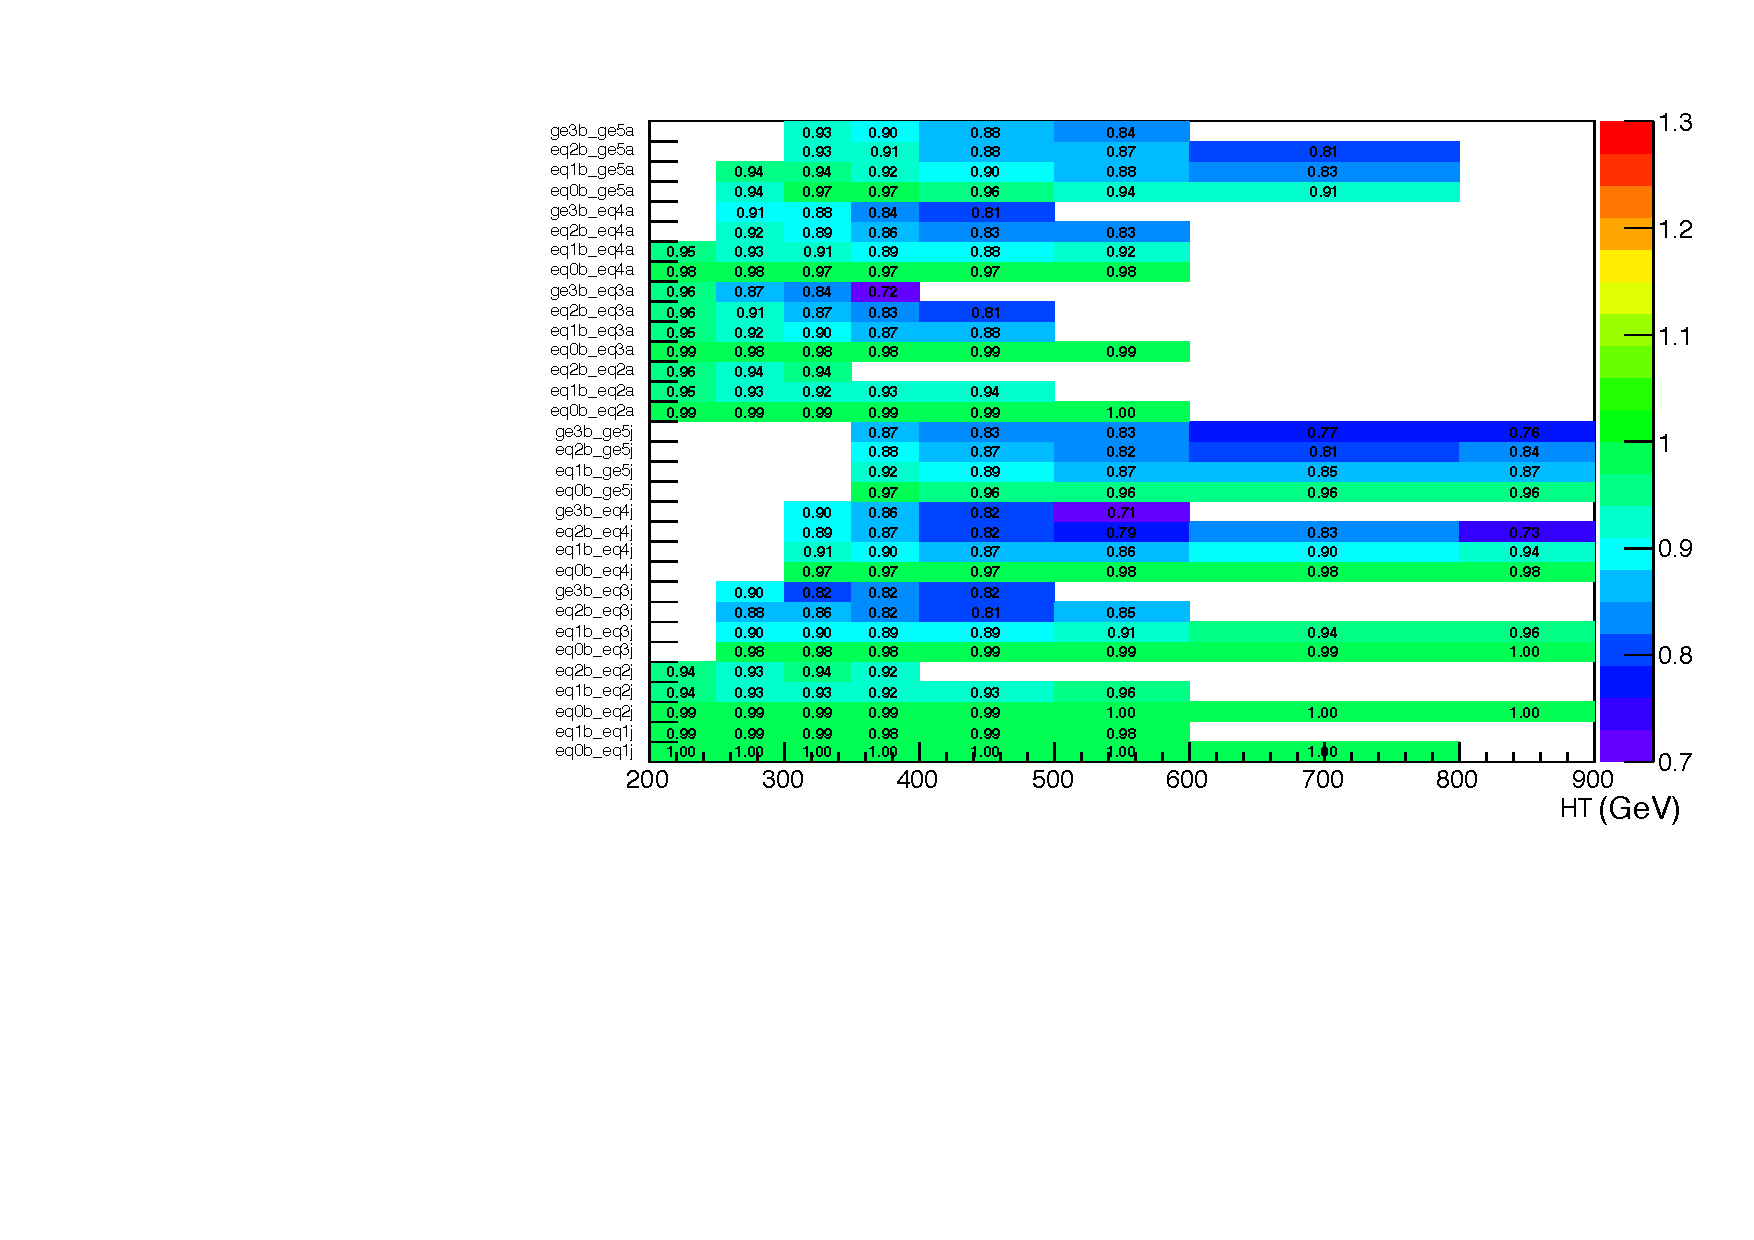
\includegraphics[width=0.45\textwidth]{Figures/backgroundPrediction/mcSystematics12p9fb/Ttw/mu/ratioh_ht_mht_alltopPtWeight_Up.pdf}
  } ~~
  \subfloat[Variation in \mj~to \ttbar/W~transfer factor]{
    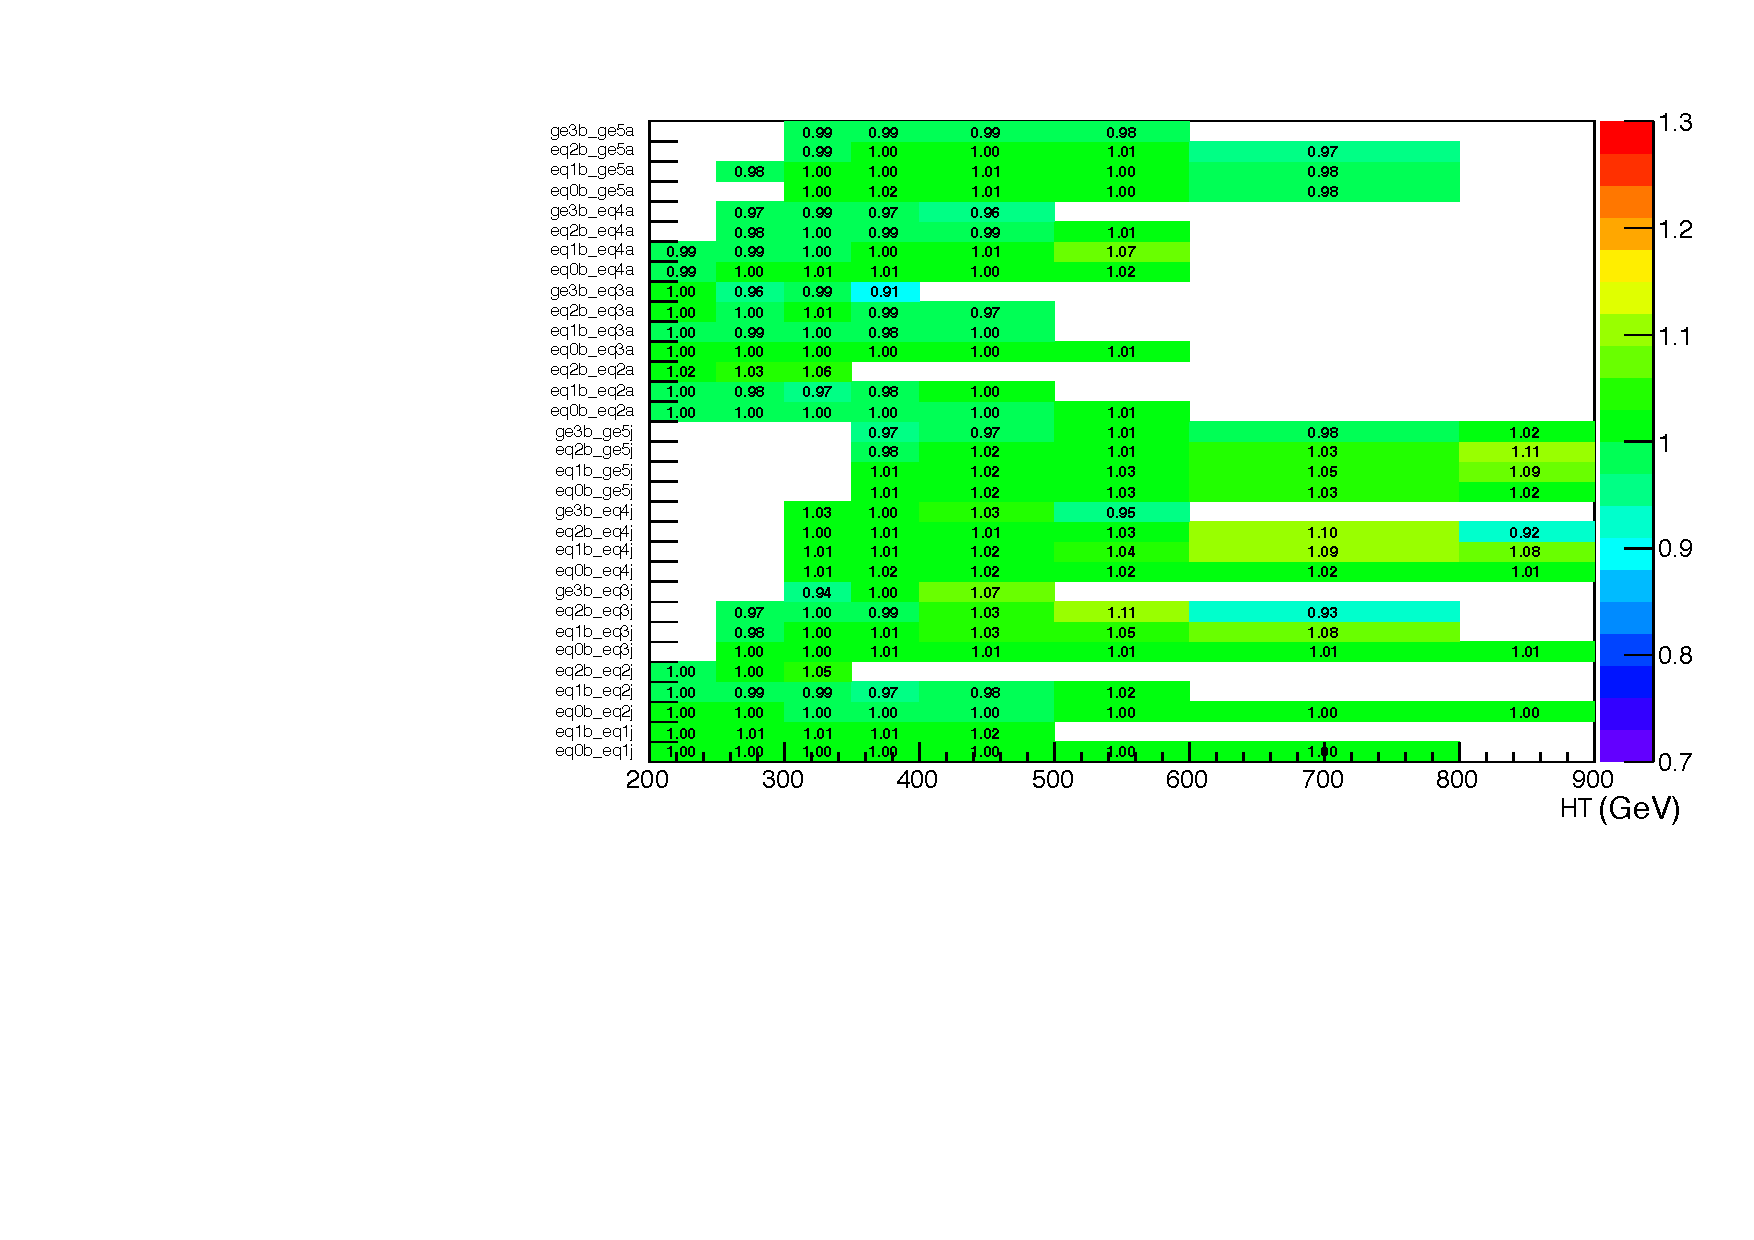
\includegraphics[width=0.45\textwidth]{Figures/backgroundPrediction/mcSystematics12p9fb/Ttw/mu/ratiotfh_ht_mht_alltopPtWeight_Up.pdf}
  }\\
  \caption{\label{fig:tfSimVar} The relative change in the
  \ttbar/W simulation compared to the relative change in the $\mj \rightarrow (\ttbar/W)$ transfer
  factor when varying the top \pt~uncertainty to $+1\sigma$.
  }
\end{figure}

\subsection{QCD background prediction}
\label{sec:qcd-pred}
The prediction of the QCD multijet background is particularly challenging
as it is non-perturbative and has a very large cross section leading to many 
final state topologies that can pass selection. A transfer factor method is used, similar to that used for the electroweak backgrounds. The region used for the prediction is the QCD multijet enriched hadronic control region, 
selected by inverting the signal region selection on \mhtmet. Due to the limited statistical
power of this sample, predictions are made per \njet~and \scalht~category (inclusive in \nb).
Figure~\ref{fig:qcd_plots} shows the QCD multijet events from simulation 
in the hadronic control region and signal region and corresponding transfer factors
between the regions.

The hadronic control region contains a significant electroweak background component, 
as shown in Figure~\ref{fig:ewk_fail}. This component must be accurately predicted
using electroweak enriched control regions (with the \mhtmet~selection inverted) analogously 
to the signal region. The remaining QCD multijet contribution in the control region,
$N_{QCD}^{\rm control}$, then replaces $\nobs^{\rm control}$ in Equation~\ref{equ:pred-method} 
to predict the QCD multijet contribution in the signal region. 

\begin{figure}[!h]
  \centering
  \subfloat[Simulated QCD events in the signal region.\label{fig:qcd_pass}]{
    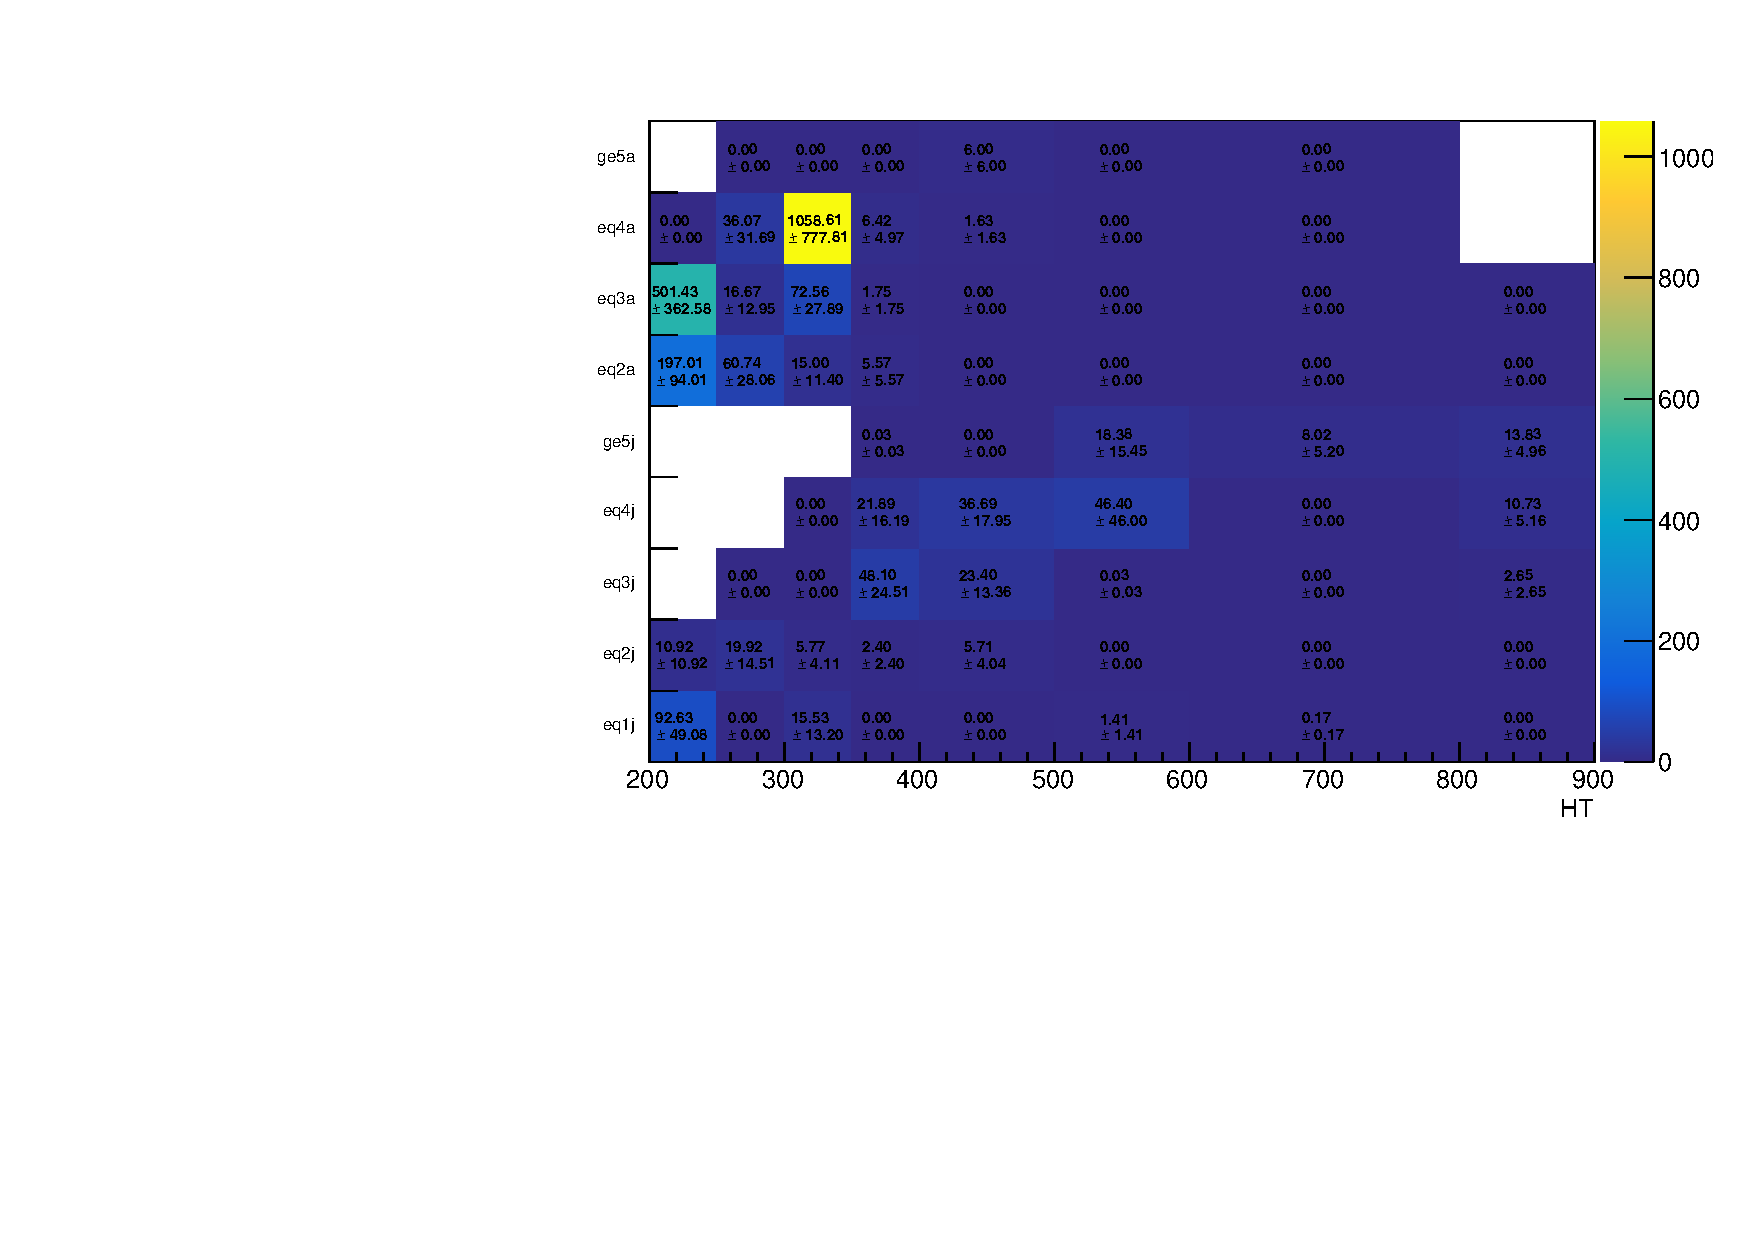
\includegraphics[width=0.45\textwidth]{Figures/qcd/plots/signalQCD_MC}
  } ~
  \subfloat[Simulated QCD events in the \mhtmet~hadronic control region.\label{fig:qcd_fail}]{
    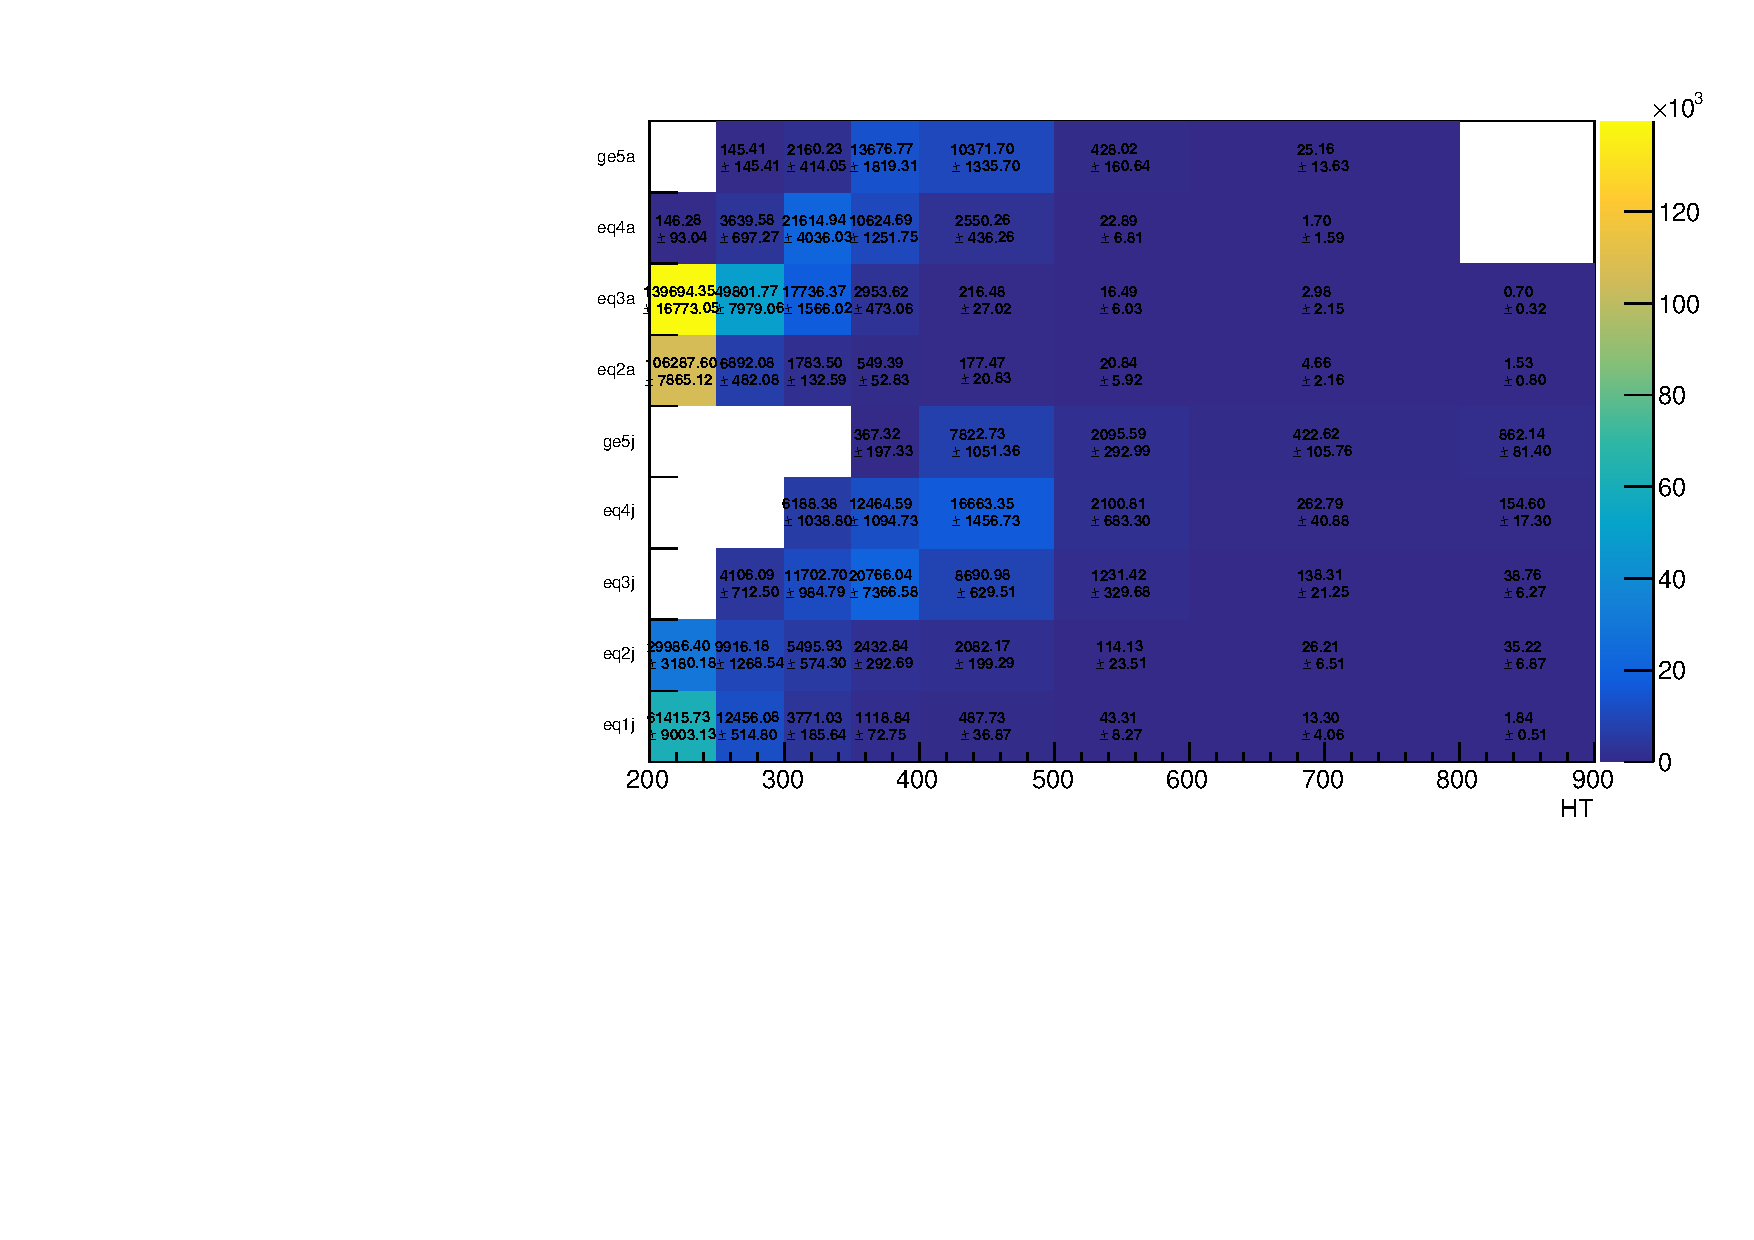
\includegraphics[width=0.45\textwidth]{Figures/qcd/plots/qcdSbQCD_MC}
  } \\
  \subfloat[Transfer factor from simulated QCD events.\label{fig:qcd_ratio}]{
    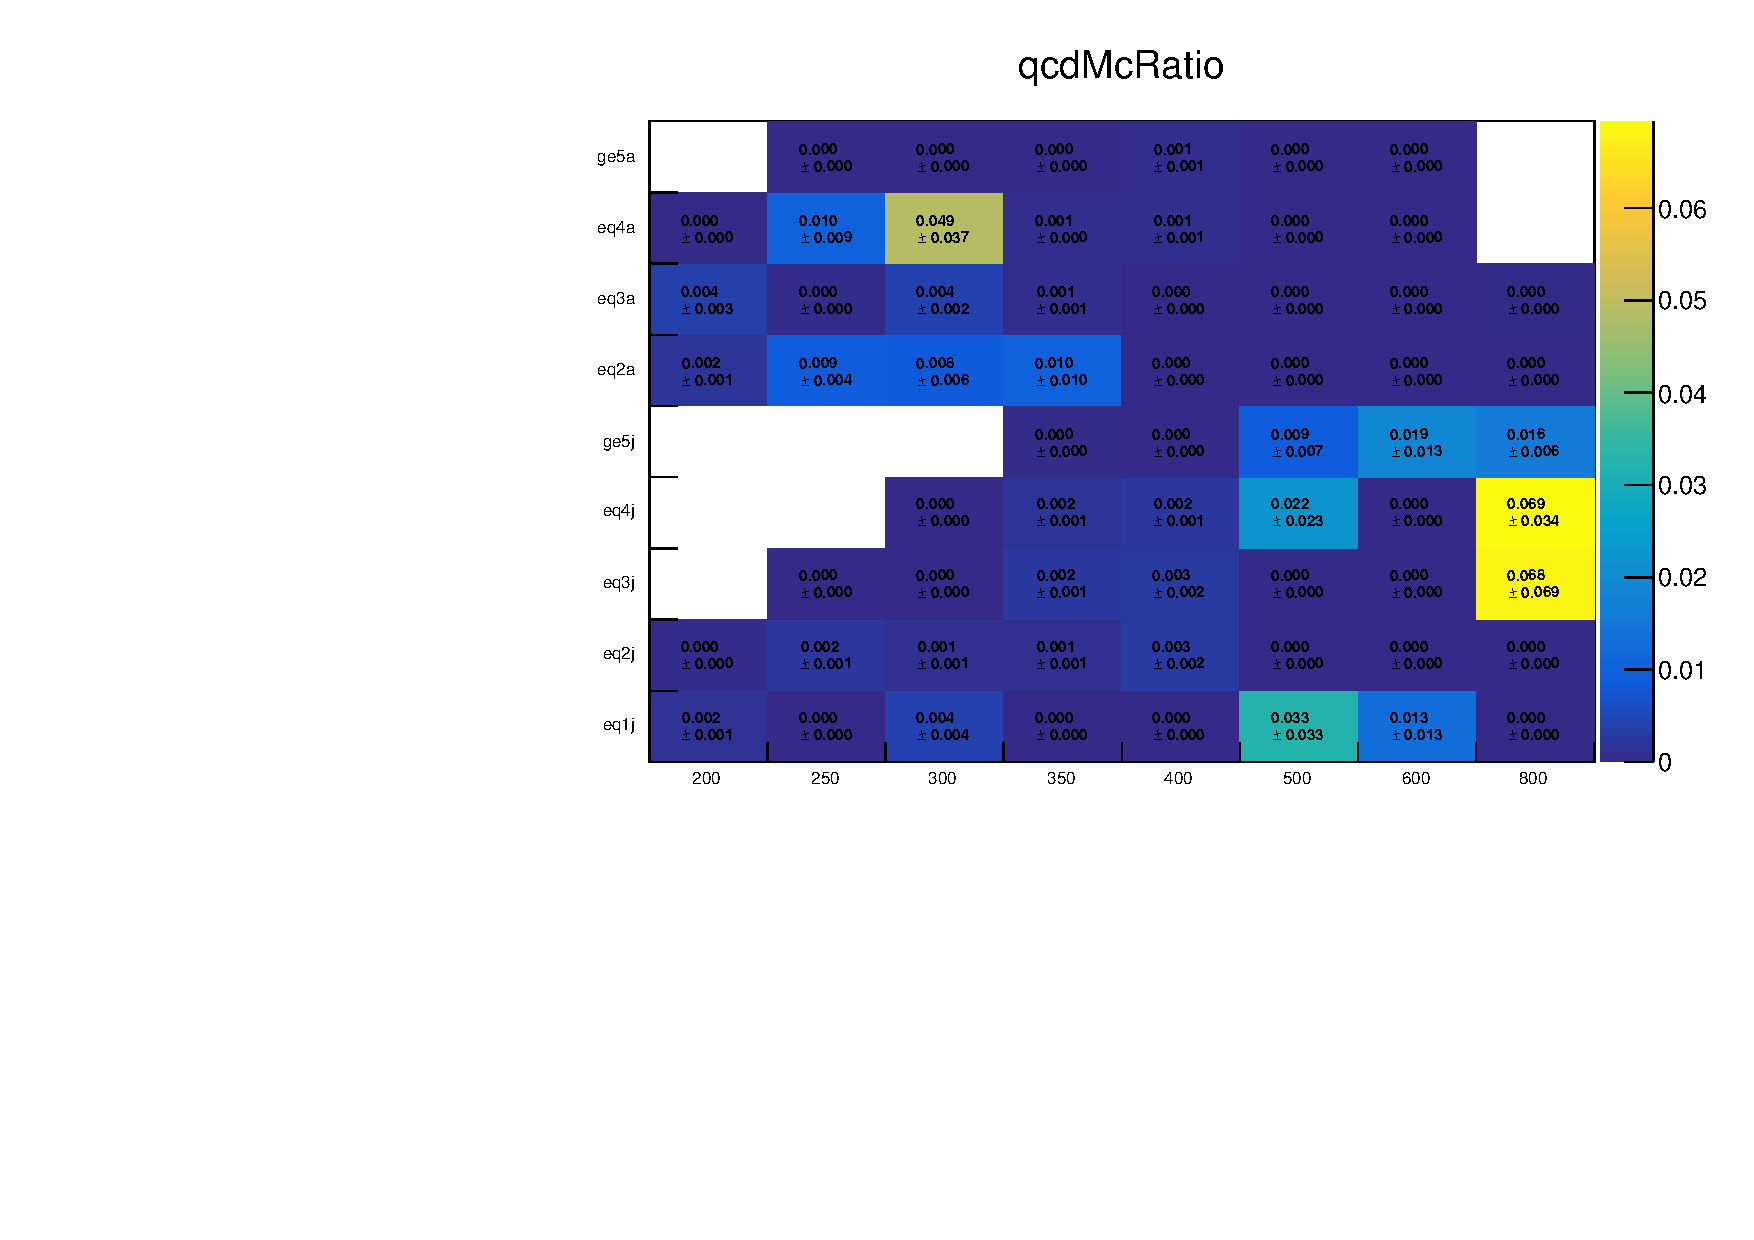
\includegraphics[width=0.45\textwidth]{Figures/qcd/plots/signalQcdDivSbQcd_MC}
  } ~ 
  \subfloat[Simulated electroweak events in \mhtmet~hadronic control region.\label{fig:ewk_fail}]{
    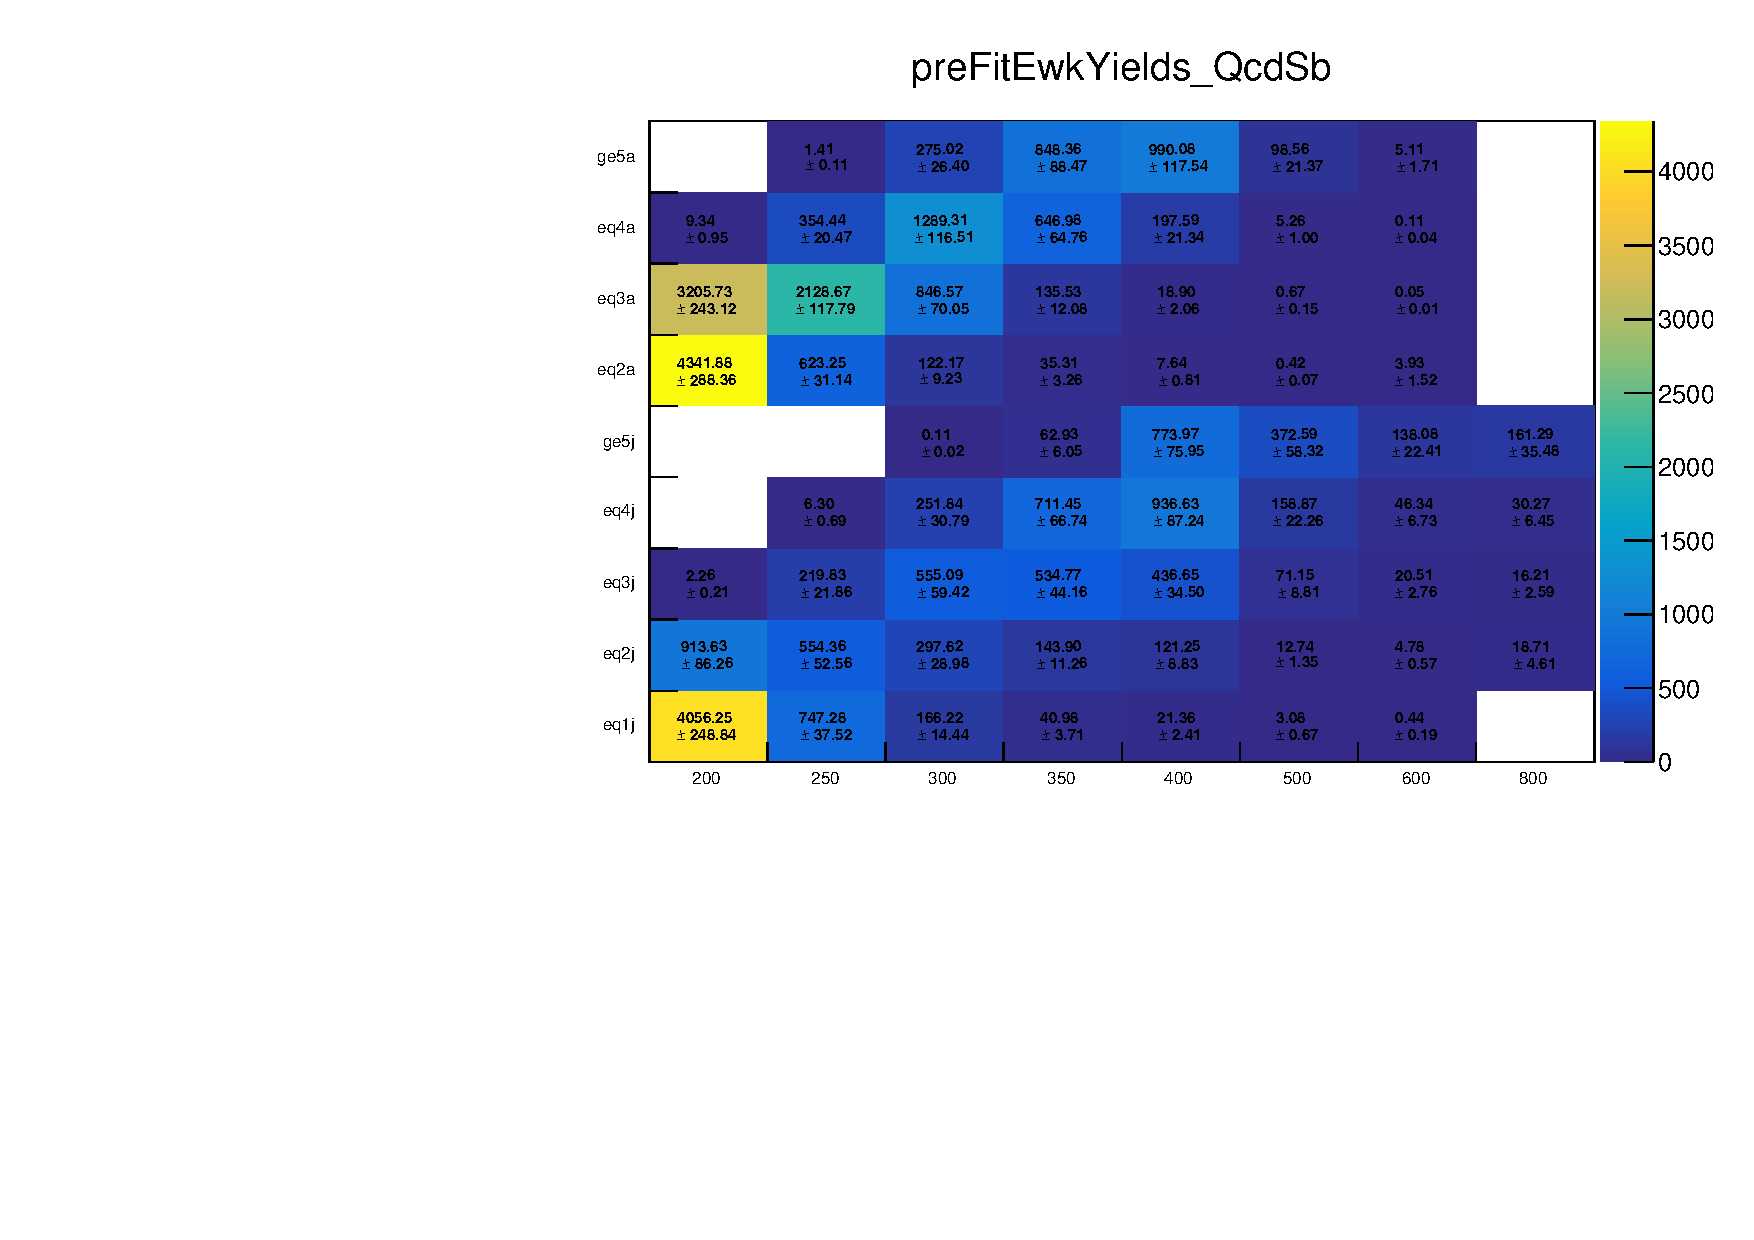
\includegraphics[width=0.45\textwidth]{Figures/qcd/plots/qcdSbEwk_MC}
   %    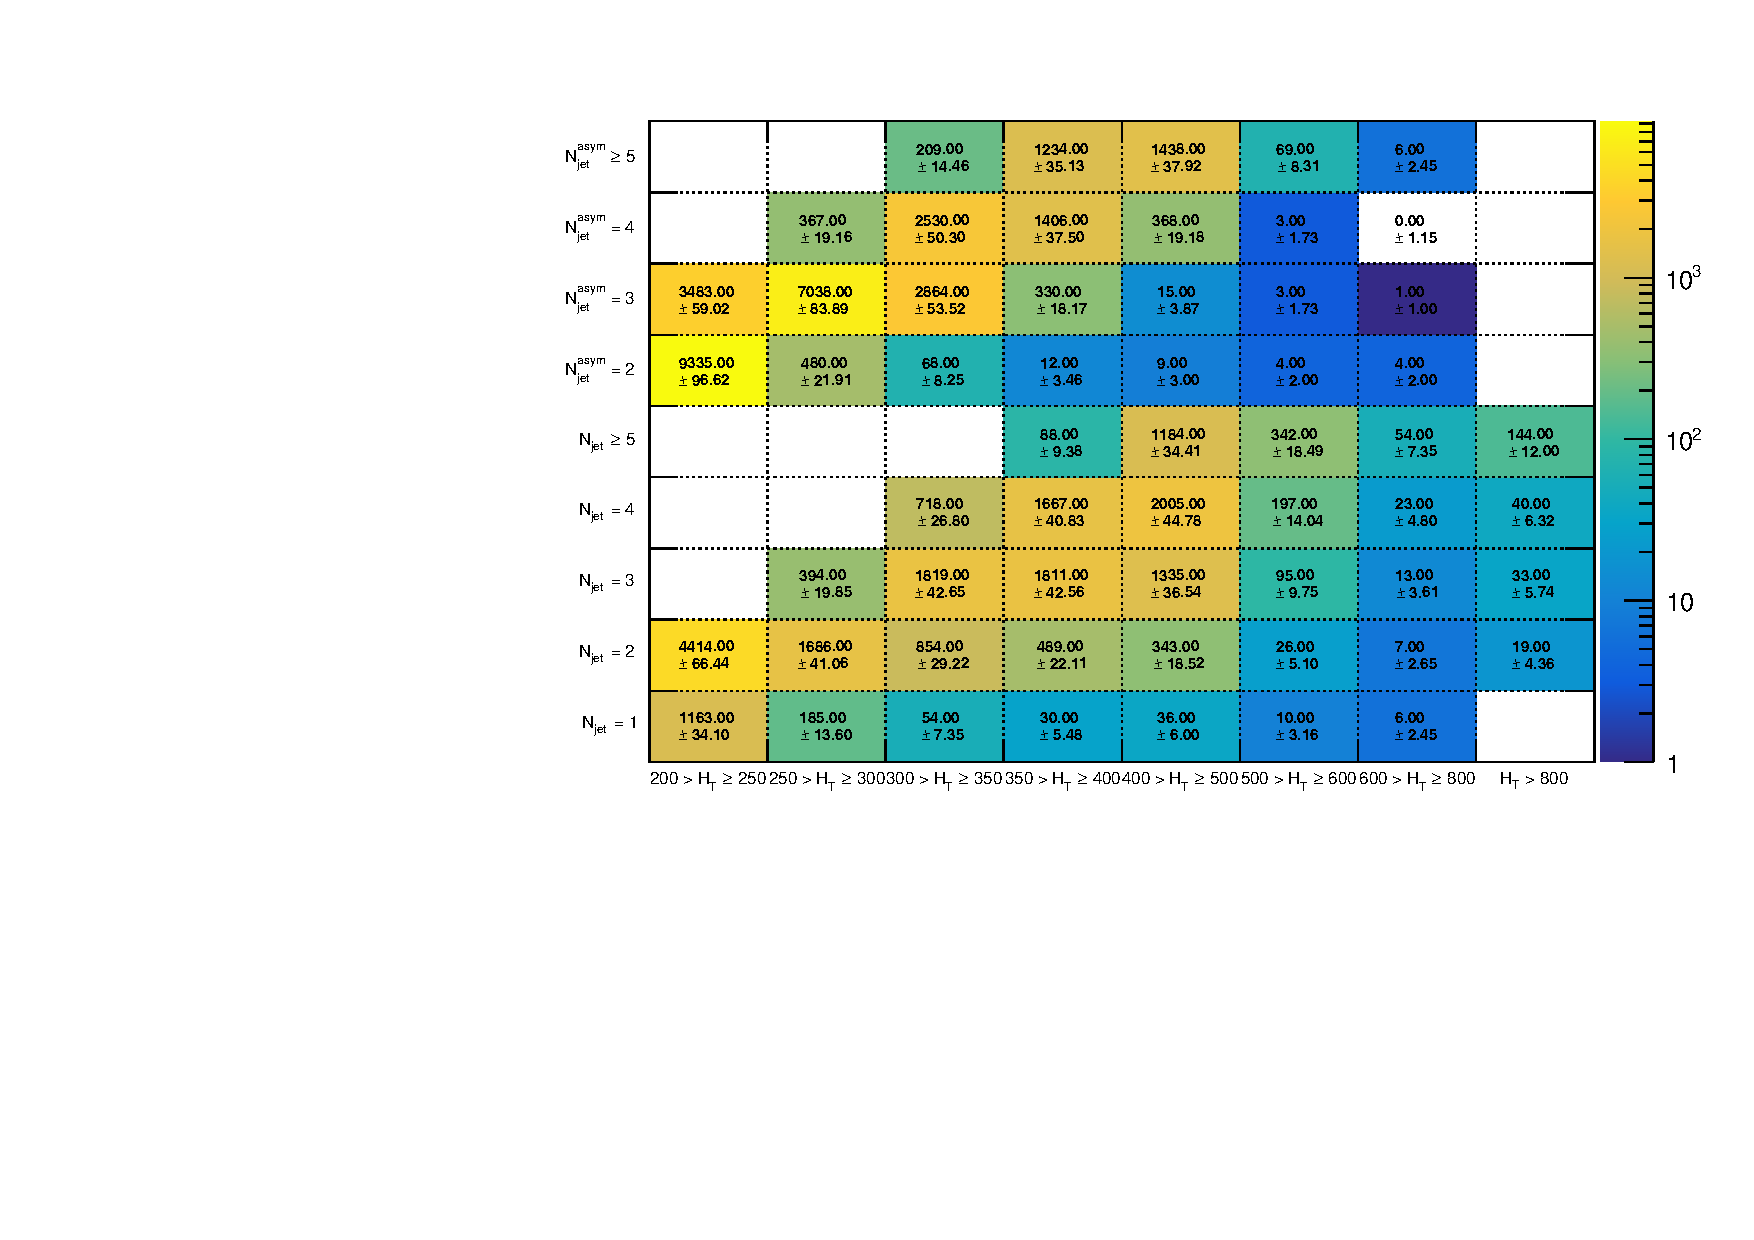
\includegraphics[width=0.45\textwidth]{Figures/qcd/v6/Ewk/SigTrig_FailMoM_NJet_vs_HT_bDPhigt0p5_Log}
  } \\
  \caption{Expected number of QCD multijet events determined from
    simulation, binned according to \njet~and \scalht, that (a) satisfy
    and (b) fail the requirement $\mhtmet < 1.25$. Also shown in (c)
    is the transfer factor for QCD multijets from hadronic control to signal region, 
    again determined from simulation. Finally, (d) shows the expected number of electroweak 
    background events (V+jets and \ttbar, plus other residual non-multijet backgrounds)
    that fail the $\mhtmet < 1.25$ requirement, again determined from
    simulation and binned according to \njet~and \scalht.}
  \label{fig:qcd_plots}
\end{figure}

To determine the electroweak predictions in the hadronic control region transfer factors 
from the \mhtmet~electroweak control regions are constructed and a simultaneous
fit is carried out, similar to that described in Section~\ref{sec:likelihood} for the signal region. 
This fit includes all systematic variations discussed in Section~\ref{sec:syst-uncs}, 
derived with the \mhtmet~selection inverted. An unconstrained contribution in the fit, 
uncorrelated in each \njet~and \scalht~category, is included to measure the difference between 
the electroweak prediction and the observation. This is taken as $N_{QCD}^{\rm control}$ in each bin and
the values per \njet~and \scalht~category, including systematic and statistical uncertainty,
are shown in Figure~\ref{fig:data_corr}. 

The signal region prediction is then made by multiplying the QCD multijet component in the hadronic 
control region by the transfer factors shown in Figure~\ref{fig:qcd_ratio}. The results of this prediction
are shown in Figure~\ref{fig:qcd_pred}, with the ratio between the multijet and non-multijet background
predictions shown in Figure~\ref{fig:qcd_ewk_ratio}. The multijet component is typically $\le 5\%$. 

\begin{figure}[!h]
  \centering
  % \subfloat[Binned data counts in \mhtmet sideband.\label{fig:data_fail}]{
  %   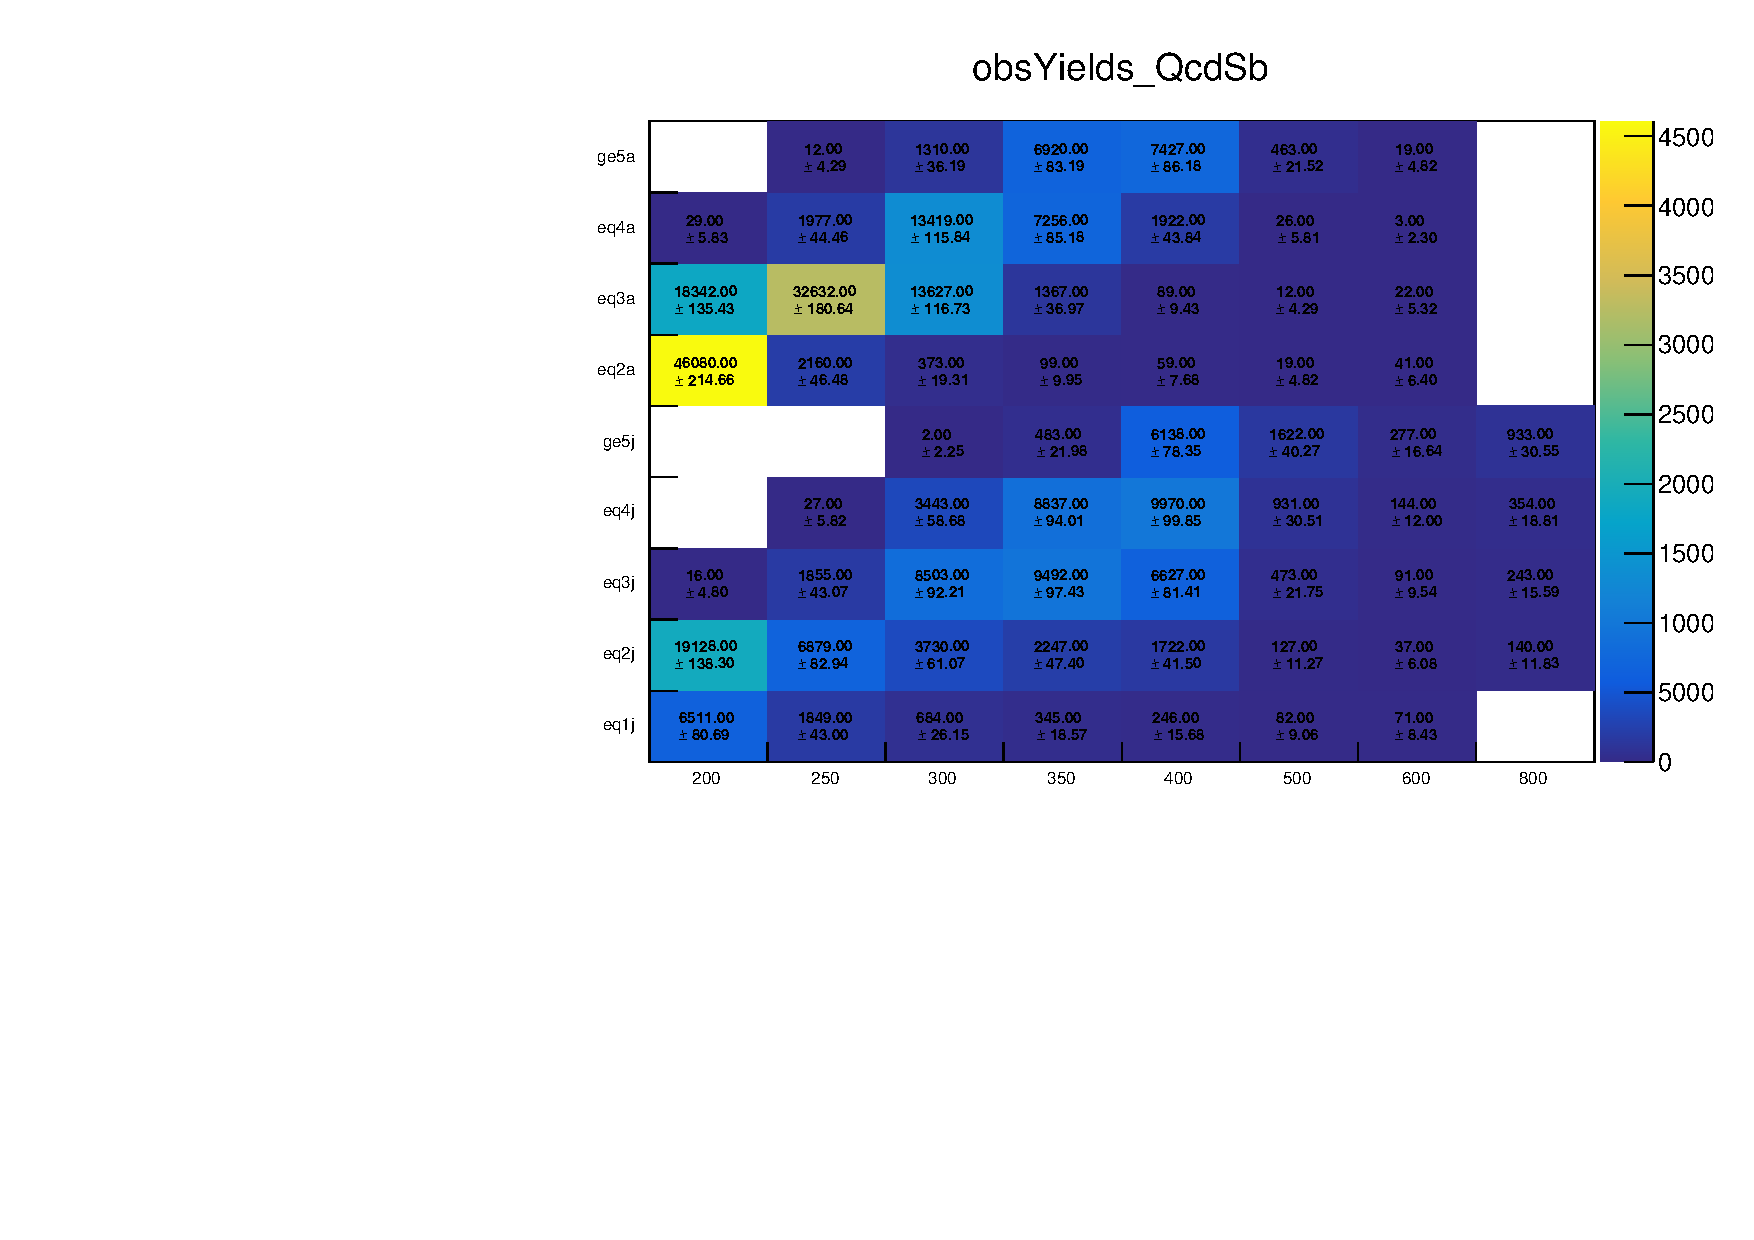
\includegraphics[width=0.45\textwidth]{Figures/qcd/plots/obsYields_QcdSb}
  % } 
  \subfloat[Predicted QCD counts in the \mhtmet hadronic control region.\label{fig:data_corr}]{
    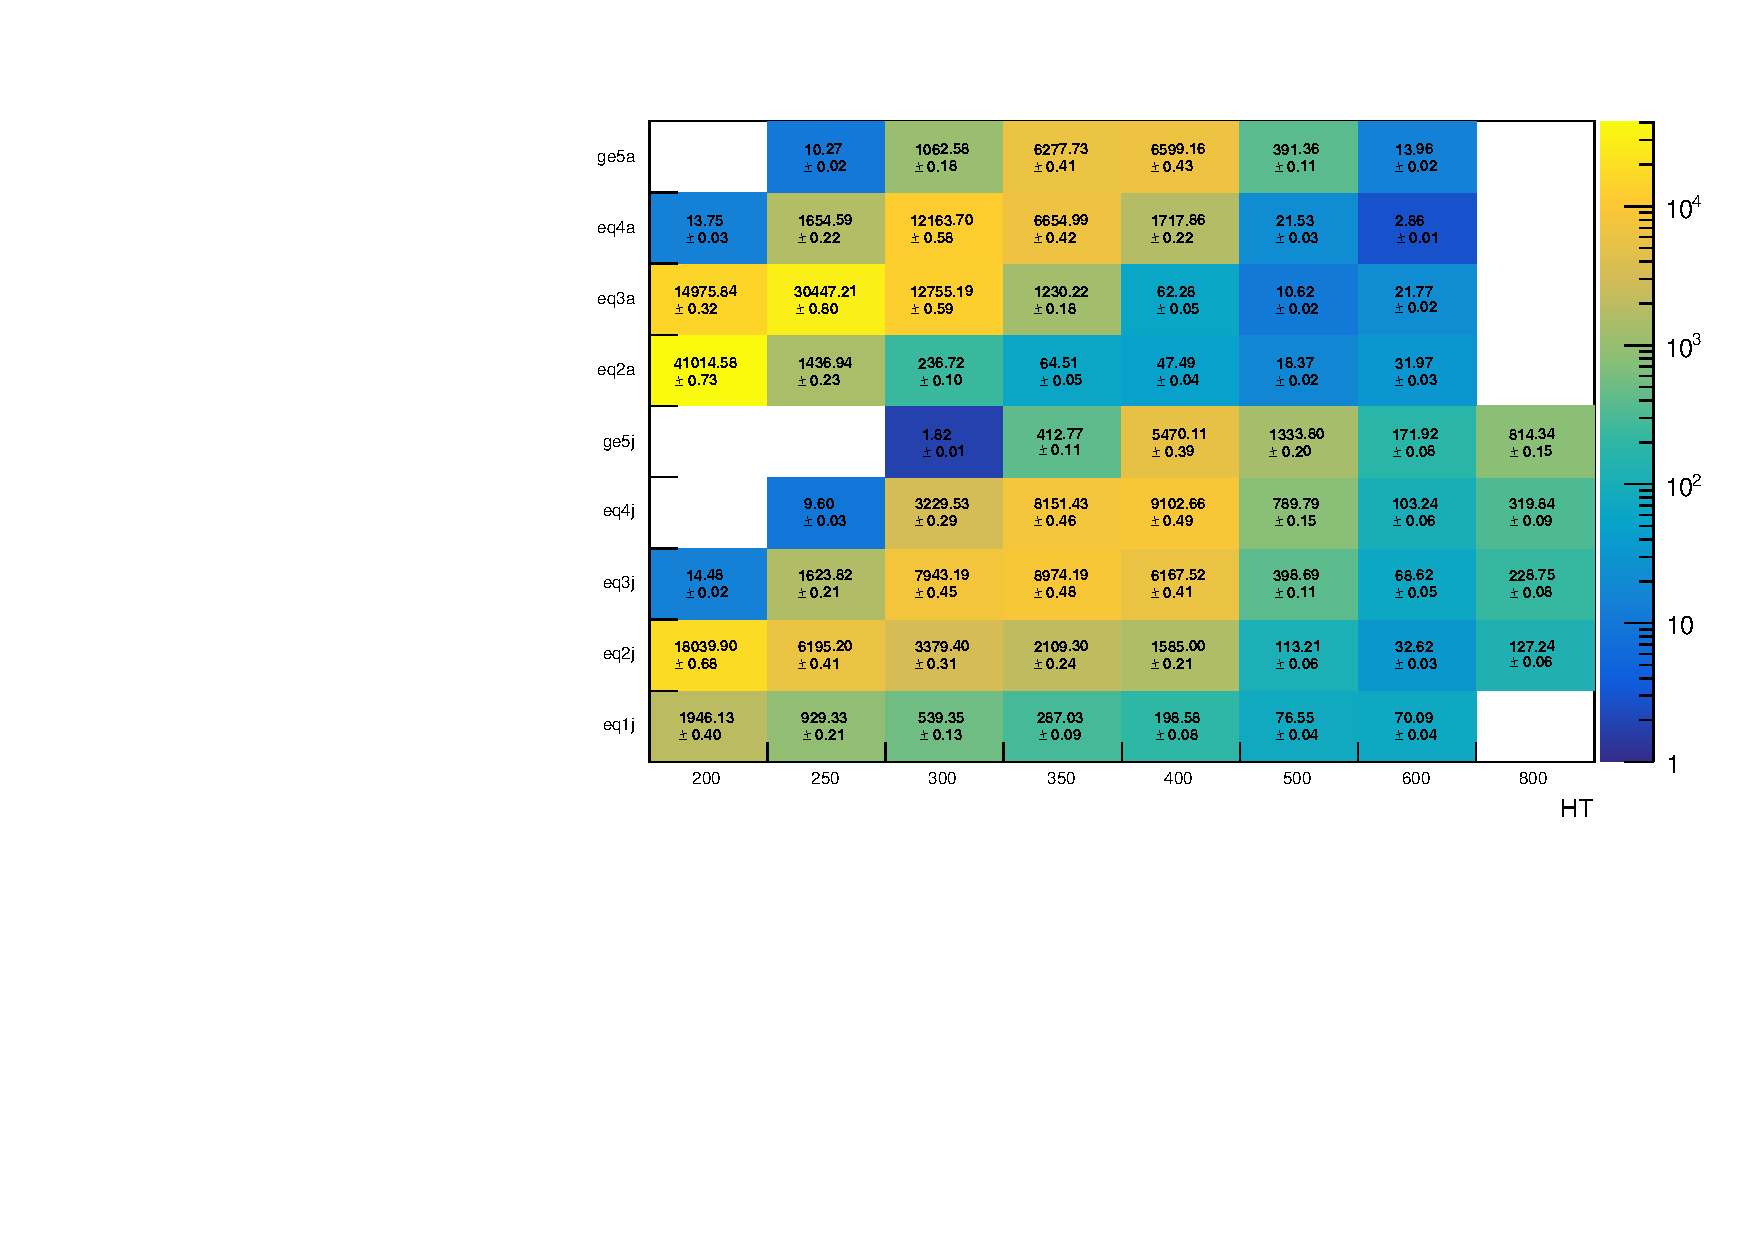
\includegraphics[width=0.45\textwidth]{Figures/qcd/plots/postFitQcdYields_QcdSb}
  } ~
  \subfloat[QCD multijet predictions in the signal region.\label{fig:qcd_pred}]{
    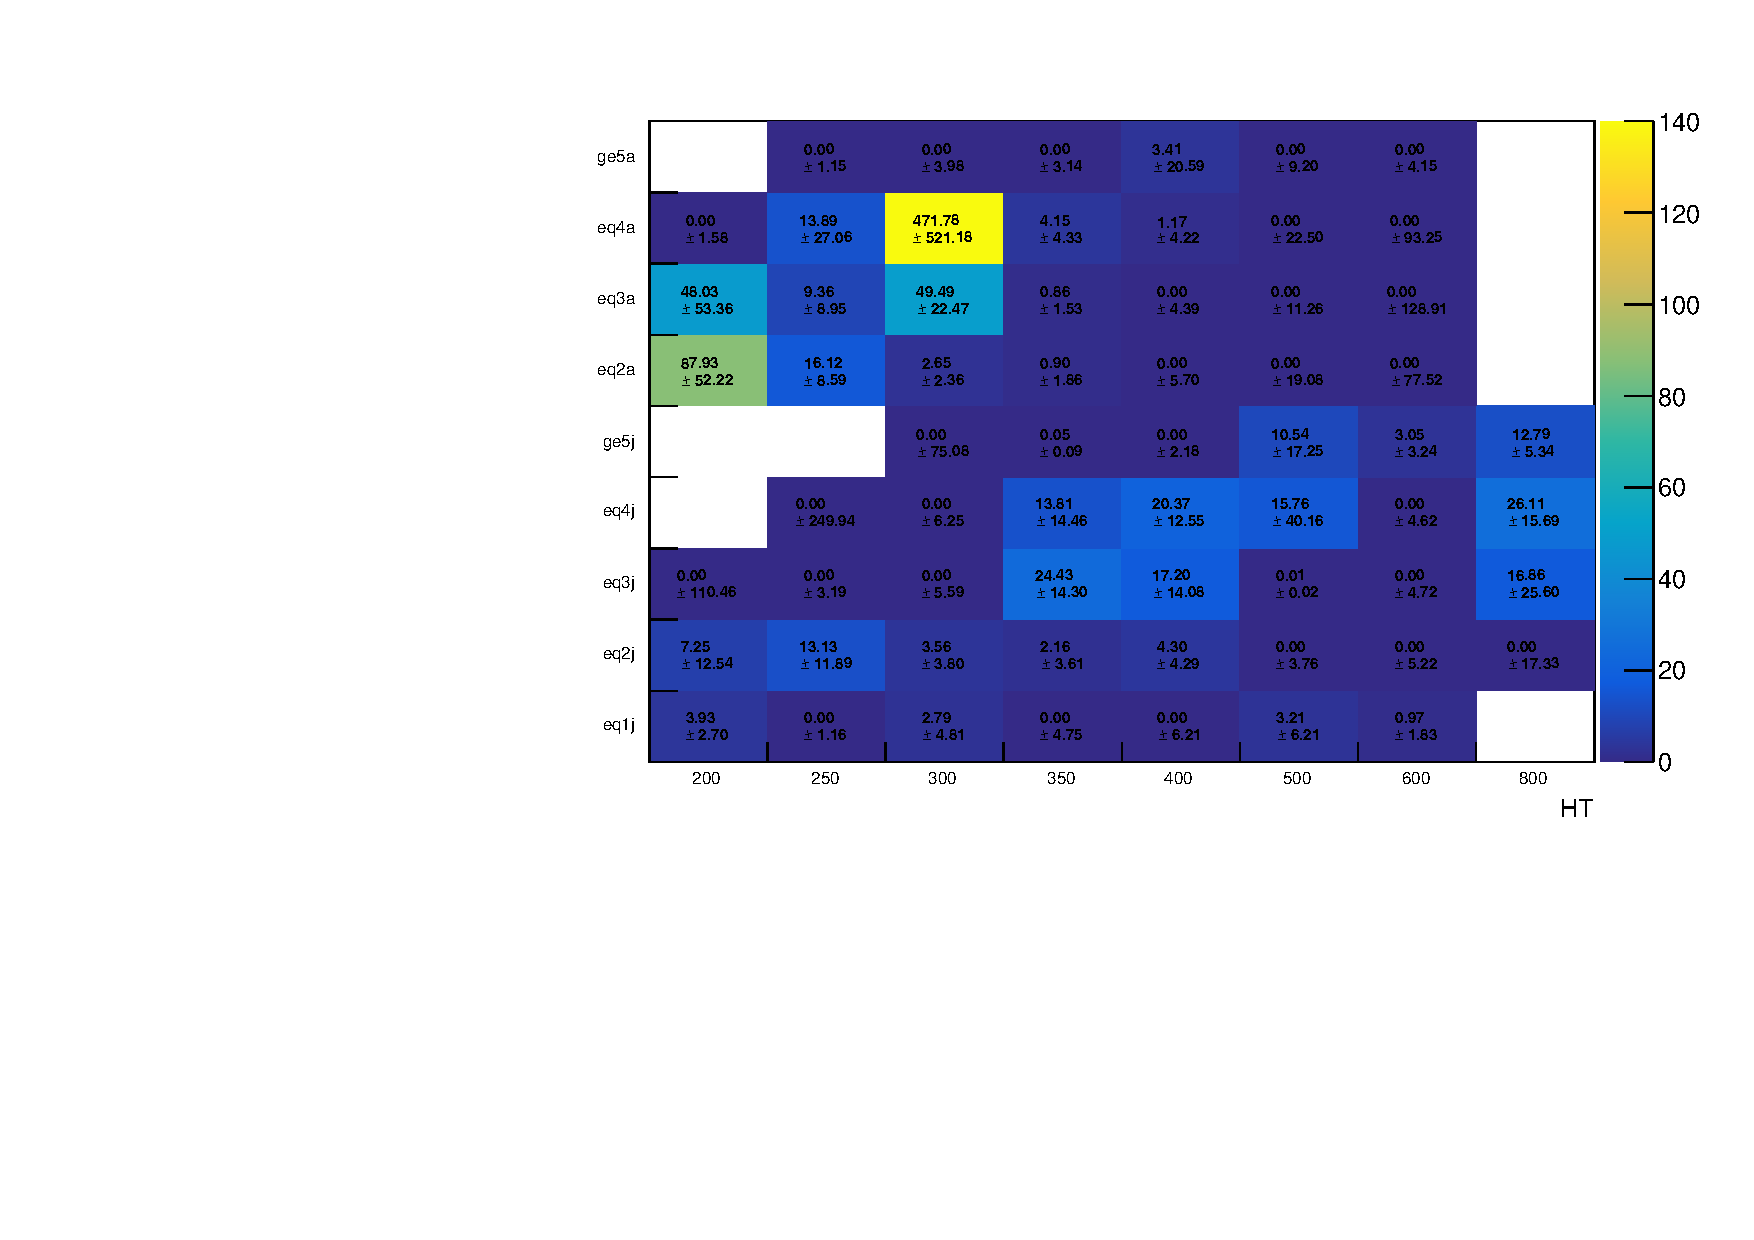
\includegraphics[width=0.45\textwidth]{Figures/qcd/plots/predictedQcdYields_Signal}
  } \\
  \subfloat[Ratio of predicted multijet and non-multijet yields.\label{fig:qcd_ewk_ratio}]{
    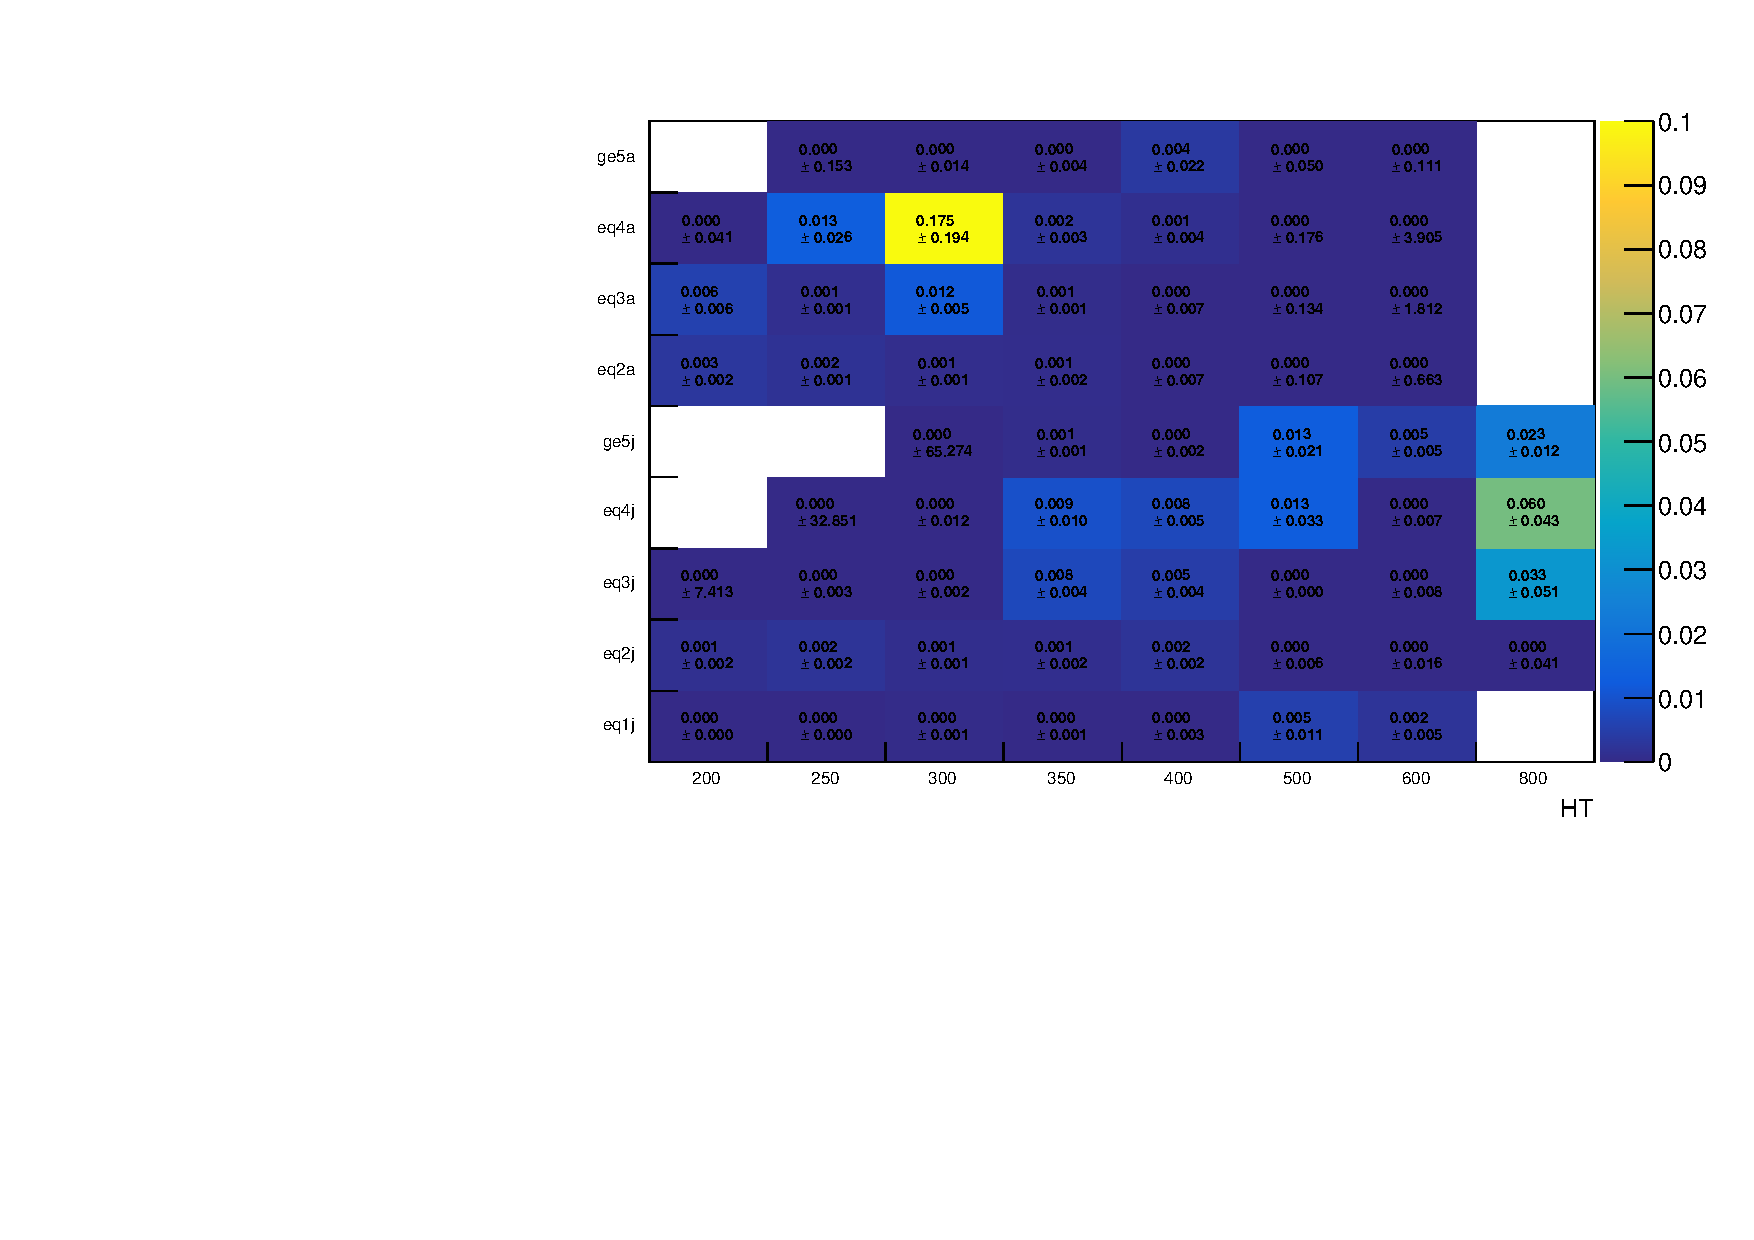
\includegraphics[width=0.45\textwidth]{Figures/qcd/plots/predictedQcdDivEwk_Signal}
  } \\
  \caption{
    The QCD yields taken from the simultaneous fit binned according to \njet~and \scalht~are shown in (a).
    Shown in (b) is the result of multiplying the observed multijet events predicted
    in (a) by the translation factor from the sideband to the signal
    region determined with simulation (shown in
    Figure~\ref{fig:qcd_plots}). This gives a data-driven expectation of
    the quantity of multijet background events in the signal region. 
    Finally, (c), shows the ratio of expected
    multijet background events in the signal region divided by
    non-multijet backgrounds. The multijet background is therefore
    shown to be at the percent level.}
  \label{fig:qcd_plots2}
\end{figure}

The distribution of the QCD multijet contribution in \nb ~and \mht~in each \scalht~and \njet~category
is predicted using the distribution of the electroweak background with the normalisation
derived as described above. This approximation is necessary due to the very low QCD multijet
event yields for high \nb ~and \mht. As the multijet background is typically $\le 1\%$, 
deviations from the electroweak shape in these variables have a small effect on the background prediction.

The multijet contribution in the electroweak control regions is small, typically $\le 1\%$, and is 
therefore taken from simulation.

\subsubsection{Validation of the multijet prediction}

The QCD multijet prediction relies on an extrapolation in the \mhtmet~requirement.
Significant mismodelling of this variable can bias the QCD prediction and therefore a validation
of this extrapolation is carried out using an additional hadronic control 
region which is defined by inverting the $\bdphi > 0.5$ requirement. The ratio of events passing and failing 
the requirement $\mhtmet < 1.25$ is made in data and simulation, $\mathcal{R}^{data}$ and $\mathcal{R}$ respectively,
in categories of \njet~and \scalht. The ratio of $\mathcal{R}^{data}$ to $\mathcal{R}$ is shown in
Figure~\ref{fig:RR_qcd} (excluding bins with insufficient statistics). 
Given the level of agreement, a fully correlated systematic uncertainty of $100\%$ is included on
the QCD contamination. This is included in addition to the systematic uncertainties shown in 
Figure~\ref{fig:qcd_pred}, taken as uncorrelated in each category.

\begin{figure}[h!]
  \begin{center}        
    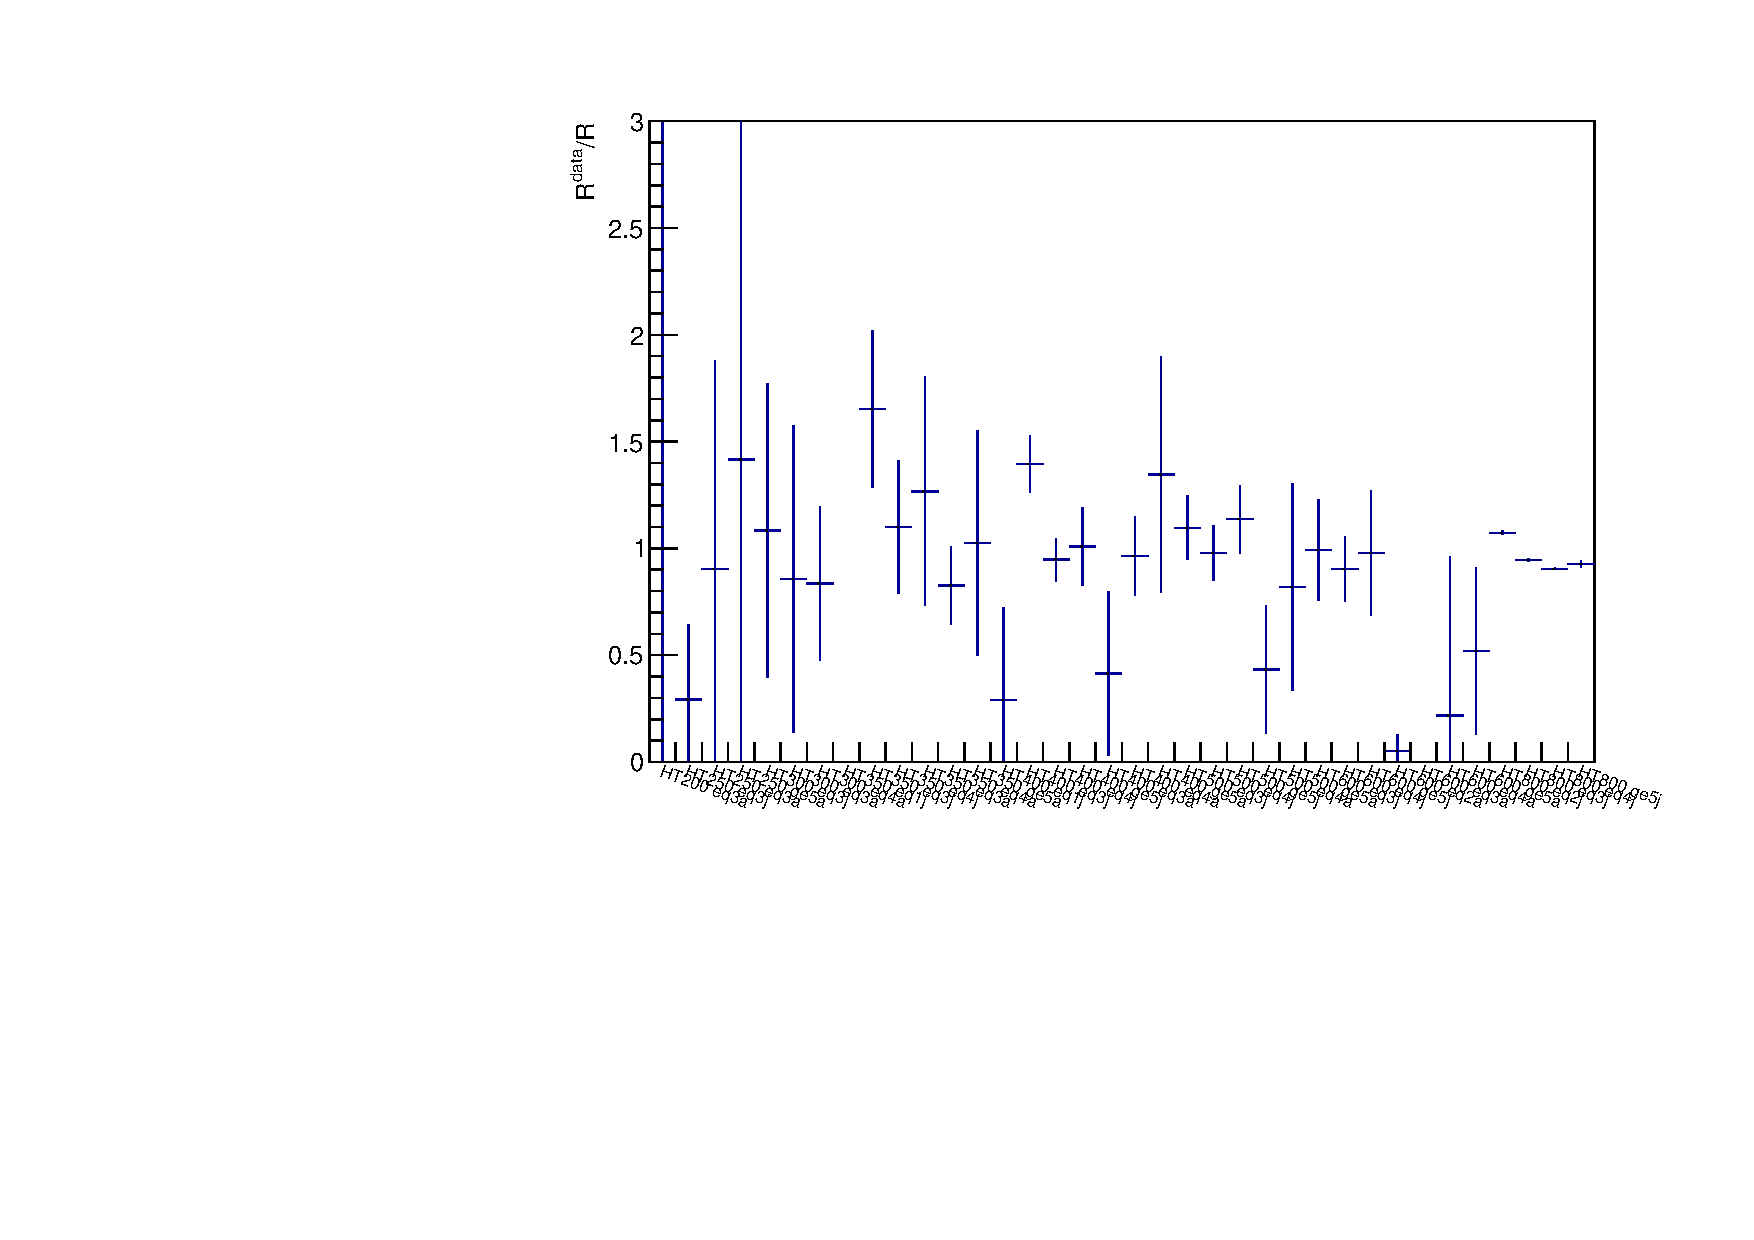
\includegraphics[width=0.6\textwidth]{figures/qcd/plots/doubleQcdSbSrRatio1D}
    \caption{ Ratio of the measurement of \rmhtmet, the pass/fail ratio for the \mhtmet~selection, from data and Monte Carlo in the $\bdphi < 0.5$ sideband in (\scalht, \njet) bins.  
    }
    \label{fig:RR_qcd}
  \end{center} 
\end{figure}

\section{Systematic uncertainties in the transfer factors}
\label{sec:syst-uncs}
This section describes the determination of systematic uncertainties 
in the transfer factors through both variations of simulation
and using the data-driven `closure tests'. 

\subsection{Variation method}
\label{sec:syst-uncs-var}
The corrections applied to the simulated samples are summarised in Section~\ref{sec:corr-sim}. For each 
simulated event the correction may apply to the weight carried by that events (such as b tag efficiency
or pile-up reweighting) or to the property of objects in the event (such as the jet energy scale). 
These corrections carry uncertainties that may affect the predictions of the \alphat~analysis.
To determine the effect of each such source of systematic uncertainty, the correction is varied to $\pm$ 1 $\sigma$ from its central value and the prediction from simulation is re-evaluated. The inclusion of the systematic uncertainty 
in these predictions, in particular how the modifier term morphs between alternative `templates'  
for $\pm$ 1 $\sigma$ variations, is described in Section~\ref{sec:likelihood}. In this section the systematic variations
of the transfer factor for each effect is discussed. The effect of these systematics on 
the \mht~shape is discussed in Section~\ref{sec:syst-on-shape}.

\subsubsection{Pileup reweighting}

The uncertainty on the inelastic p-p cross section of $\pm5\%$ is propagated by deriving the pile-up
weights for the cross section at the $\pm1\%$ sigma values. These weights are used to derive
alternative predictions for each variation. Typically, the uncertainty 
introduced by pile-up reweighting is small, up to $\sim2\%$ depending on the category.

\subsubsection{Jet energy scale}
The energies of jets used in the analysis are corrected as a function of their \pt~and
$\eta$ via the procedure described in Section~\ref{sec:jec}. The uncertainty on
this correction is propagated through the analysis. As the \scalht~and jet multiplicity binning is 
mirrored in signal and control regions, the variation in the transfer factors is small.
To avoid statistical fluctuations, the variation is averaged across~\nb.
The systematic variations are typically in the range of $1$ to $5\%$ depending on the category.

\subsubsection{B-tagging efficiency}

Scale factors are applied to simulation to correct for differences in the 
b tagging efficiencies and misidentifications between simulation and data. 
Since no extrapolation is performed in the background prediction across different 
\nb~ multiplicities, the analysis is expected to be robust against variations in the 
b tagging efficiency. The scale factors associated with b and c jets are varied together 
(since their measurements are correlated), while those associated with light jets are varied separately.
The systematic variations are typically in the range of $1$ to $3\%$ depending on the category.

\subsubsection{Lepton trigger/identification/isolation efficiency}

Leptons out of \pt~and $\eta$ acceptance, or within detector
acceptance but not identified properly by lepton identification or isolation
requirements contribute to the lost lepton background. The variation 
in the lost lepton background is measured using a simulated sample with no lepton veto.
Using this sample, the variation in probability for reconstructing a lepton in the signal region,
and the variation for reconstructing a muon for the \mj~control region is determined with 
appropriate correlation. The systematic uncertainties from trigger, identification and 
isolation efficiencies on the muon and electron scale factors are varied separately. 
An additional uncertainty is considered on the~\mj~control region for the muon tracking
scale factor. The systematic variations are typically in the range of $1$ to $3\%$ depending on the category.

\subsubsection{Photon trigger uncertainty}
The photon trigger correction is derived for the \gj~control region. The systematic uncertainty is
taken as the size of the measured inefficiency. The systematic variation in the \gj~transfer factors 
is typically under $\sim3\%$.

\subsubsection{Signal trigger uncertainty}

The systematic on the signal trigger efficiency is taken as the difference in the 
efficiency measured using muon and electron reference triggers. 
This uncertainty affects only the signal region predictions
and not the control region predictions. The systematic variation in the transfer factors is 
typically in the range $1$ to $6\%$.

\subsubsection{Top \pt~reweighting}
The uncertainty in the top \pt~reweighting is taken as the size of the reweighting
applied to each event. The systematic variation in the transfer factors is typically in the range
$1$ to $7\%$.

\subsection{Closure test method}
\label{sec:closure-tests}
The variations described above cover systematic uncertainties that can be easily assessed 
from simulation. In addition, the data in the control samples are used to
further probe sources of bias in the transfer factors due to limitations in the simulation.
The events of one control sample, B, are predicted using events from another control sample, A,
using a transfer factor from the ratio in simulation, 

\begin{equation}
\label{equ:abPred}
N^{B}_{\text{pred}} = N^{B}_{\text{sim}}/N^{A}_{\text{sim}} \times N^{A}_{\text{data}} = TF_{\text{AB}} \times N^{A}_{\text{data}}.
\end{equation}

The agreement between the observation in sample B and the prediction from sample A is measured by the ratio

\begin{equation}
R_{\text{AB}} = \frac{N^{A}_{\text{data}}-N^{B}_{\text{pred}}}{N^{B}_{\text{pred}}}.
\end{equation}


The closure between the samples is defined as the significance of the deviation of this ratio from zero 
considering statistical uncertainties in both observation and simulation in samples A and B.
The tests are performed separately per \njet~and \scalht~category to investigate the level of closure. 
The uncertainties are derived per \scalht~bin by merging the \njet~categories into 
the symmetric and asymmetric (including monojet) topologies. For each such category, the systematic
uncertainty is defined by the value of $R_{\text{AB}}$ added in quadrature to its statistical uncertainty.
For tests involving the \mmj~sample, which has lower statistical power, pairs of \scalht~bins 
are merged for the closure tests. The closure tests are carried out between control regions or a subset
of the control regions and therefore probe bias in events with a similar composition to those in the signal regions.

The systematics derived using these tests are applied to the transfer factors. They are considered
as uncorrelated per \scalht~and jet topology (monojet and asymmetric topologies are correlated) and correlated in other categorisations. The tests carried 
out and systematic biases probed are discussed below.

\subsubsection{Extrapolation in \alphat~and \bdphi}

The extrapolation in \alphat~and \bdphi~from the \mj~and \mmj~control regions 
and in \bdphi~for the \gj~control region to the signal region may introduce bias
 due to modelling differences in data and simulation. To test the \alphat~(\bdphi) modelling the \mj~sample is divided 
into events with an \alphat~(\bdphi) requirement and with this requirement inverted.
The \alphat requirement is decided by the signal \scalht~bin 
and the \bdphi requirement is 0.5. The systematic is derived from the \alphat~closure tests for
bins with $\scalht < 800\,\GeV$ and from the \bdphi~tests for $\scalht > 800\,\GeV$.

The results of these tests are shown in Figure~\ref{fig:closureAlphaT} as a function of \scalht~and \njet. 
The grey band is the systematic uncertainty propagated through the analysis. 
The systematic derived from these tests is
in the range $4$ to $32\%$.

\begin{figure}[h!]
  \begin{center}
    \subfloat[]{\includegraphics[width=0.45\textwidth]{Figures/backgroundPrediction/closureTests/alphaT_sym__noFit.pdf}}
    ~~
    \subfloat[]{\includegraphics[width=0.45\textwidth]{Figures/backgroundPrediction/closureTests/alphaT_asym__noFit.pdf}}\\
    \subfloat[]{\includegraphics[width=0.45\textwidth]{Figures/backgroundPrediction/closureTests/bDPhi_sym__noFit.pdf}}
    ~~
    \subfloat[]{\includegraphics[width=0.45\textwidth]{Figures/backgroundPrediction/closureTests/bDPhi_asym__noFit.pdf}} 

    \caption{Tests in data probing the \alphat~(top row) and \bdphi~(bottom row) extrapolation for each
      \njet~category (open symbols) overlaid on top of the systematic
      uncertainty estimates used for each of the seven \scalht~bins (shaded bands). 
      The symmetric (asymmetric) jet topologies are shown in the left (right) plot. 
    }
    \label{fig:closureAlphaT}
  \end{center} 
\end{figure}
\subsubsection{Modelling of the W acceptance due to polarisation effects}

The high \pt W bosons produced in p-p collisions are predominantly left-handed~\cite{lhW}. 
There is no right-handed neutrino and therefore the $W^{+}$ bosons 
preferentially decay to the (left-handed) neutrino along 
its direction of motion while the lepton points backwards. 
The $W^{-}$ bosons behave oppositely, decaying
to the lepton along its direction of motion. 

\wj events typically pass signal region selection due to
the presence of a boosted neutrino while such events typically
pass \mj~control region selection due to the presence of a boosted lepton.
There is therefore a preponderance of $W^{+}$ over $W^{-}$ in the 
signal region compared to the \mj~control region. This may introduce bias
in the prediction and a data-driven test is carried out by splitting the \mj~sample into events 
with either a $\mu^{+}$ or $\mu^{-}$.

The results are shown in Figure~\ref{fig:closureMuPToMuM} as a function of \scalht~and \njet. 
The grey band is the systematic uncertainty propagated through the analysis.
The systematic derived from these tests is in the range $3$ to $12\%$.



\begin{figure}[h!]
  \begin{center}
    \subfloat[]{\includegraphics[width=0.45\textwidth]{Figures/backgroundPrediction/closureTests/muplus_muminus_sym__noFit.pdf}}
    ~~
    \subfloat[]{\includegraphics[width=0.45\textwidth]{Figures/backgroundPrediction/closureTests/muplus_muminus_asym__noFit.pdf}} 
    \caption{Data-driven tests probing the W polarisation effects. 
      These are shown for each
      \njet~category (open symbols) overlaid on top of the systematic
      uncertainty estimates used for each of the seven \scalht~bins
      (shaded bands). 
      The symmetric (asymmetric) jet topologies are shown in the left (right) plot.       
    }
    \label{fig:closureMuPToMuM}
  \end{center} 
\end{figure}

\subsubsection{Modelling of the W/Z ratio}

The \alphat~analysis uses \mj~events to predict the \zj~background. The extrapolation 
between \wj and \zj events is tested by using the \mj~control region to predict the \mmj~control region.
These tests probe differences in the modelling of the Z and W bosons, potential acceptance and
reconstruction effects (expected to be subdominant) and the effect of 
the \ttbar~contribution to \mj.

The results are shown in Figure~\ref{fig:closureMuToMuMu} as a function of \scalht~and \njet. 
The grey band is the systematic uncertainty propagated through the analysis. 
The systematic derived from these tests is
in the range $3$ to $20\%$.

\begin{figure}[h!]
  \begin{center}
    \subfloat[]{\includegraphics[width=0.45\textwidth]{Figures/backgroundPrediction/closureTests/mu_mumu_sym_half_noFit.pdf}}
    ~~
    \subfloat[]{\includegraphics[width=0.45\textwidth]{Figures/backgroundPrediction/closureTests/mu_mumu_asym_half_noFit.pdf}} 
    \caption{Data-driven tests probing the use of the \mj~control sample
      to predict the \zj~background for each
      \njet~category (open symbols) overlaid on top of the systematic
      uncertainty estimates used for each of the seven \scalht~bins (shaded bands).  
      The symmetric (asymmetric) jet topologies are shown in the left (right) plot. 
    }
    \label{fig:closureMuToMuMu}
  \end{center} 
\end{figure}
\subsubsection{Modelling of the Z/$\gamma$ ratio}

The \alphat~analysis uses \gj~events to predict the \zj~background. The extrapolation 
between $\gamma$ and Z is tested by using the \gj~control region to predict the \mmj~control region.
These tests probe differences in the modelling of the Z and $\gamma$ as well as potential acceptance and
reconstruction effects for $\mu$ and $\gamma$ and the effect of contamination of non-prompt photons.

The results are shown in Figure~\ref{fig:closurePhoToMuMu} as a function of \scalht~and \njet. 
The grey band is the systematic uncertainty propagated through the analysis. 
The systematic derived from these tests is in the range $7$ to $15\%$.


\begin{figure}[h!]
  \begin{center}
    \subfloat[]{\includegraphics[width=0.45\textwidth]{Figures/backgroundPrediction/closureTests/phot_mumu_sym_half_noFit.pdf}}
    ~~
    \subfloat[]{\includegraphics[width=0.45\textwidth]{Figures/backgroundPrediction/closureTests/phot_mumu_asym_half_noFit.pdf}} 
    \caption{Data-driven tests probing the Z/$\gamma$ ratio for each
      \njet~category (open symbols) overlaid on top of the systematic
      uncertainty estimates used for each of the seven \scalht~bins
      (shaded bands). 
      The symmetric (asymmetric) jet topologies are shown in the left (right) plot.      
    }
    \label{fig:closurePhoToMuMu}
  \end{center} 
\end{figure}

\subsubsection{Modelling of the W/\ttbar~admixture}

The \mj~control region is used to predict the \wj~and \ttbar~processes. However, the admixture
between these processes may not be identical in the signal and control region.
To probe potential bias introduced due to this admixture change, the sample is split into events with
0 and 1 b tag. The variation in admixture between the 0 and 1 b tag selections is at least as large as 
any variation from control to signal region. These tests will also probe uncertainties related to the b tagging 
efficiency and related scale factors. 

The results are shown in Figure~\ref{fig:closureBTag} as a function of \scalht~and \njet. 
The grey band is the systematic uncertainty propagated through the analysis. 
The systematic derived from these tests is in the range $4$ to $25\%$.

\begin{figure}[h!]
  \begin{center}
    \subfloat[]{\includegraphics[width=0.45\textwidth]{Figures/backgroundPrediction/closureTests/eq0b_eq1b_muon_sym__noFit.pdf}}
    ~~
    \subfloat[]{\includegraphics[width=0.45\textwidth]{Figures/backgroundPrediction/closureTests/eq0b_eq1b_muon_asym__noFit.pdf}} 
    \caption{Data-driven tests probing the W and \ttbar~admixture 
      in each \njet~category (open symbols) overlaid on top of the systematic
      uncertainty estimates used for each of the seven \scalht~bins
      (shaded bands). 
      The symmetric (asymmetric) jet topologies are shown in the left (right) plot.      
    }
    \label{fig:closureBTag}
  \end{center} 
\end{figure}

\subsection{Summary}
The systematic uncertainties derived from the tests using the data control regions and from the variations in simulation 
are summarised in Table~\ref{tab:systs}. Also shown are the correlation scheme and approximate 
range in variation in the transfer factor for each systematic uncertainty.
\newpage
\begin{landscape}
\begin{table}[h!]
  \caption{Summary of the systematics on the transfer factors considered in the analysis, 
    with representatives ranges of uncertainties and the correlation assumed, 
    for the predictions of the \ttj, \wj and \znunu background
    components.}
\label{tab:systs}
  \centering
  \tiny
  \begin{tabular}{ ccccccc }
    \hline
    \hline
    Systematic & Method & \multicolumn{4}{c}{Relative uncertainty on transfer factor} & Correlation model \\    
     & & $\mj \rightarrow \znunu$  & $\mmj \rightarrow \znunu$ & $\gj \rightarrow \znunu$ & $\mj \rightarrow \ttbar+W$ & \\
    \hline
    \alphat/\bdphi extrapolation & tests in data & $3-30\%$ & $3-30\%$ & - & $3-30\%$ & uncorrelated across \scalht/jet top. \\
    W/Z ratio & tests in data & $4-15\%$ & - & - & - & uncorrelated across \scalht/jet top. \\
    Z/$\gamma$ ratio & tests in data & - & - & $6-11\%$ & - & uncorrelated across \scalht/jet top. \\
    W/\ttbar~admixture & tests in data & - & - & - & $4-30\%$ & uncorrelated across \scalht/jet top. \\
    W polarisation & tests in data & $2-10\%$ & - & - & $2-10\%$ & uncorrelated across \scalht/jet top. \\
    jet energy scale & simulation variations & $1-5\%$ & $1-5\%$ & $1-5\%$ & $1-5\%$ & fully correlated \\
    b tagging efficiency b and c jets & simulation variations & $1-3\%$ & $1-3\%$ & $1-3\%$ & $1-3\%$ & fully correlated \\
    b tagging efficiency light jets & simulation variations & $1-3\%$ & $1-3\%$ & $1-3\%$ & $1-3\%$ & fully correlated \\
    pileup weights & simulation variations & $0-2\%$ & $0-2\%$ & $0-2\%$ & $0-2\%$ & fully correlated \\
    top $p_{T}$ weights & simulation variations & $1-30\%$  & $1-10\%$ & - & $1-10\%$ & fully correlated \\
    lepton scale factor & simulation variations & $1-3\%$ & $1-3\%$ & - & $1-3\%$ & fully correlated \\
    signal trigger efficiency & simulation variations & $1-2\%$ & $1-2\%$ & $1-2\%$ & $1-2\%$ & fully correlated \\
    photon trigger efficiency & simulation variations & - & - & $1-2\%$ & - & fully correlated \\
    \hline
    \hline
  \end{tabular}
\end{table}
\end{landscape}


\section{Systematics on the \mht~modelling}
\label{sec:syst-on-shape}

The estimate of the number of events per (\njet,~\nb,~\scalht) bin,
integrated over \mht, is derived from data control samples, with
the associated systematic uncertainty determined as 
described in Section~\ref{sec:closure-tests}. This section
describes the method used to assess the systematic uncertainties in
the distribution of events according to~\mht. A data-driven approach is
utilised to validate the \mht~modelling using the data in the control regions.
The level of closure in the control regions is used
to derive alternative templates accounting for systematic uncertainties.

When looking at the \mht~shape inclusively in \scalht~there are
large theoretical uncertainties that originate from mixing events
at different scales. These uncertainties can be mitigated if the events 
are binned according to a variable, such as \scalht, 
which is strongly correlated with the scale of the event. 
After this categorisation is applied, the uncertainty in 
the distribution of the \mht~variable is expected to be 
dominated by the modelling of the particle 
decays and, to a lesser extent, by jet reconstruction effects, 
such as jet energy scale and resolution. In Section~\ref{sec:valid13},
the mitigation of bias in the \mht~distribution through binning in 
variables associated to the scale is tested using the control 
regions. In Section~\ref{sec:systMhtDimension}, the procedure used to 
extract associated systematic uncertainties in the \mht~shape from the 
control regions is described and the results summarised.

The systematic uncertainties derived from the control regions
are included in addition to systematics from variations in simulation.
The variation in simulation follows the same procedure as described in
Section~\ref{sec:syst-uncs-var}; a comparison of the different sources of systematic uncertainty
is presented in Section~\ref{sec:mcSystStudiesShape}.

\subsection{Validation using control regions in data}
\label{sec:valid13}

For each of the three electroweak control regions, the distribution of the ratio 
between data and simulation in \mht is fitted to a first order (linear) orthogonal polynomial (OP)
to probe potential bias. The $n^{th}$ order OP is 

\begin{equation}
  \label{equ:orthog-polynomial}
  f_n(x) = \sum_{k=0}^{k=n}{(p_k)\times(\bar{x}-x)^k},
\end{equation}

\noindent where $\bar{x}$ is the weighted mean of the distribution~\cite{cohen2013applied}. 
The odd and even $p_k$ parameters are decorrelated and therefore, for the linear OP,
the normalisation changing term ($p_0$) is decorrelated from the shape changing term ($p_1$).
The consistency of the $p_1$ parameter with zero can therefore be used to measure bias in the
modelling of \mht. 

In Figure~\ref{fig:linearMotiv} the data/simulation
distributions against \mht~are shown for the electroweak control region selections 
inclusive in \scalht~and jet categories. In each case, 
fitting a linear OP shows a large bias in the $p_1$ parameter. 
This bias in the data/simulation agreement is expected as events 
at different scales are mixed. 

\begin{figure}[h!]
  \centering
  \subfloat[\mj]{
    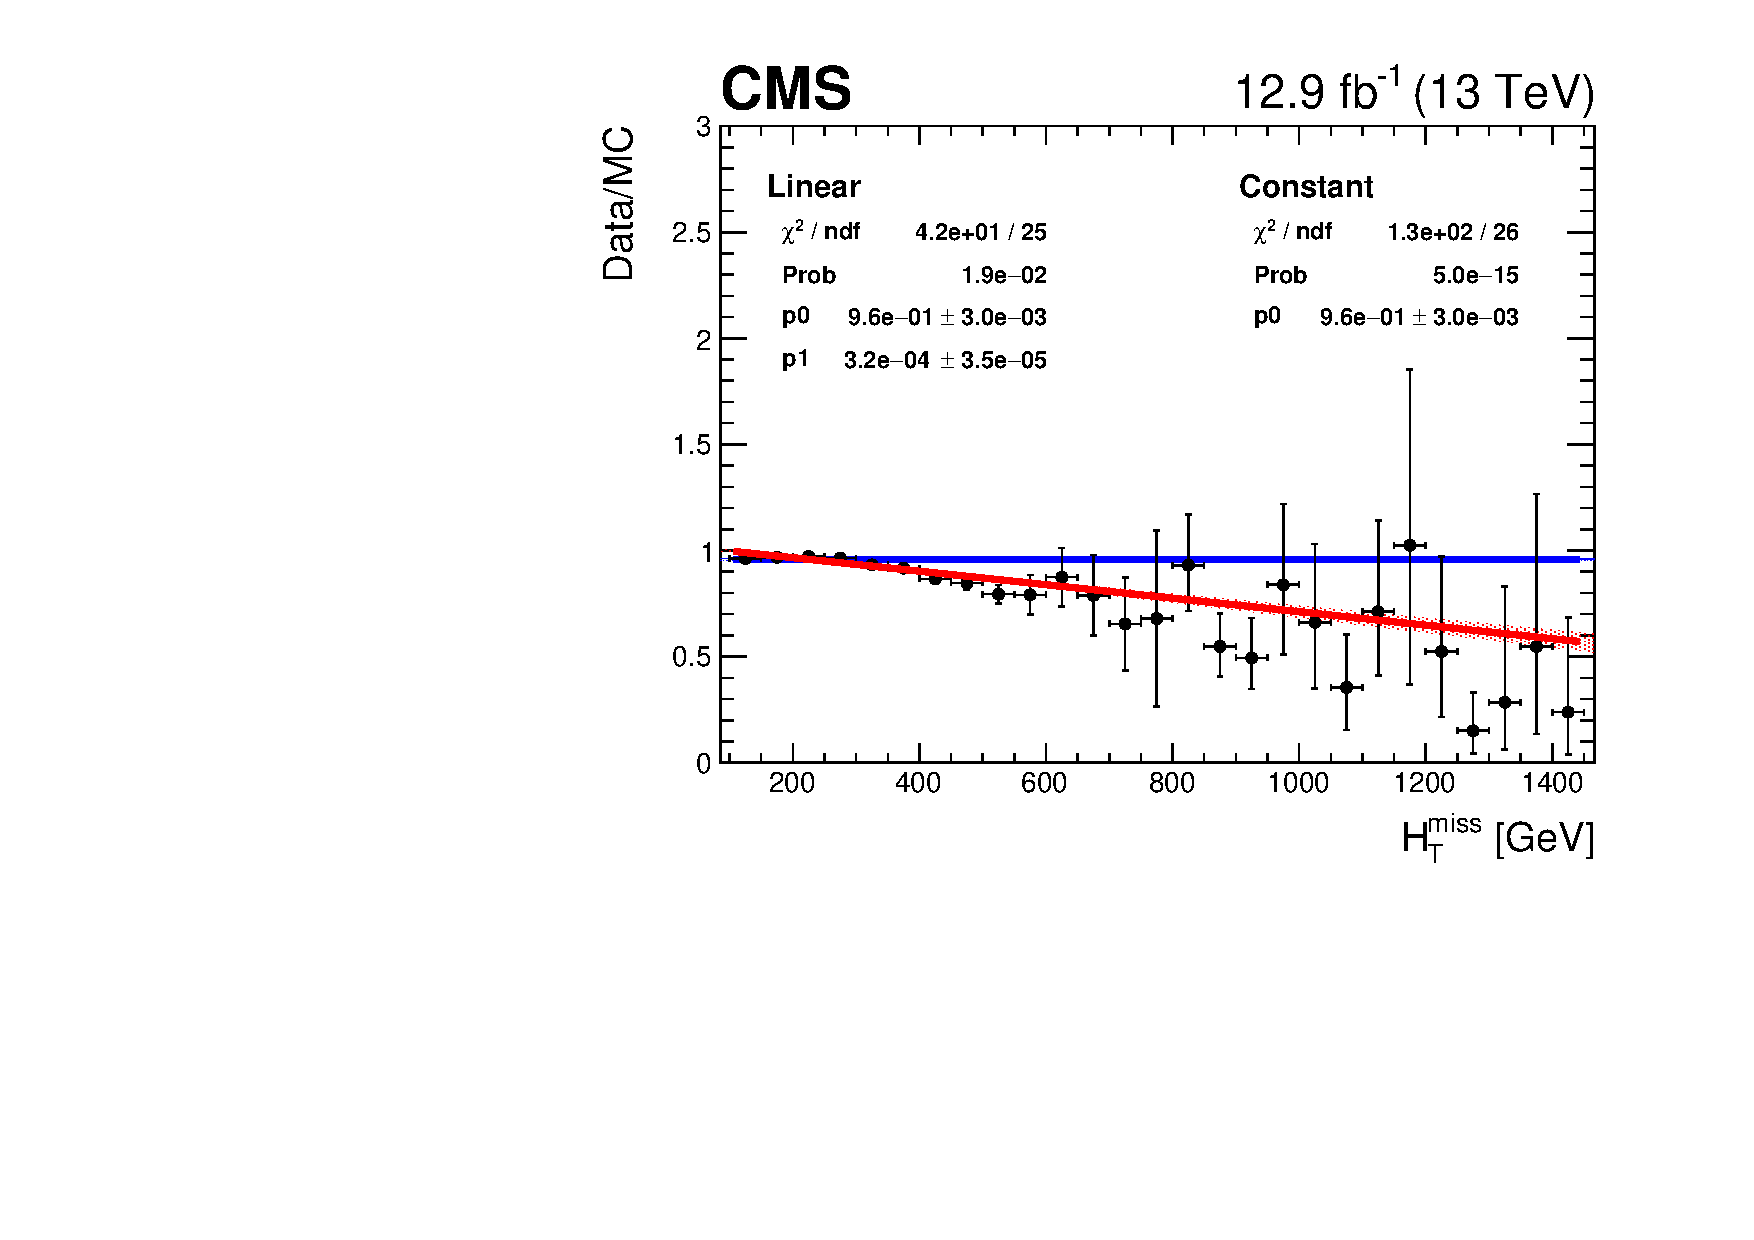
\includegraphics[width=0.45\textwidth]{Figures/backgroundPrediction/shapeOutput12FbInc/scale_ht_variable_mht/SingleMu/Inc_Inc/finalFits/mht_Inc_Inc_ht_Inc_SingleMu_Graph.pdf}
  }~~
  \subfloat[\gj]{
    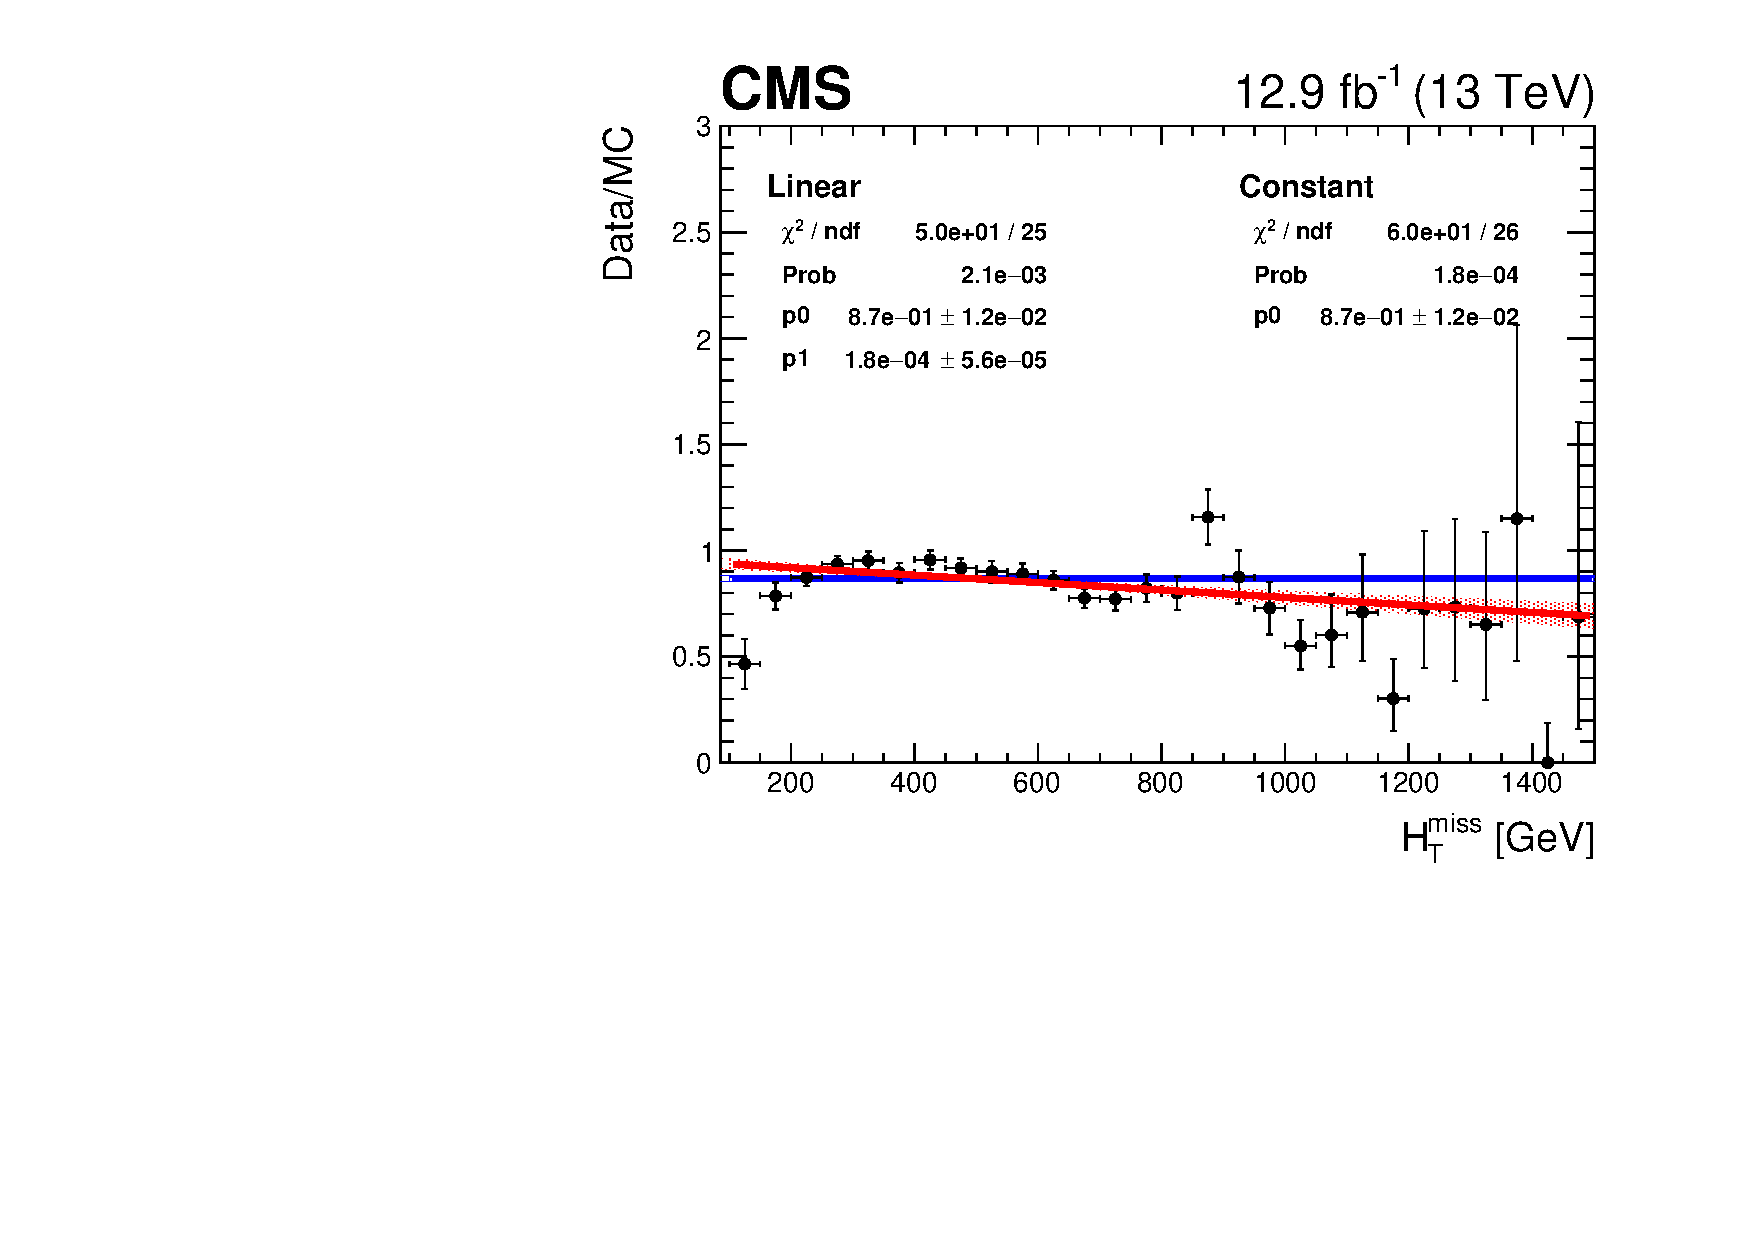
\includegraphics[width=0.45\textwidth]{Figures/backgroundPrediction/shapeOutput12FbInc/scale_ht_variable_mht/SinglePhoton/Inc_Inc/finalFits/mht_Inc_Inc_ht_Inc_SinglePhoton_Graph.pdf}
  }\\
  \subfloat[\mmj]{
    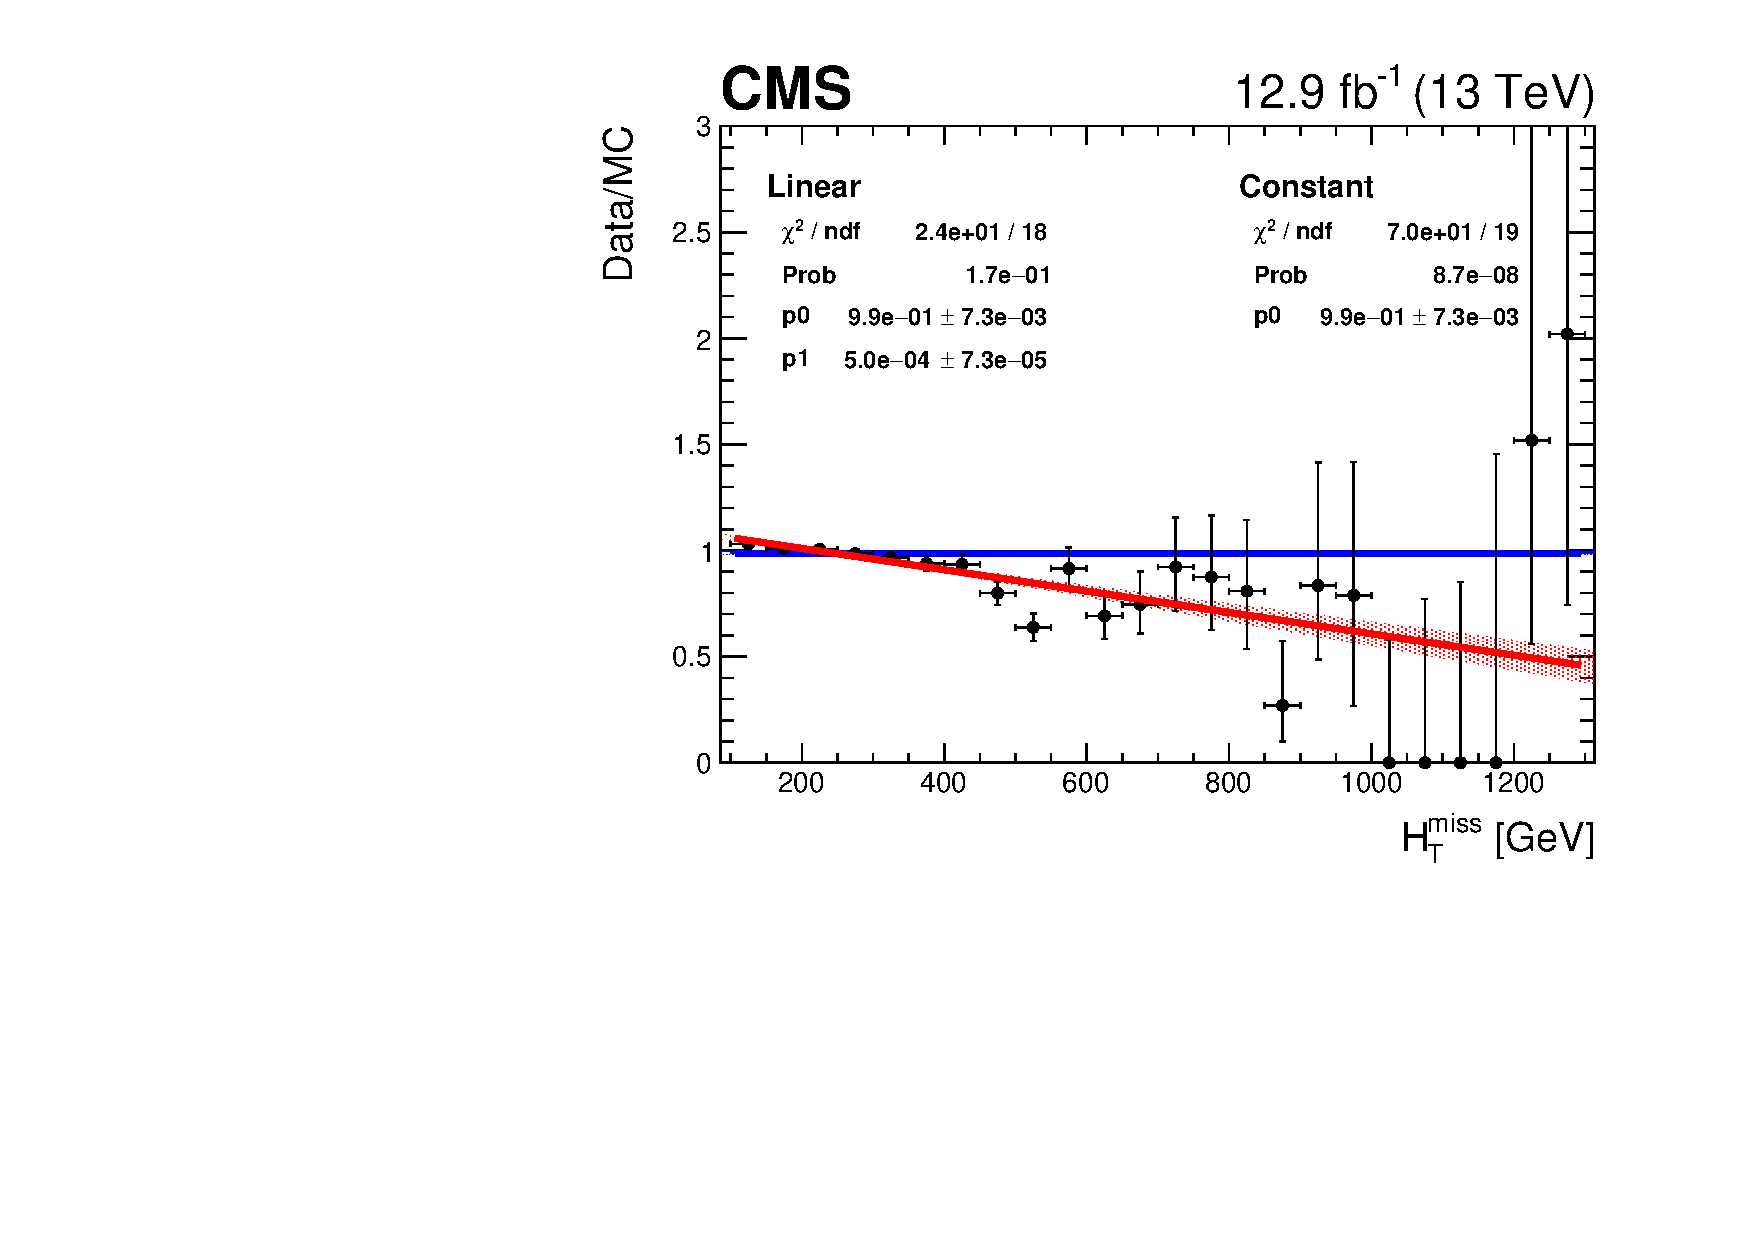
\includegraphics[width=0.45\textwidth]{Figures/backgroundPrediction/shapeOutput12FbInc/scale_ht_variable_mht/DoubleMu/Inc_Inc/finalFits/mht_Inc_Inc_ht_Inc_DoubleMu_Graph.pdf}
  }\\
  \caption{\label{fig:linearMotiv} 
  The data/simulation distribution against \mht~for an inclusive selection on category and \scalht
  showing the results of a linear fit. A large bias is observed as well as a low p-value for the constant fits. 
 }
\end{figure}

By binning in \scalht, \njet and \nb, the bias in the agreement 
between data and simulation due to mixing events at different scales is mitigated. 
In Figure~\ref{fig:linearFitExamples}, example fits of an linear OP to the data/simulation ratio 
are shown for the three control regions. Compared to the inclusive distribution
the linear component can be seen to be compatible with zero. In order to formalise this assertion,
the pull of the linear component from zero is calculated.
This pull distribution is shown for each of the three control regions 
in Figure~\ref{fig:pulls} and can be seen in each case to have a mean and sigma fairly 
consistent with zero and one, respectively, corresponding to the zero bias hypothesis.
In Figure~\ref{fig:frenchFlagPulls}, the distribution of the pulls 
in jet category and \scalht~bins shows no significant trend across the phase space.
Finally, the linear fits to the data/simulation ratio additionally have a p-value following 
a uniform distribution between 0 and 1 as shown in Figure~\ref{fig:pValues}.

\begin{figure}[h!]
  \centering
  \subfloat[\gj, 1b, 2j category and \scalht 400-500\GeV bin]{
    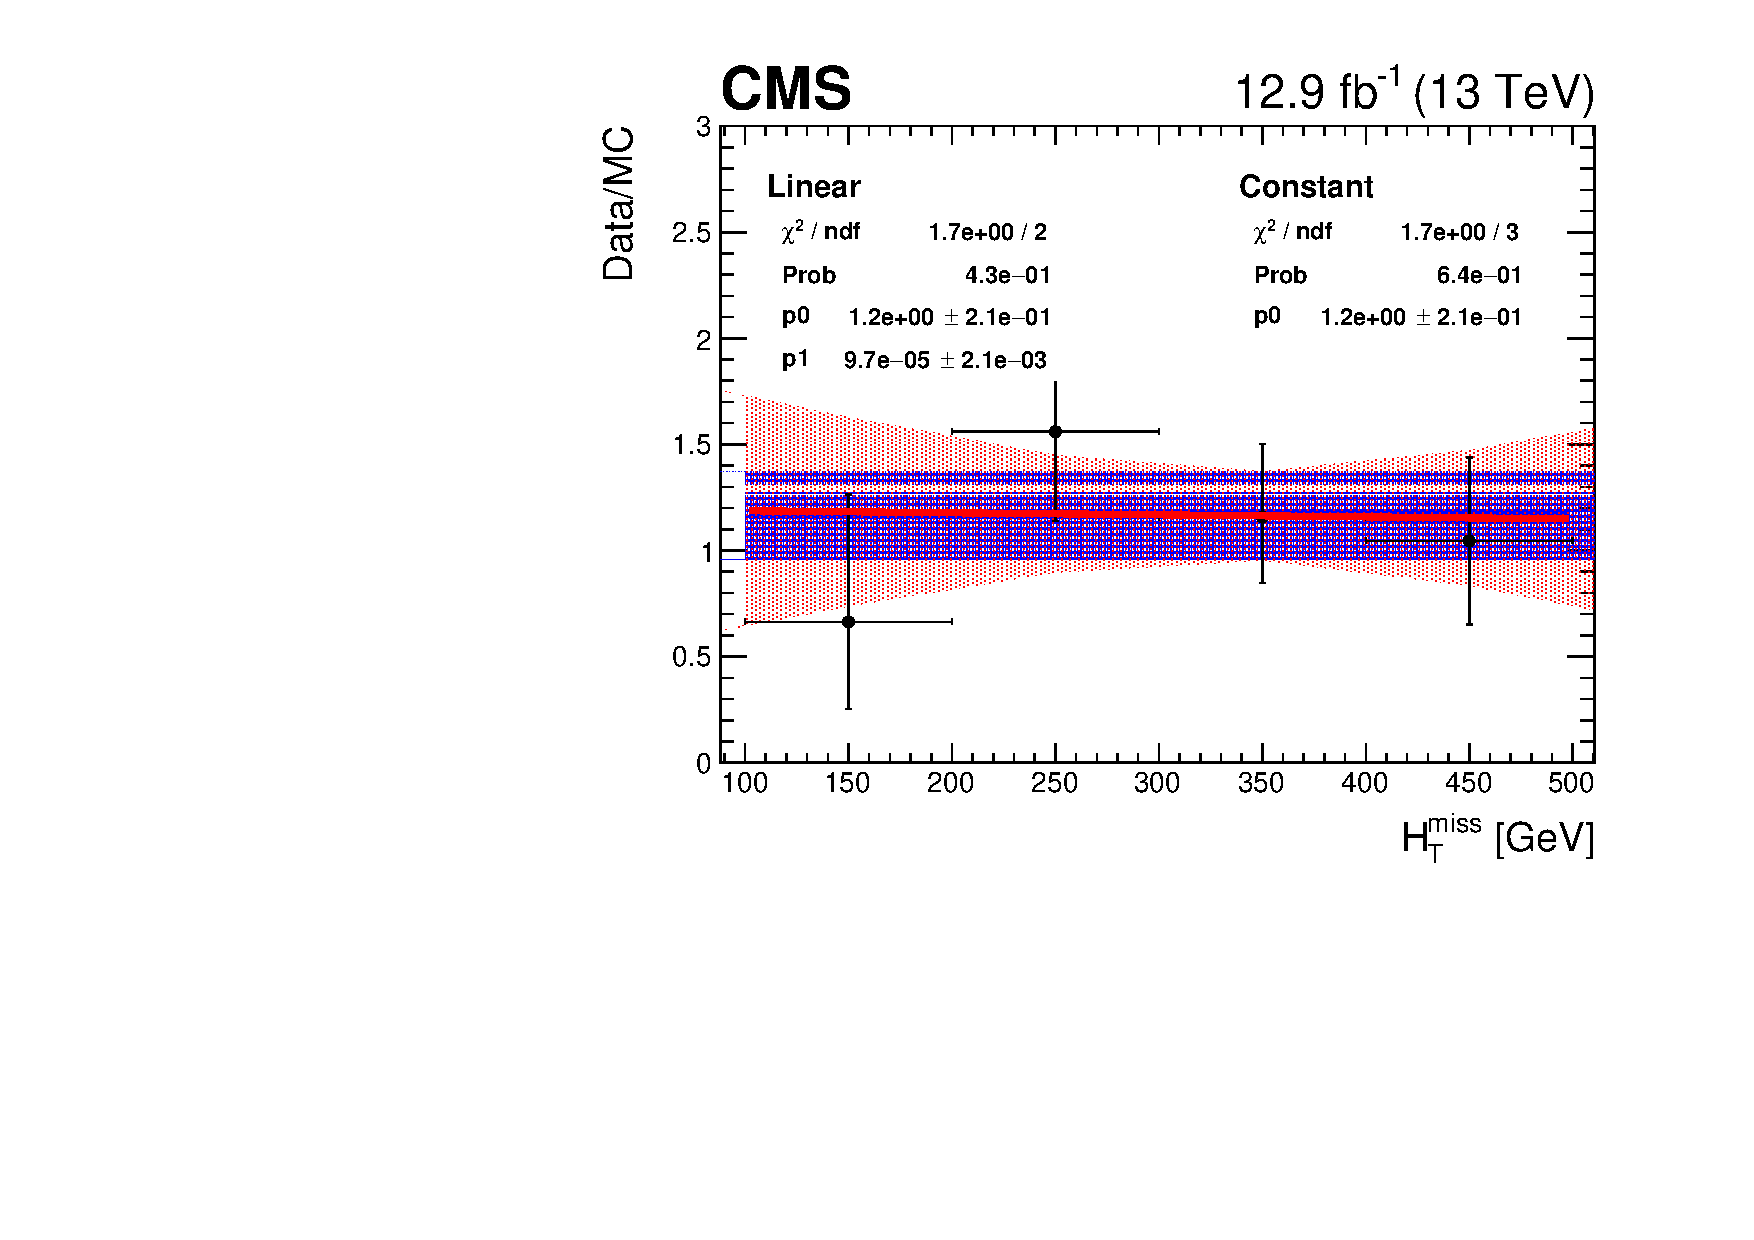
\includegraphics[width=0.45\textwidth]{Figures/backgroundPrediction/shapeOutput12Fb/scale_ht_variable_mht/representativeFits/mht_eq1b_eq2j_ht_400_500_SinglePhoton_Graph.pdf}
  }~~
  \subfloat[\mj, 1b, 4a category and \scalht 600-800\GeV bin]{
    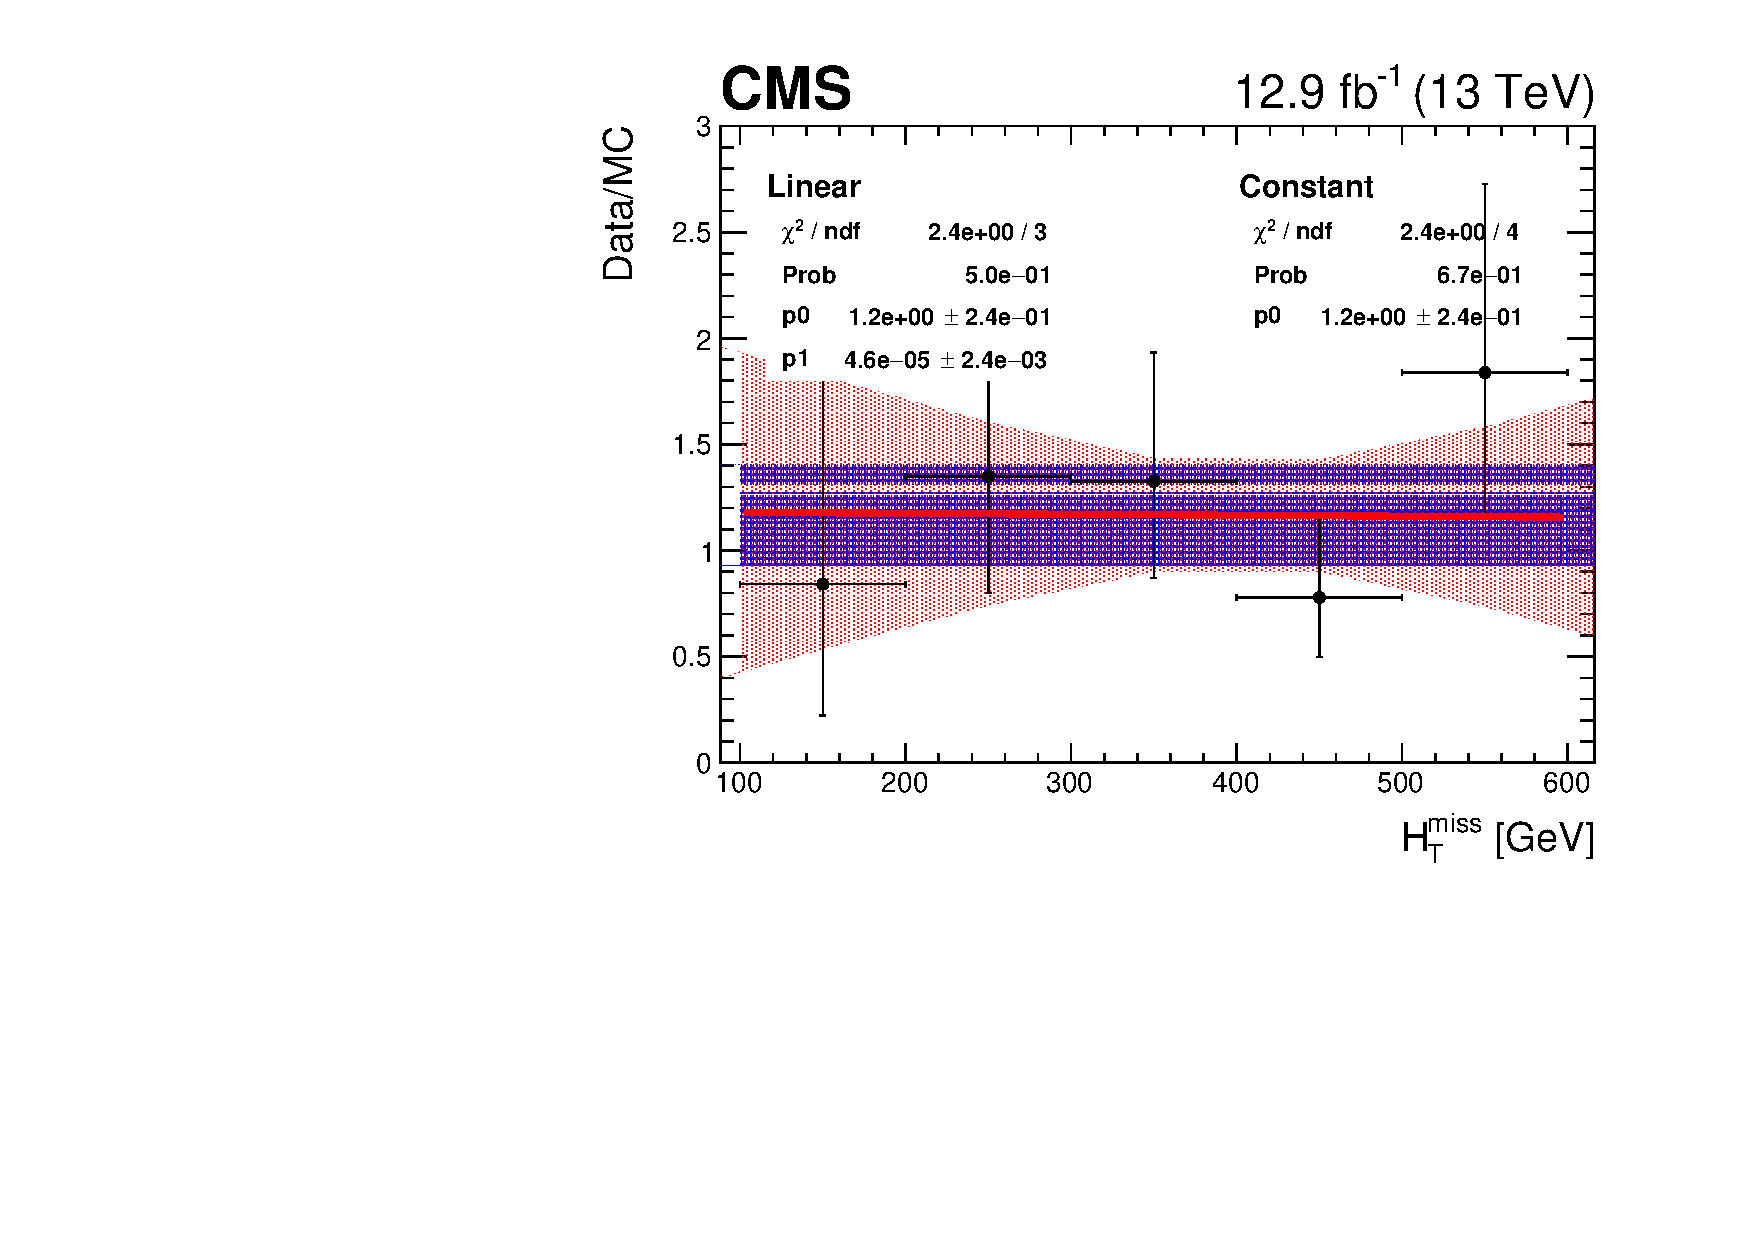
\includegraphics[width=0.45\textwidth]{Figures/backgroundPrediction/shapeOutput12Fb/scale_ht_variable_mht/representativeFits/mht_eq1b_eq4a_ht_600_800_SingleMu_Graph.pdf}
  }\\
  \subfloat[\mmj, 0b, 4j category and \scalht 300-350\GeV bin]{
    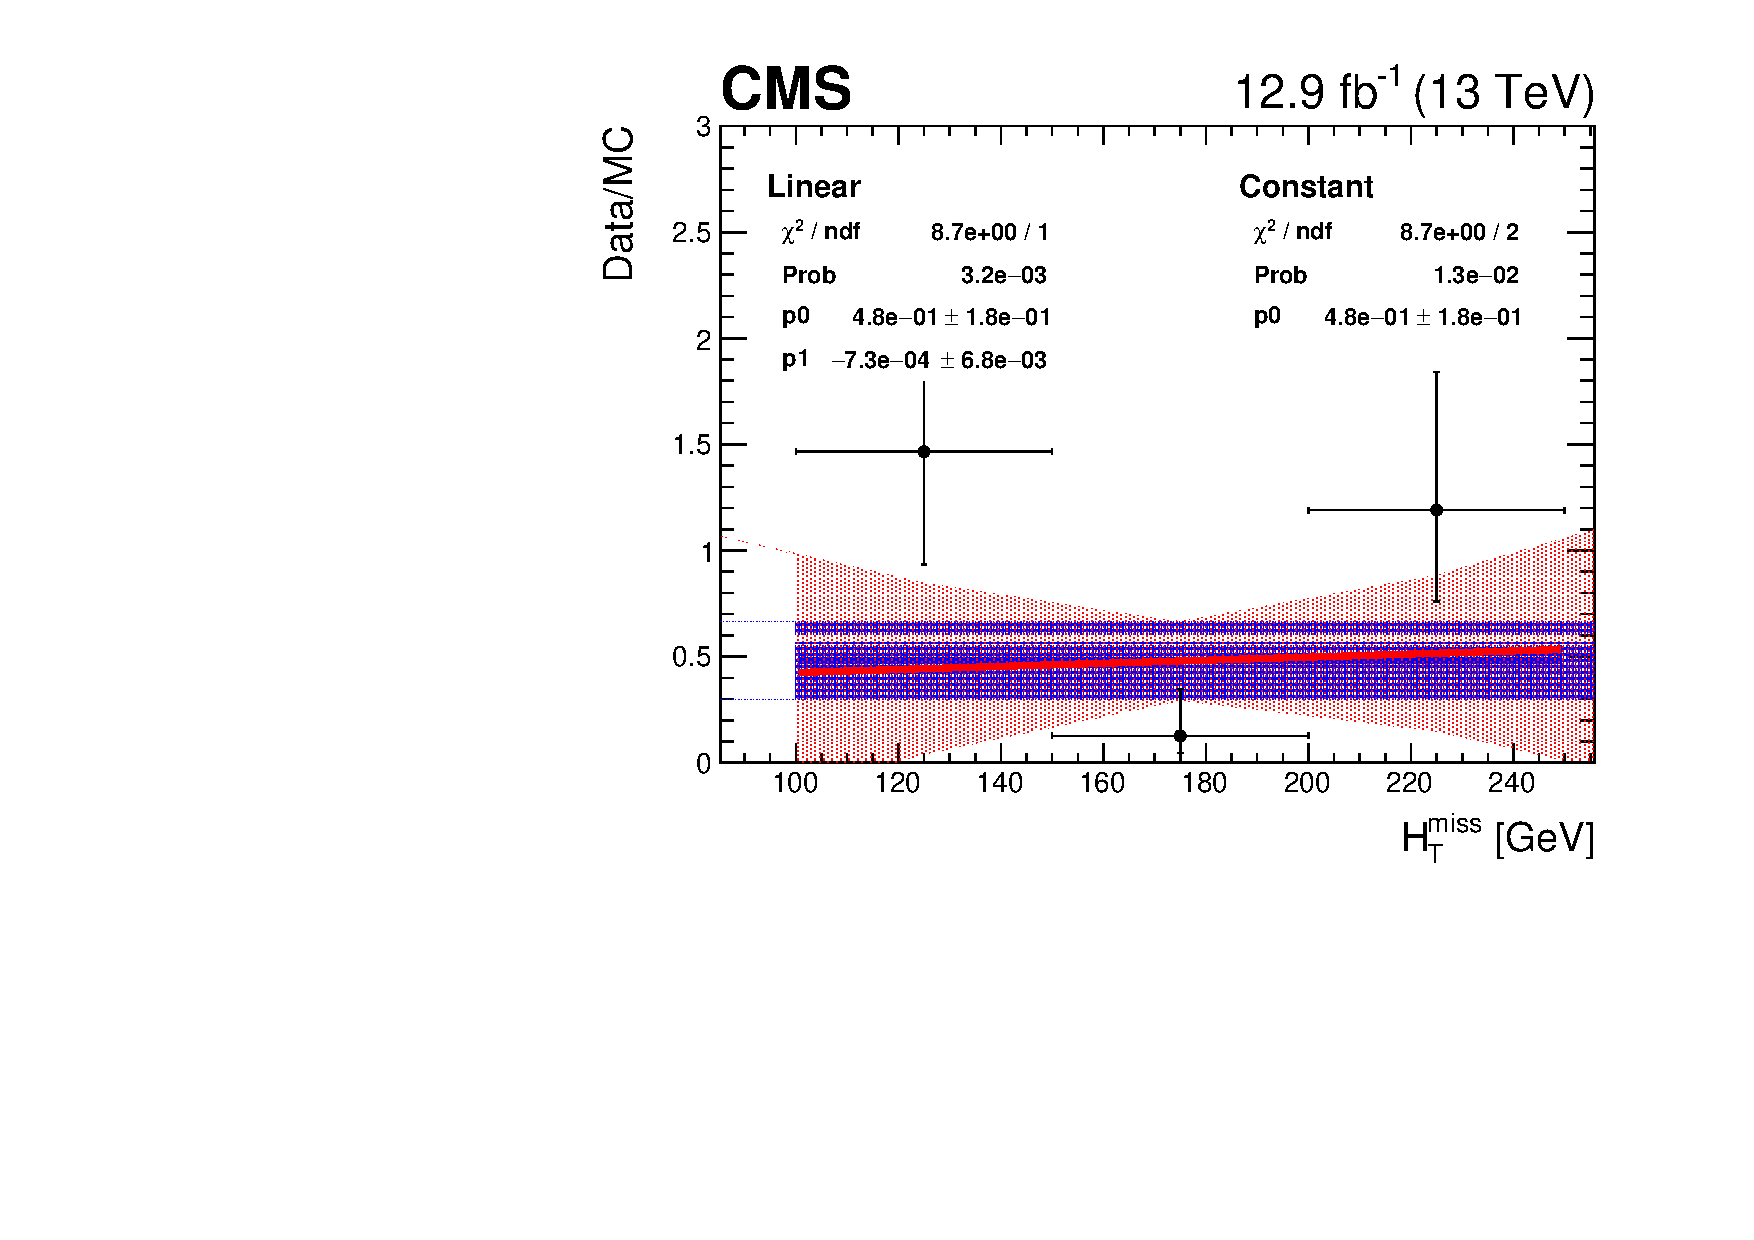
\includegraphics[width=0.45\textwidth]{Figures/backgroundPrediction/shapeOutput12Fb/scale_ht_variable_mht/representativeFits/mht_eq0b_eq4j_ht_300_350_DoubleMu_Graph.pdf}
  }~~
  \subfloat[\gj, 1b, 3j category and \scalht 600-800\GeV bin]{
    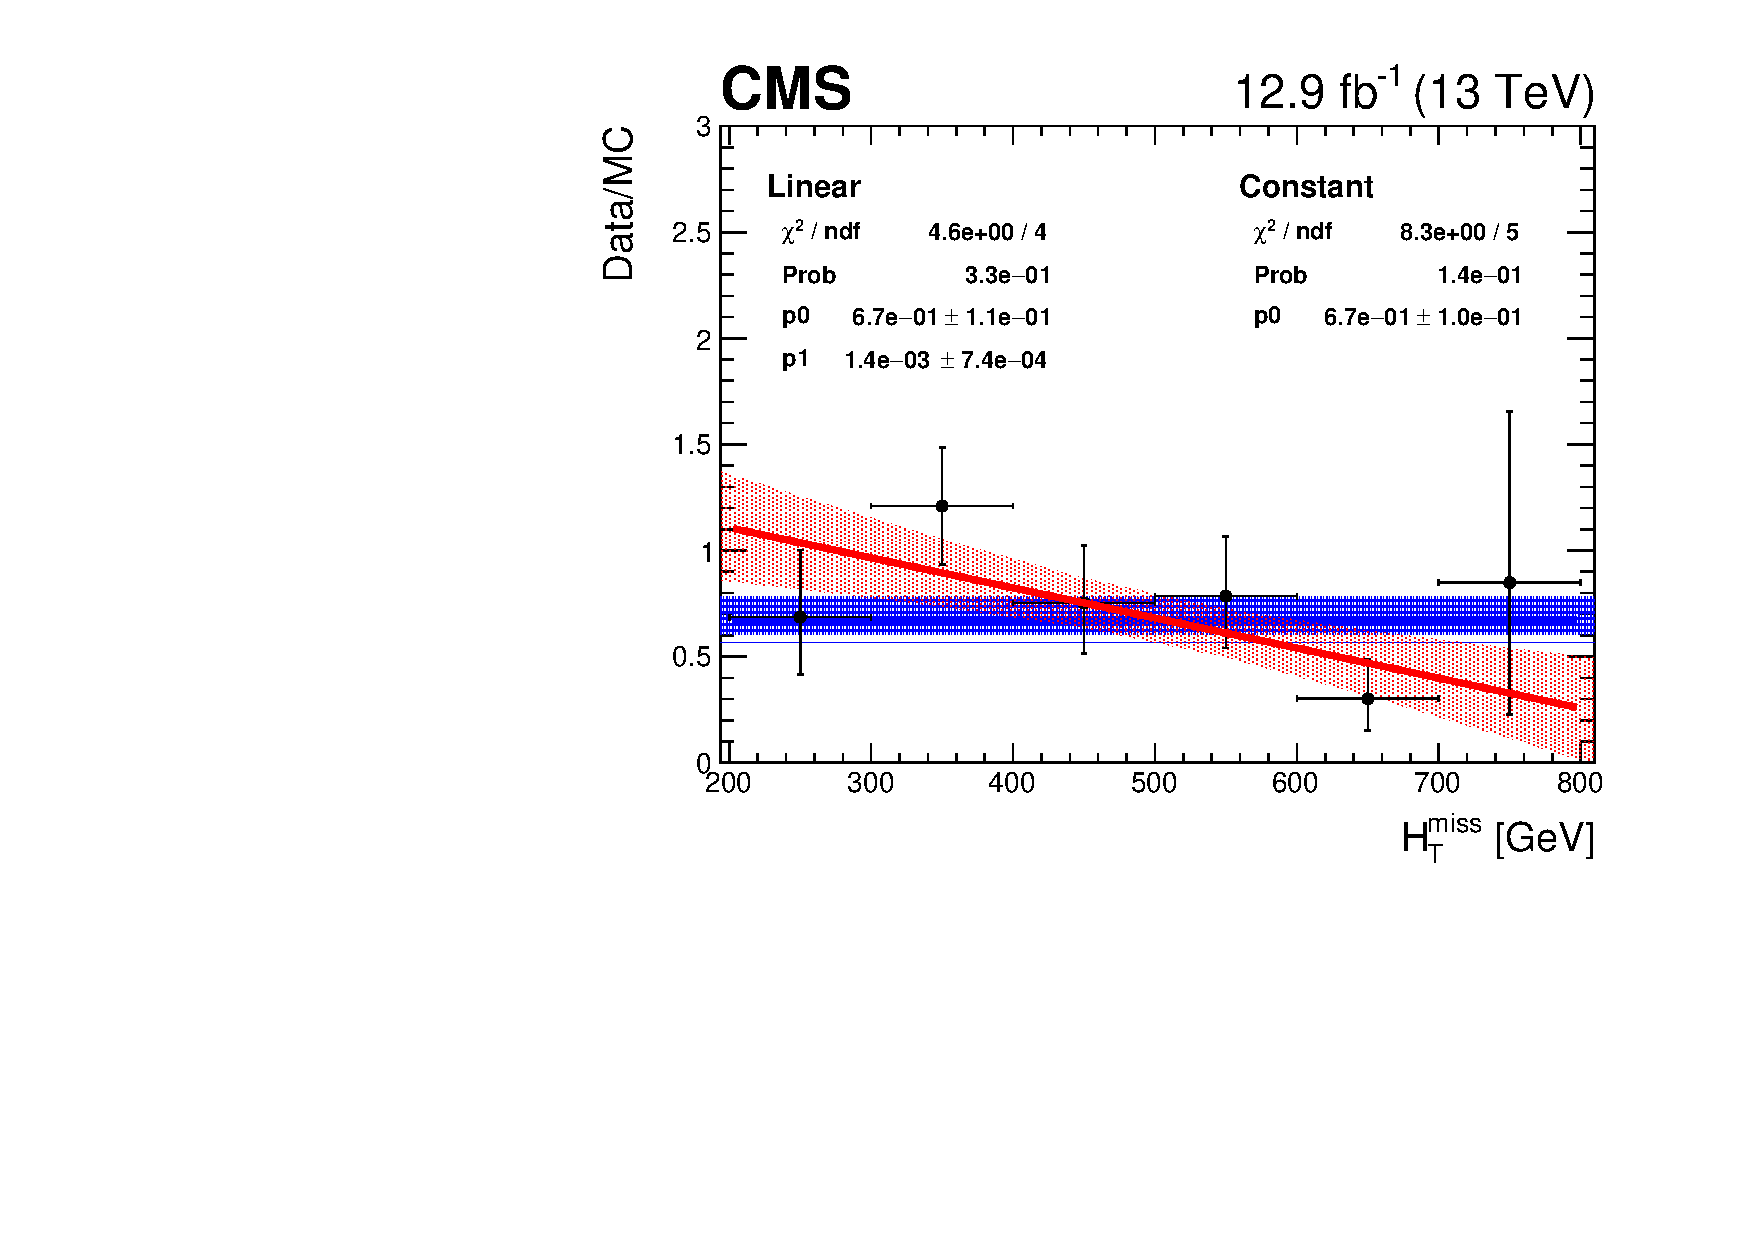
\includegraphics[width=0.45\textwidth]{Figures/backgroundPrediction/shapeOutput12Fb/scale_ht_variable_mht/SinglePhoton/eq1b_eq3j/finalFits/mht_eq1b_eq3j_ht_600_800_SinglePhoton_Graph.pdf}
  }\\
  \subfloat[\mj, 2b, 4j category and \scalht 600-800\GeV bin]{
    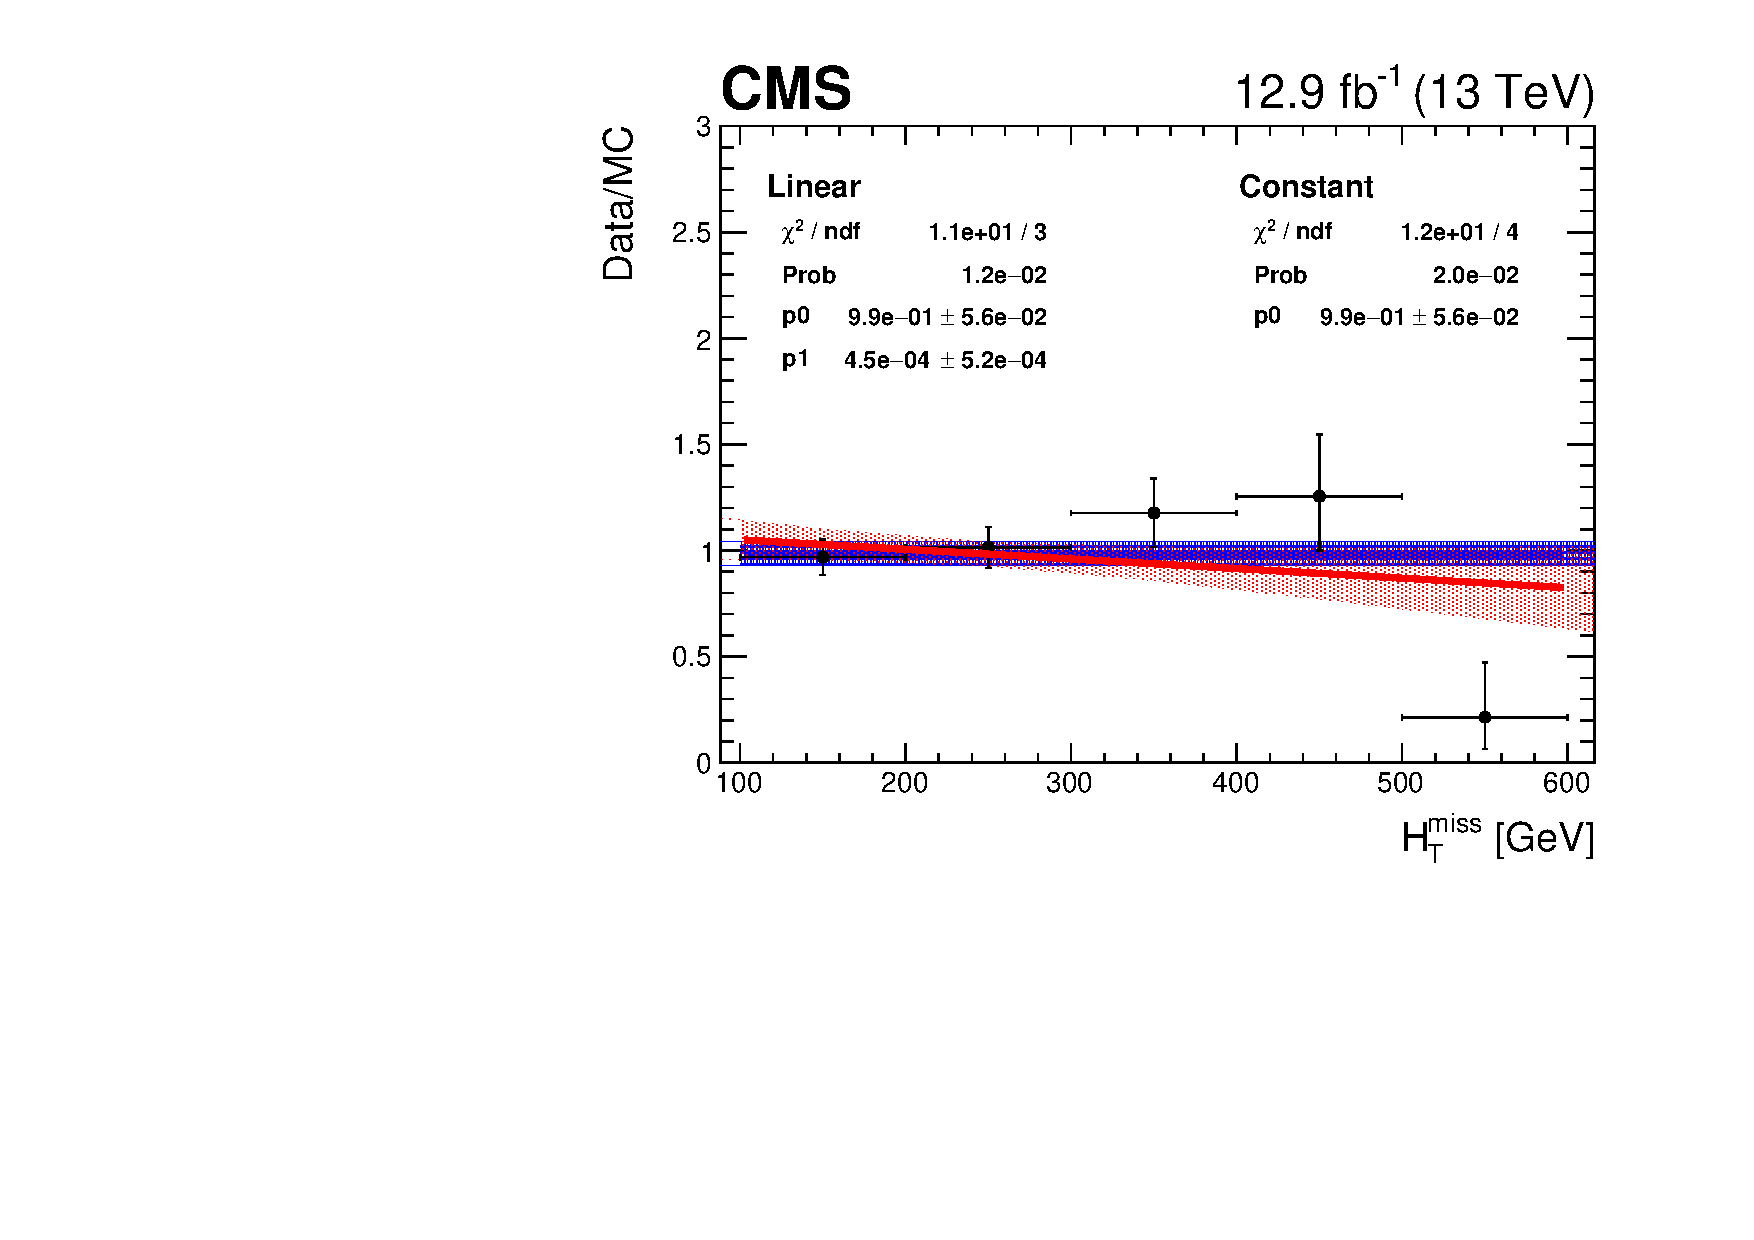
\includegraphics[width=0.45\textwidth]{Figures/backgroundPrediction/shapeOutput12Fb/scale_ht_variable_mht/SingleMu/eq2b_eq4j/finalFits/mht_eq2b_eq4j_ht_600_800_SingleMu_Graph.pdf}
  }~~
  \subfloat[\mmj, 0b, 3a category and \scalht 300-350\GeV bin]{
    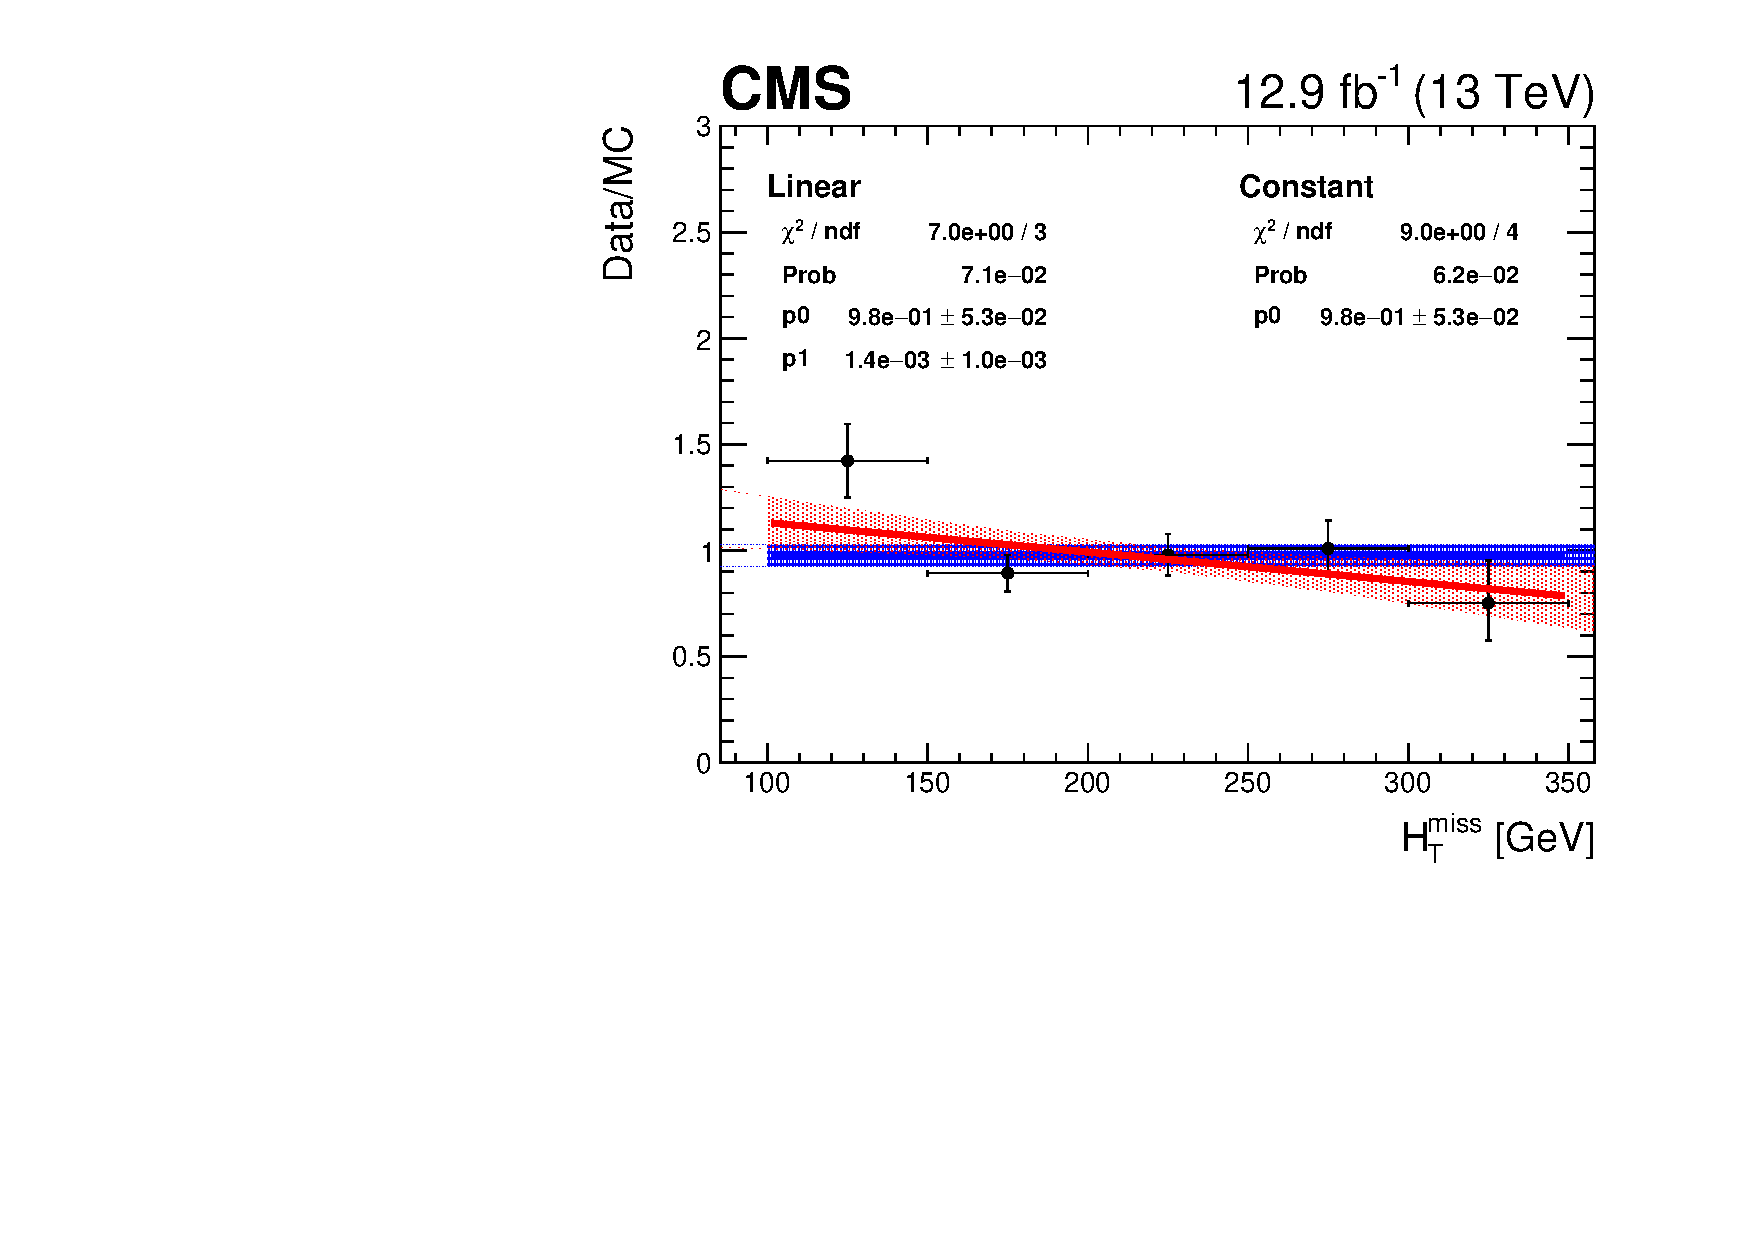
\includegraphics[width=0.45\textwidth]{Figures/backgroundPrediction/shapeOutput12Fb/scale_ht_variable_mht/DoubleMu/eq0b_eq3a/finalFits/mht_eq0b_eq3a_ht_300_350_DoubleMu_Graph.pdf}
  }\\
  \caption{\label{fig:linearFitExamples} 
  The data/simulation distribution against \mht~for example categories and control regions.
  The large bias in the linear component seen in Figure~\ref{fig:linearMotiv} is mitigated.}
\end{figure}

\begin{figure}[h!]
  \centering
  \subfloat[\mj]{
    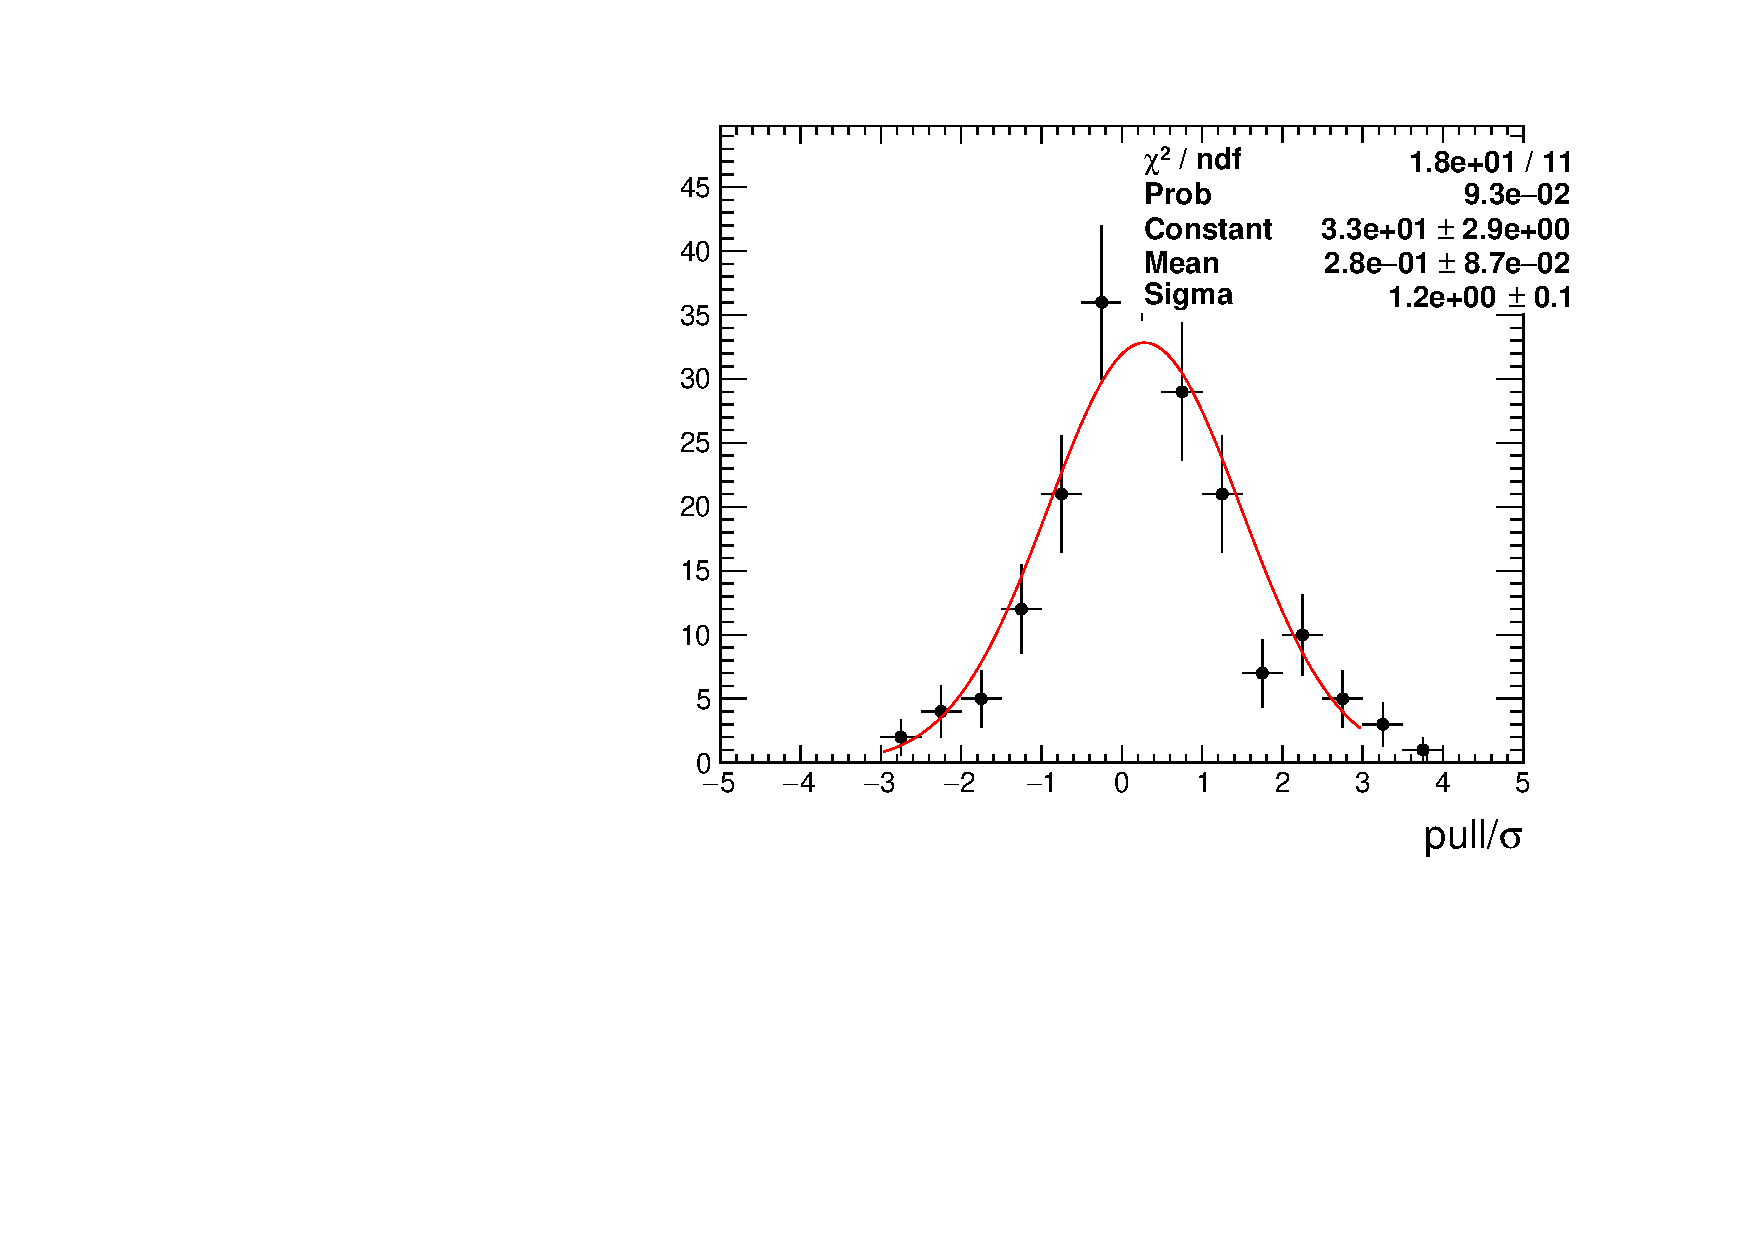
\includegraphics[width=0.45\textwidth]{Figures/backgroundPrediction/shapeOutput12Fb/scale_ht_variable_mht/SingleMu/fitOut/Linear2DShiftMean/pull_Linear2DShiftMean_p1_SingleMu.pdf}
  }~~
  \subfloat[\gj]{
    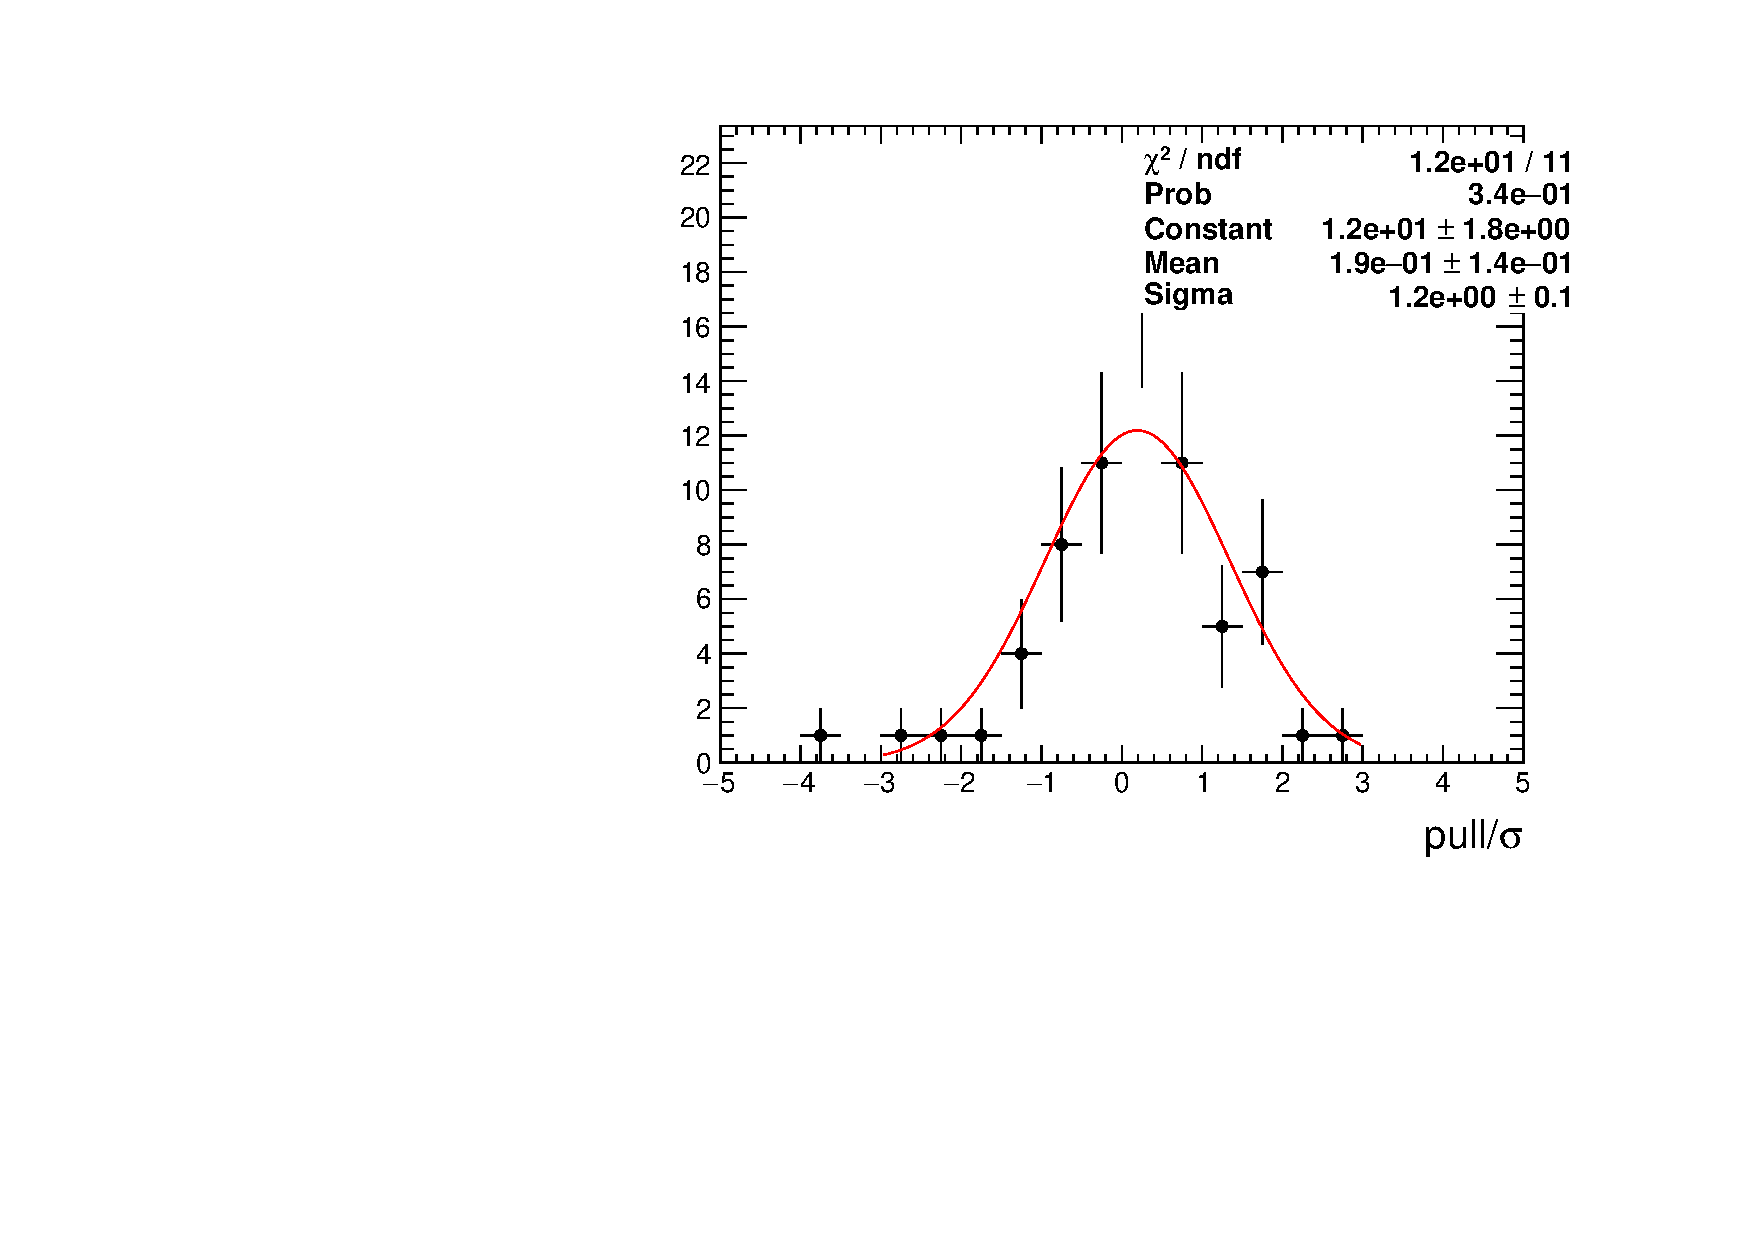
\includegraphics[width=0.45\textwidth]{Figures/backgroundPrediction/shapeOutput12Fb/scale_ht_variable_mht/SinglePhoton/fitOut/Linear2DShiftMean/pull_Linear2DShiftMean_p1_SinglePhoton.pdf}
  }\\
  \subfloat[\mmj]{
    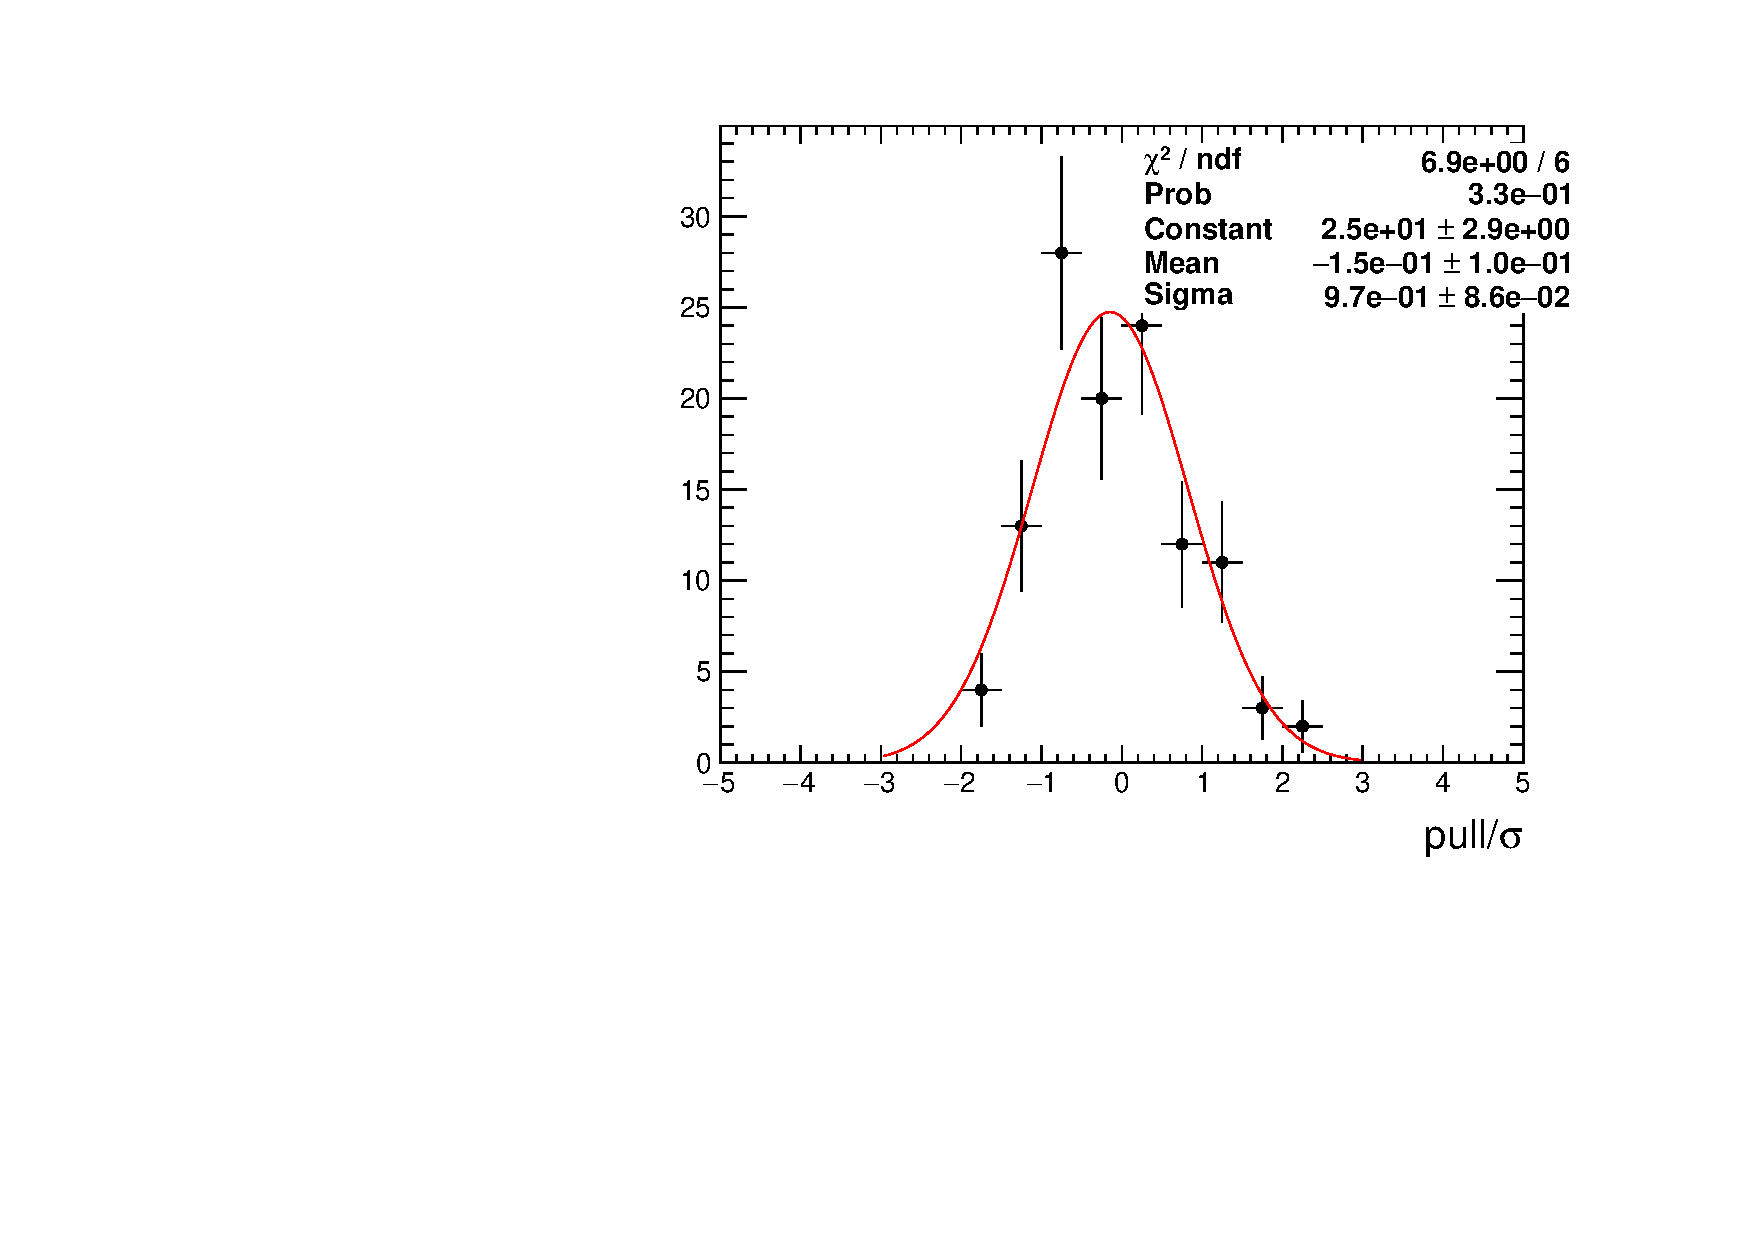
\includegraphics[width=0.45\textwidth]{Figures/backgroundPrediction/shapeOutput12Fb/scale_ht_variable_mht/DoubleMu/fitOut/Linear2DShiftMean/pull_Linear2DShiftMean_p1_DoubleMu.pdf}
  }~~
  \\
  \caption{\label{fig:pulls} 
  The pull distribution of the linear parameter from the flat hypothesis showing no significant bias.}
\end{figure}
\begin{figure}[h!]
  \centering
  \subfloat[\mj]{
    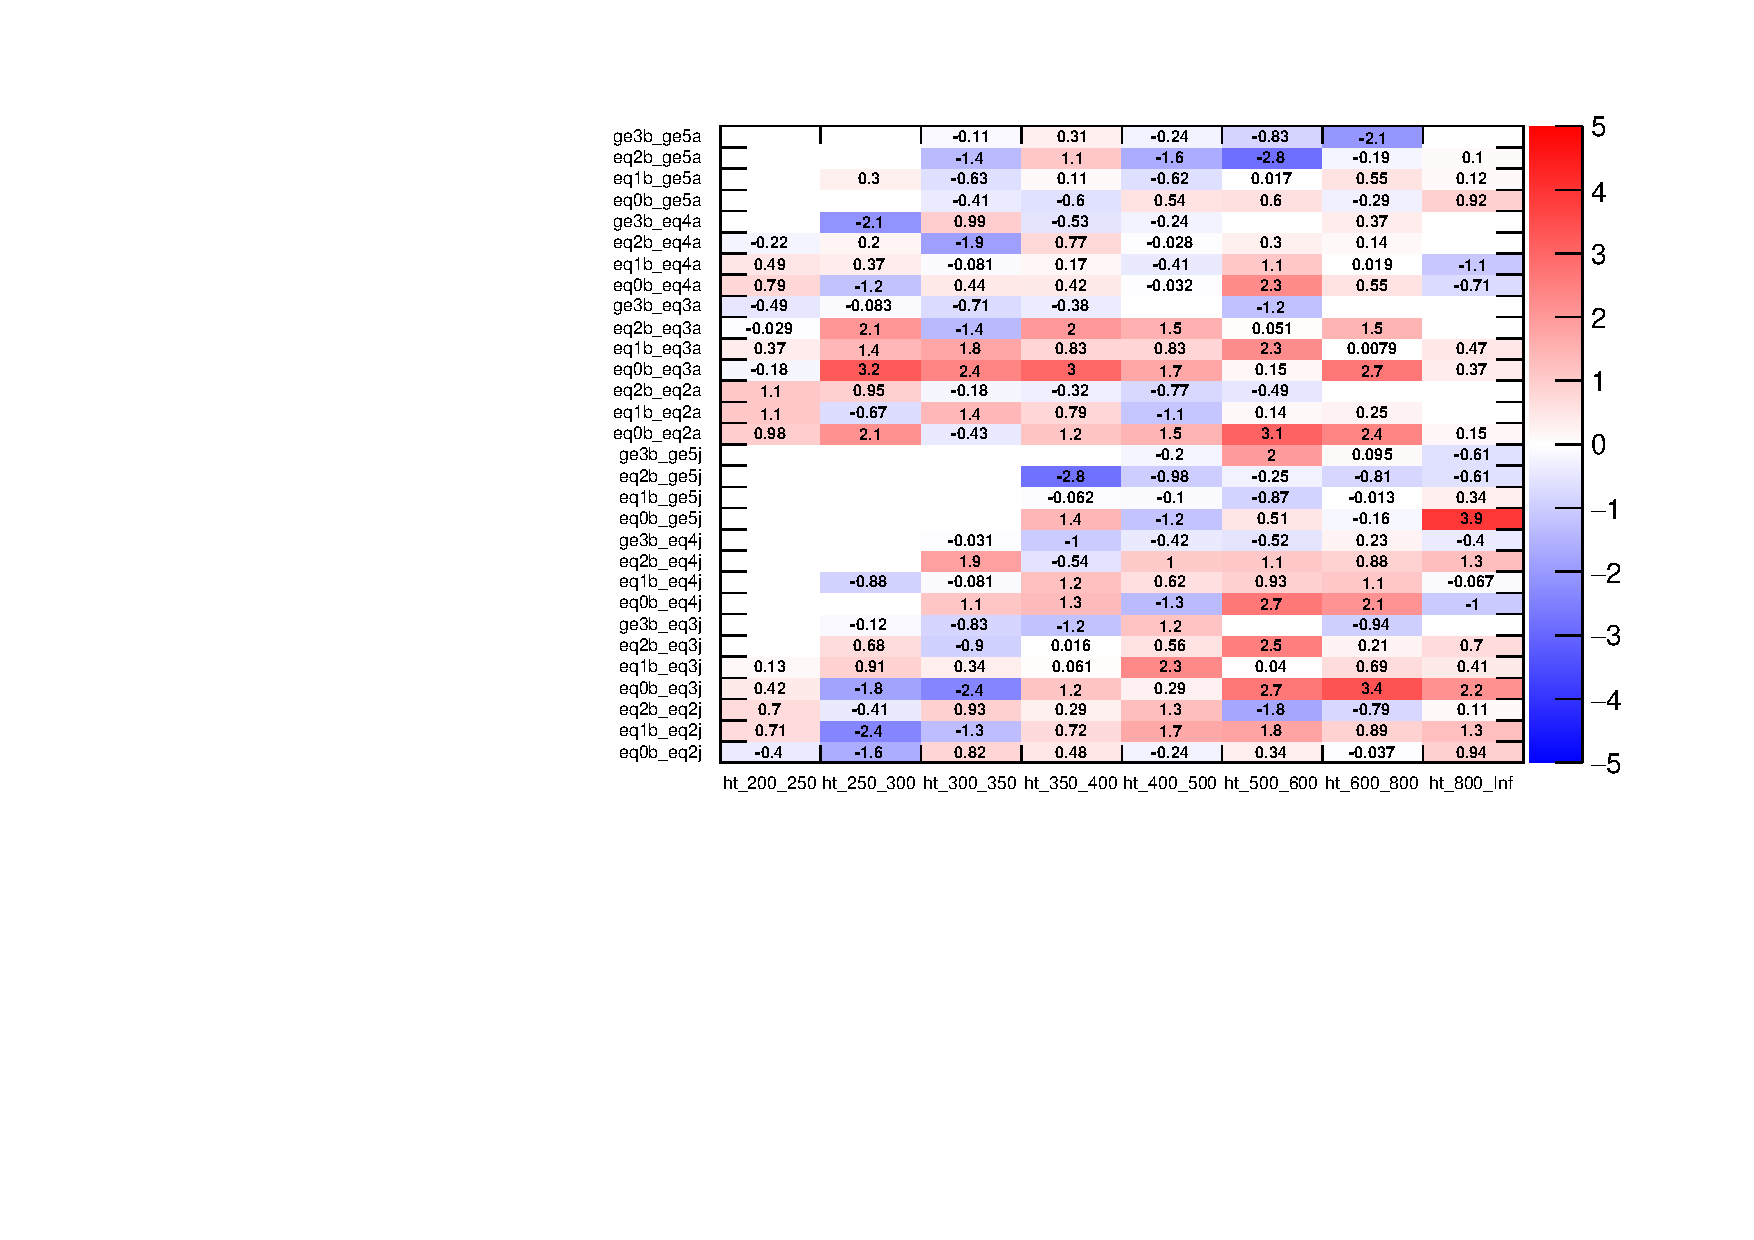
\includegraphics[width=0.45\textwidth]{Figures/backgroundPrediction/shapeOutput12Fb/scale_ht_variable_mht/SingleMu/fitOut/Linear2DShiftMean/frenchFlagPull_Linear2DShiftMean_p1_SingleMu.pdf}
  }~~
  \subfloat[\gj]{
    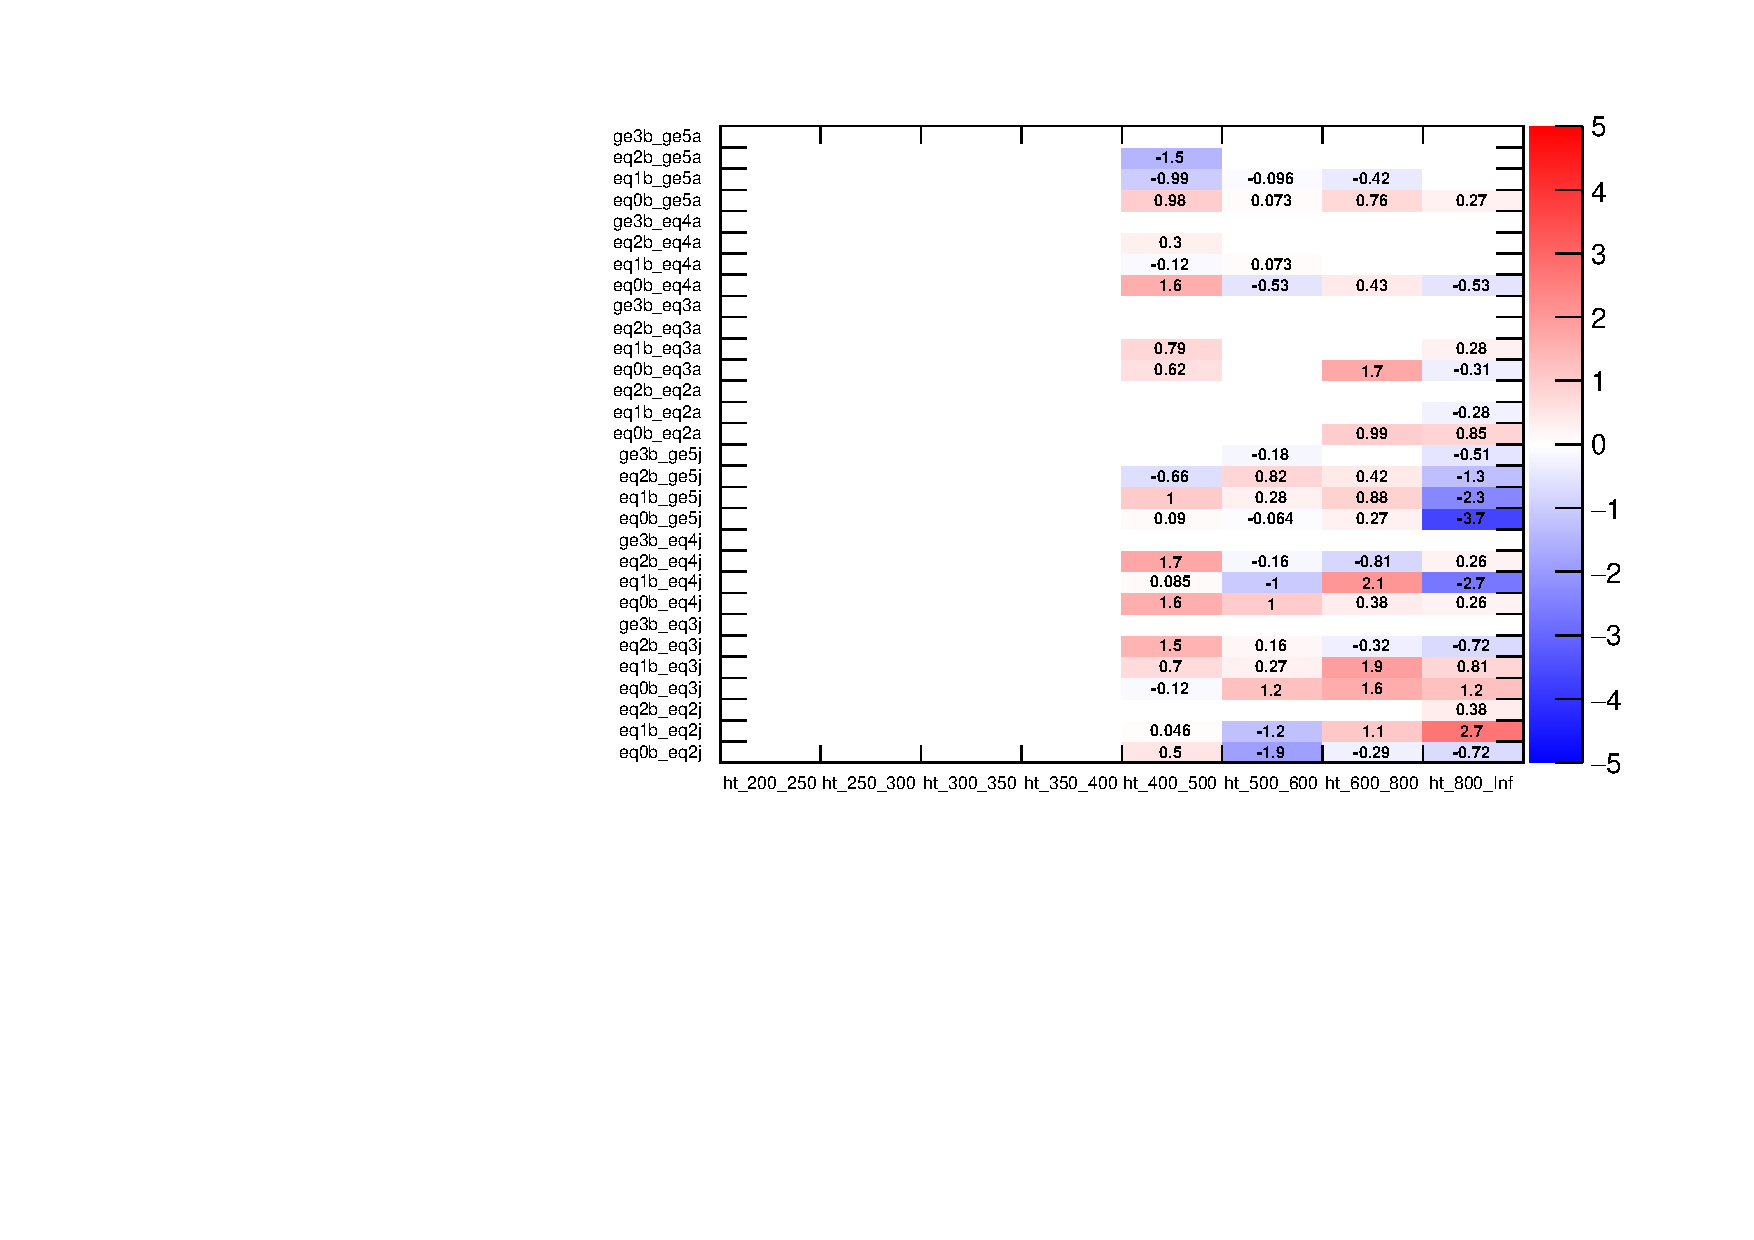
\includegraphics[width=0.45\textwidth]{Figures/backgroundPrediction/shapeOutput12Fb/scale_ht_variable_mht/SinglePhoton/fitOut/Linear2DShiftMean/frenchFlagPull_Linear2DShiftMean_p1_SinglePhoton.pdf}
  }\\
  \subfloat[\mmj]{
    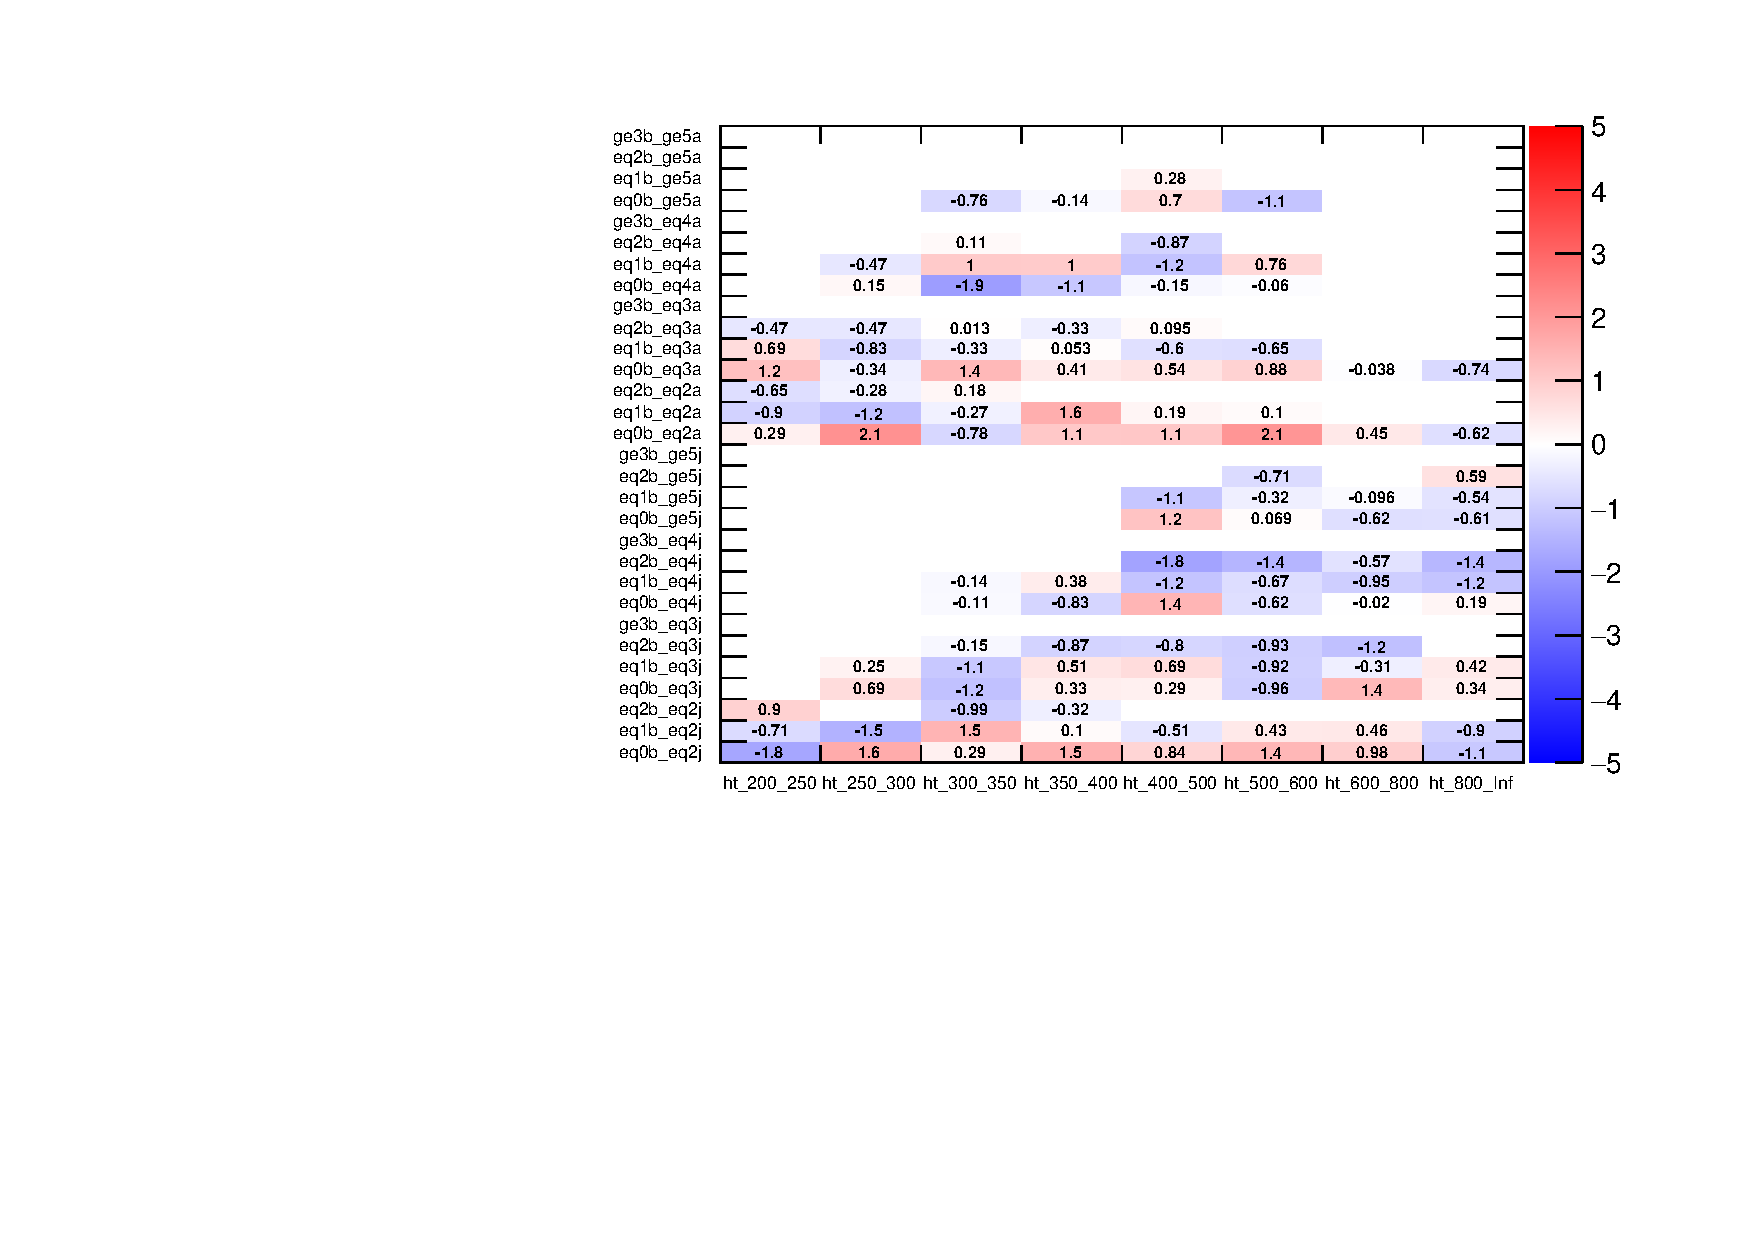
\includegraphics[width=0.45\textwidth]{Figures/backgroundPrediction/shapeOutput12Fb/scale_ht_variable_mht/DoubleMu/fitOut/Linear2DShiftMean/frenchFlagPull_Linear2DShiftMean_p1_DoubleMu.pdf}
  }~~
  \\
  \caption{\label{fig:frenchFlagPulls} The pull distribution of the linear parameter from the flat hypothesis across all
  \scalht~bins and categories. There are no significant pulls for the \scalht~binned
  fits while the \scalht~inclusive case shows very large pulls as expected.}
\end{figure}

\begin{figure}[h!]
  \centering
  \subfloat[\mj]{
    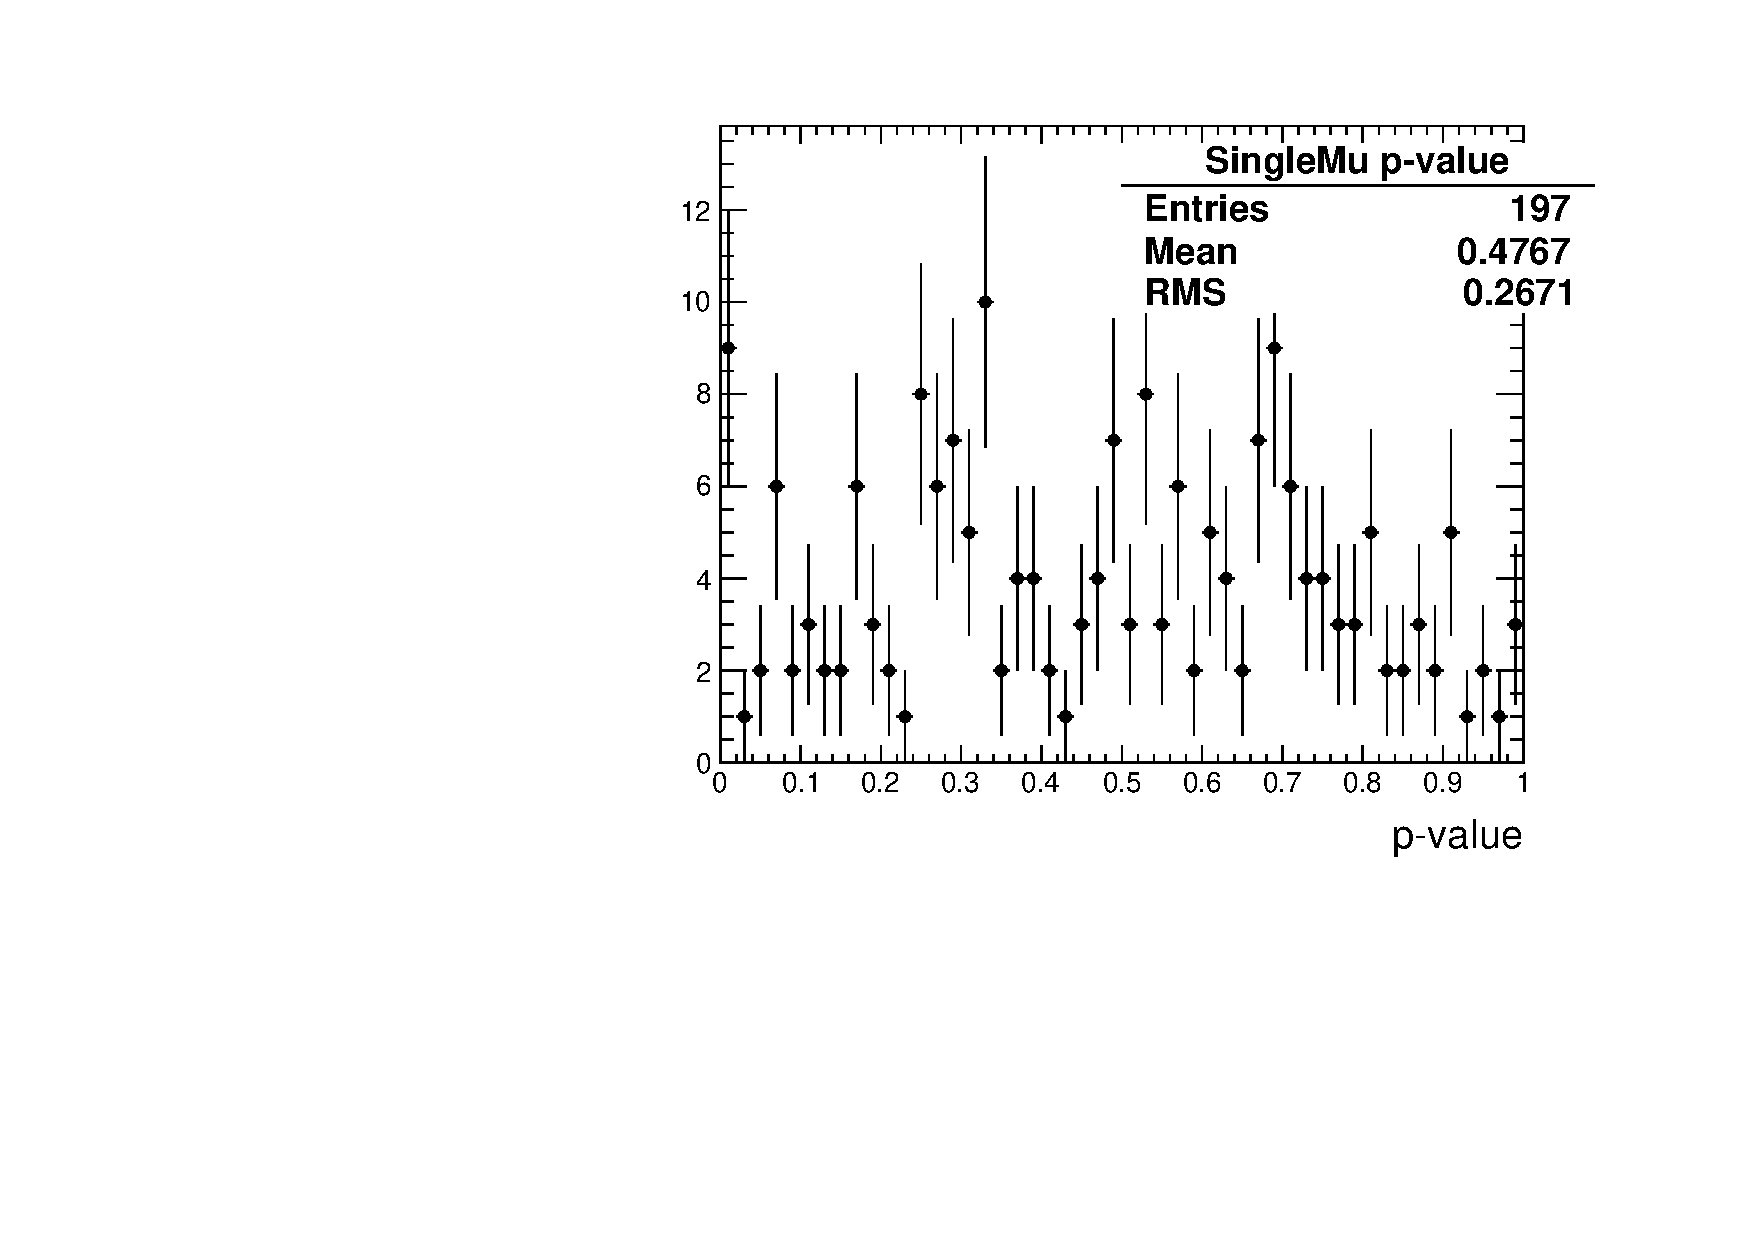
\includegraphics[width=0.45\textwidth]{Figures/backgroundPrediction/shapeOutput12Fb/scale_ht_variable_mht/SingleMu/fitOut/Linear2DShiftMean/pValue_Linear2DShiftMean_SingleMu.pdf}
  }~~
  \subfloat[\gj]{
    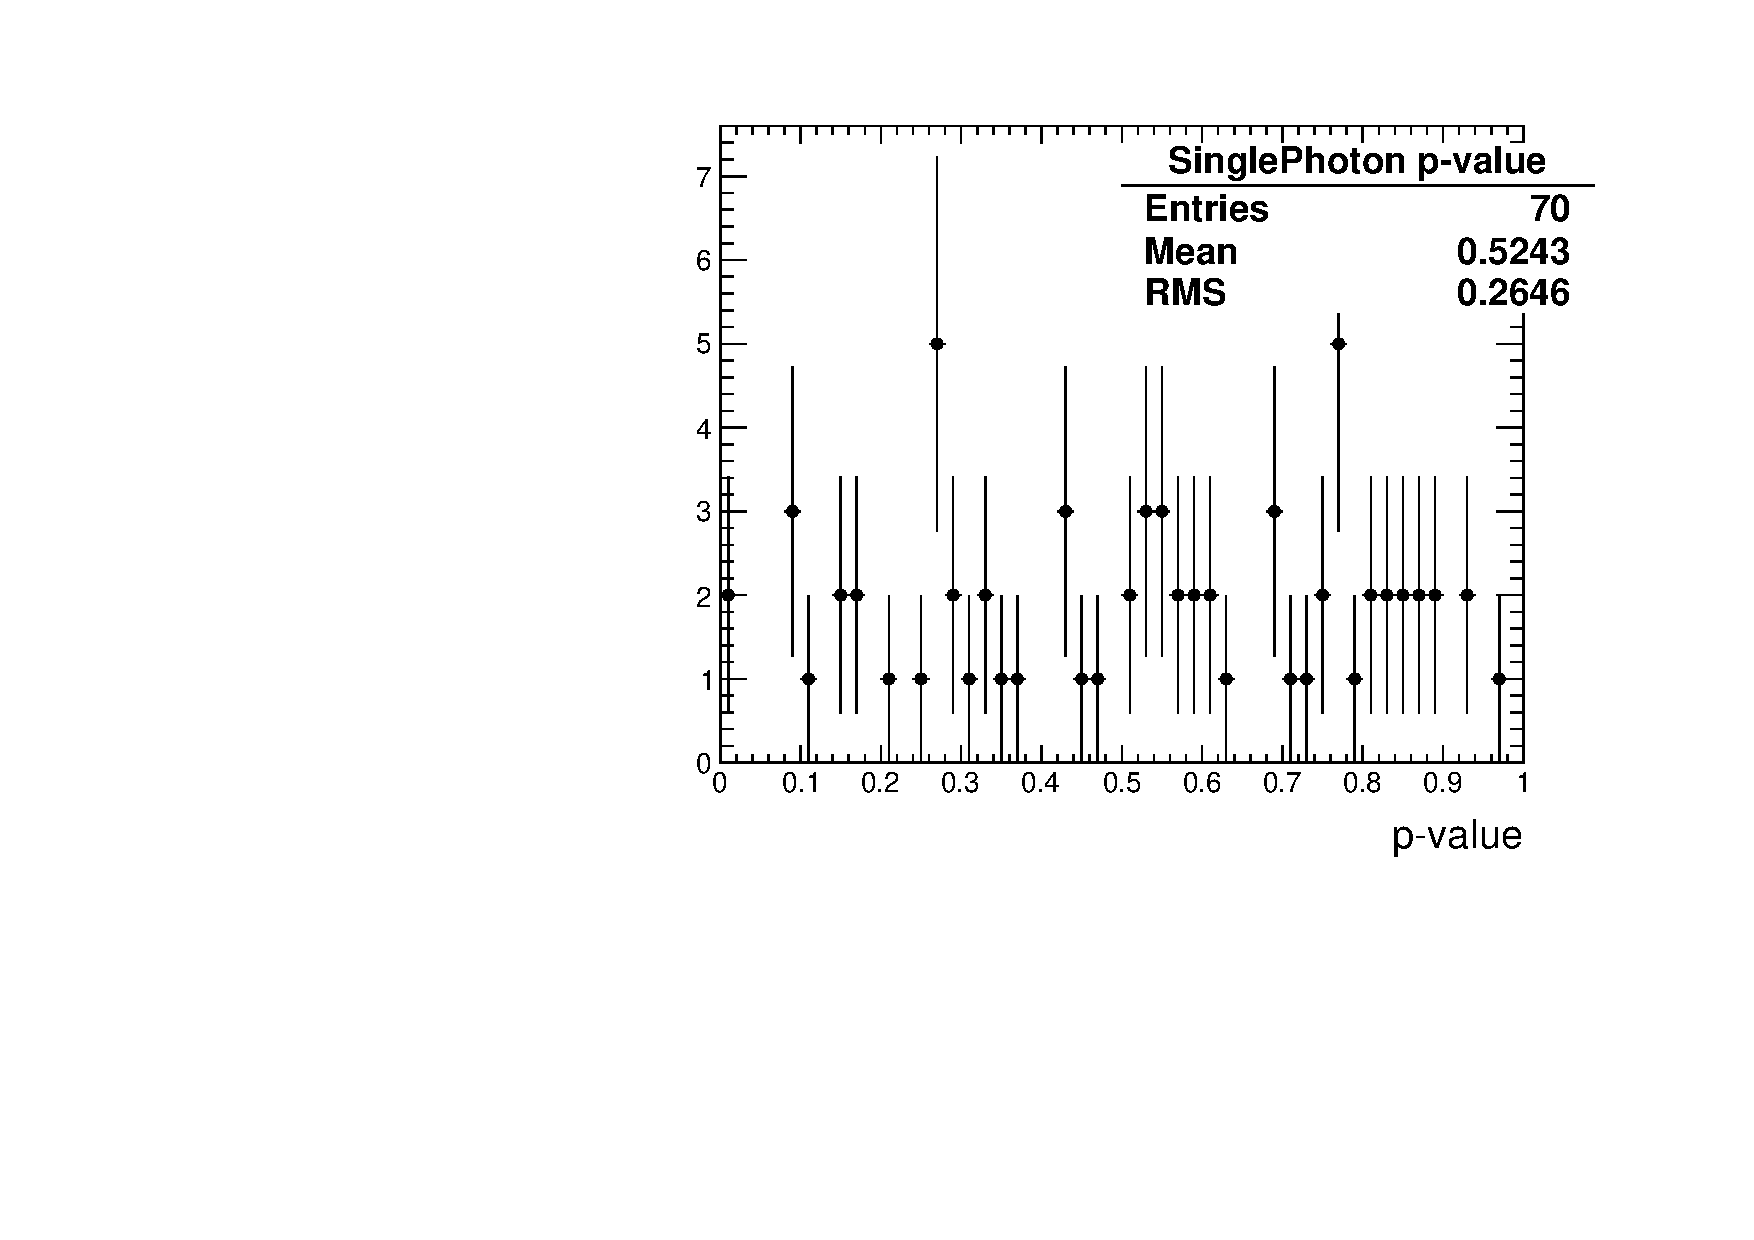
\includegraphics[width=0.45\textwidth]{Figures/backgroundPrediction/shapeOutput12Fb/scale_ht_variable_mht/SinglePhoton/fitOut/Linear2DShiftMean/pValue_Linear2DShiftMean_SinglePhoton.pdf}
  }\\
  \subfloat[\mmj]{
    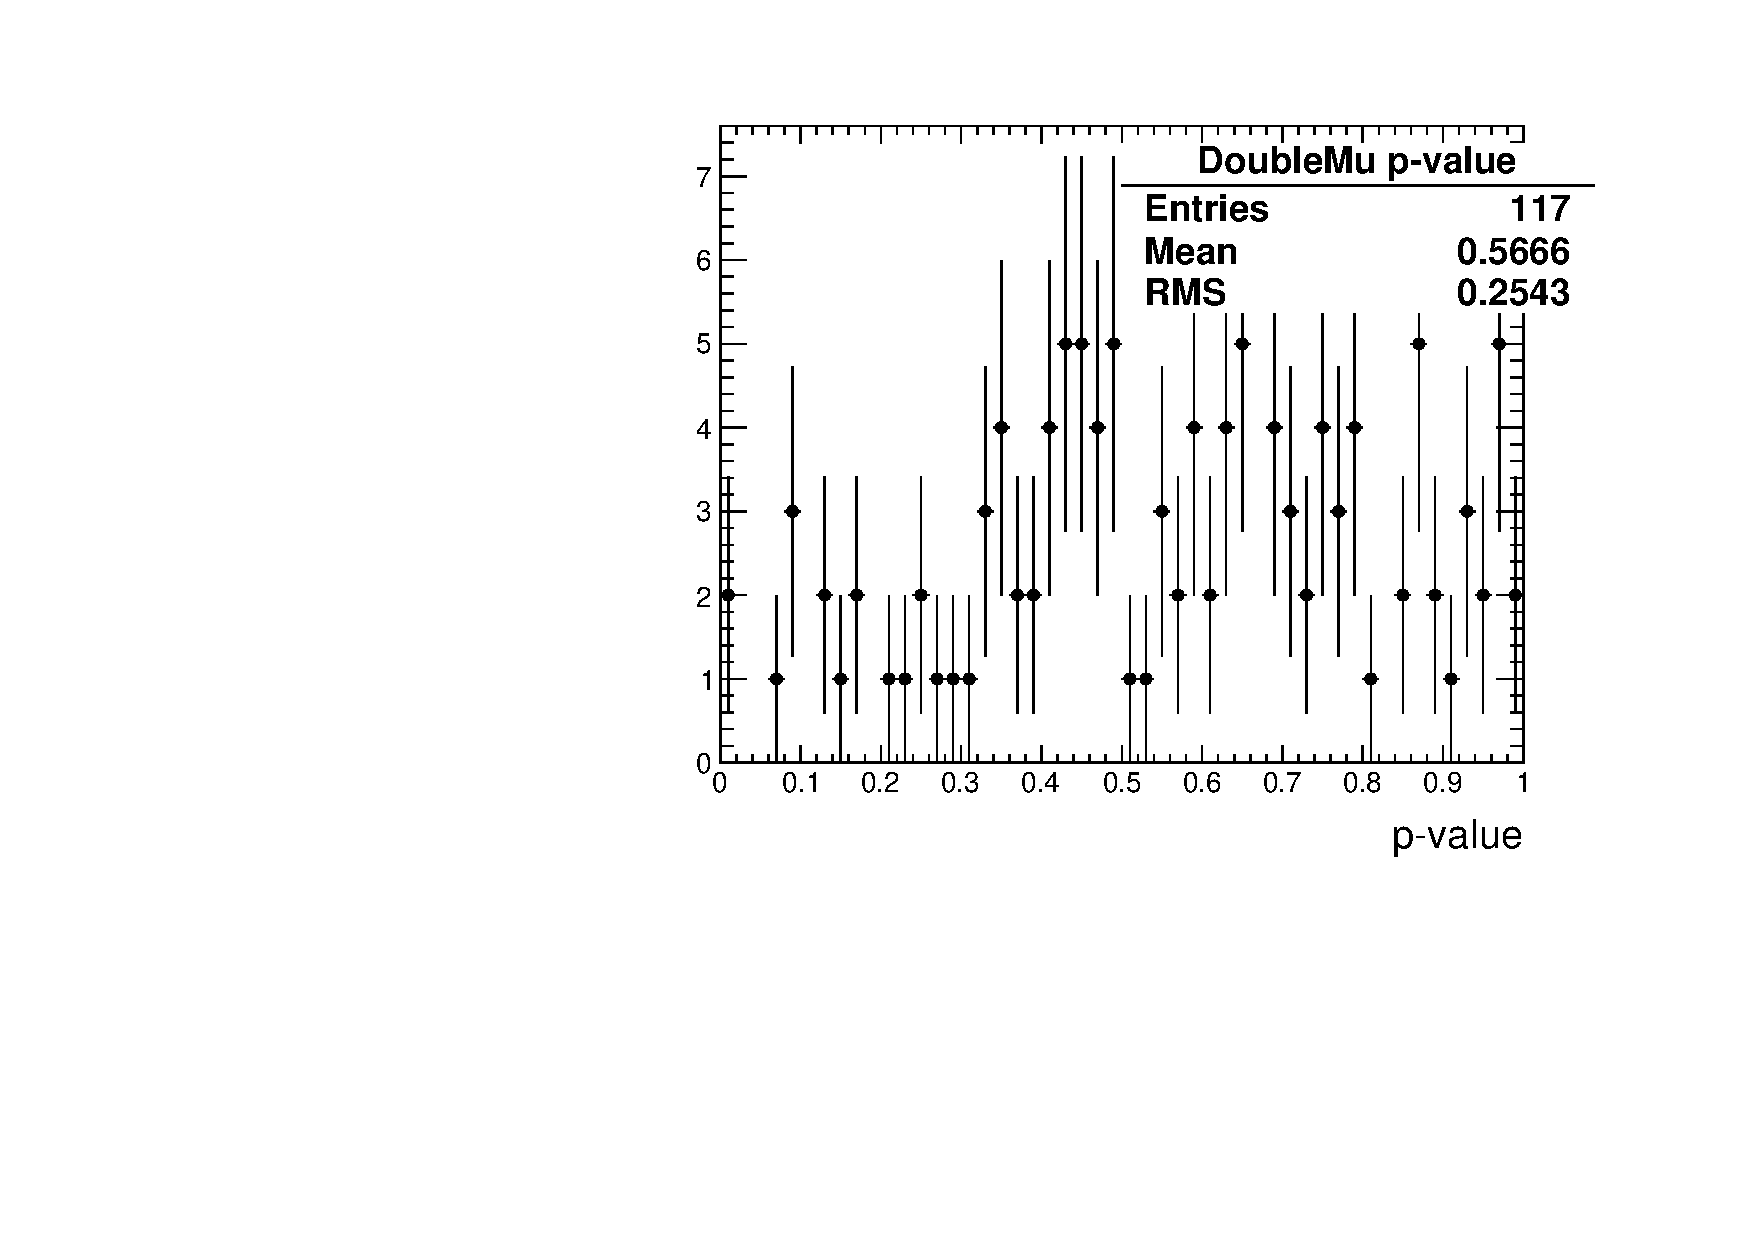
\includegraphics[width=0.45\textwidth]{Figures/backgroundPrediction/shapeOutput12Fb/scale_ht_variable_mht/DoubleMu/fitOut/Linear2DShiftMean/pValue_Linear2DShiftMean_DoubleMu.pdf}
  }~~
  \\
  \caption{\label{fig:pValues} The distributions of the p-value for the linear fit.} 
\end{figure}
\subsection{Deriving systematics on the \mht~shape}
\label{sec:systMhtDimension}

The systematic uncertainty in the \mht~shape is extracted from
the statistical precision to which the zero bias hypothesis can
be confirmed using the control regions, as described in the following.

Each background in the signal region (\ttbar/W  and \zInv~) is predicted 
using several control regions. In order to determine the uncertainty in
the \mht~shape, a combined linear fit is made over all relevant control regions. 
A requirement of at least 10 events and a non-trivial
number of degrees of freedom is made to ensure a reasonable fit. Where this
requirement is not satisfied, the \mht~distribution is not used in the signal region.
An \mht~requirement of 130 \GeV~is made to ensure a similar phase space to 
the signal region.
The uncertainty on the linear parameter from the fit is then
used to define the $\pm 1 \sigma$ variations of the nominal template.
As a conservative estimate, the systematic uncertainty in each category, and separately
for \zInv~and \ttbar/W, is defined using the best fit value of the $p_1$ parameter 
from the simultaneous fit to the relevant control regions
added in quadrature to its uncertainty.

An additional validation is carried out by comparing expected and observed uncertainties
on the linear parameter defining the template variations.
The expected uncertainties are derived by using a linear fit to the simulation/simulation ratio where the numerator
is treated as data. The relative uncertainties per 100 \GeV~from the weighted mean of \mht
for \ttbar/W and \zInv~ are shown in Figure~\ref{fig:expectedObservedTtw} 
and Figure~\ref{fig:expectedObservedZinv} and compared to those observed.
These show good agreement, which provides additional motivation for the 
zero bias hypothesis as well as validating the method for deriving expected uncertainties.


\begin{figure}[h!]
  \centering
  \subfloat[\label{fig:expectedTtw} Expected uncertainties]{
    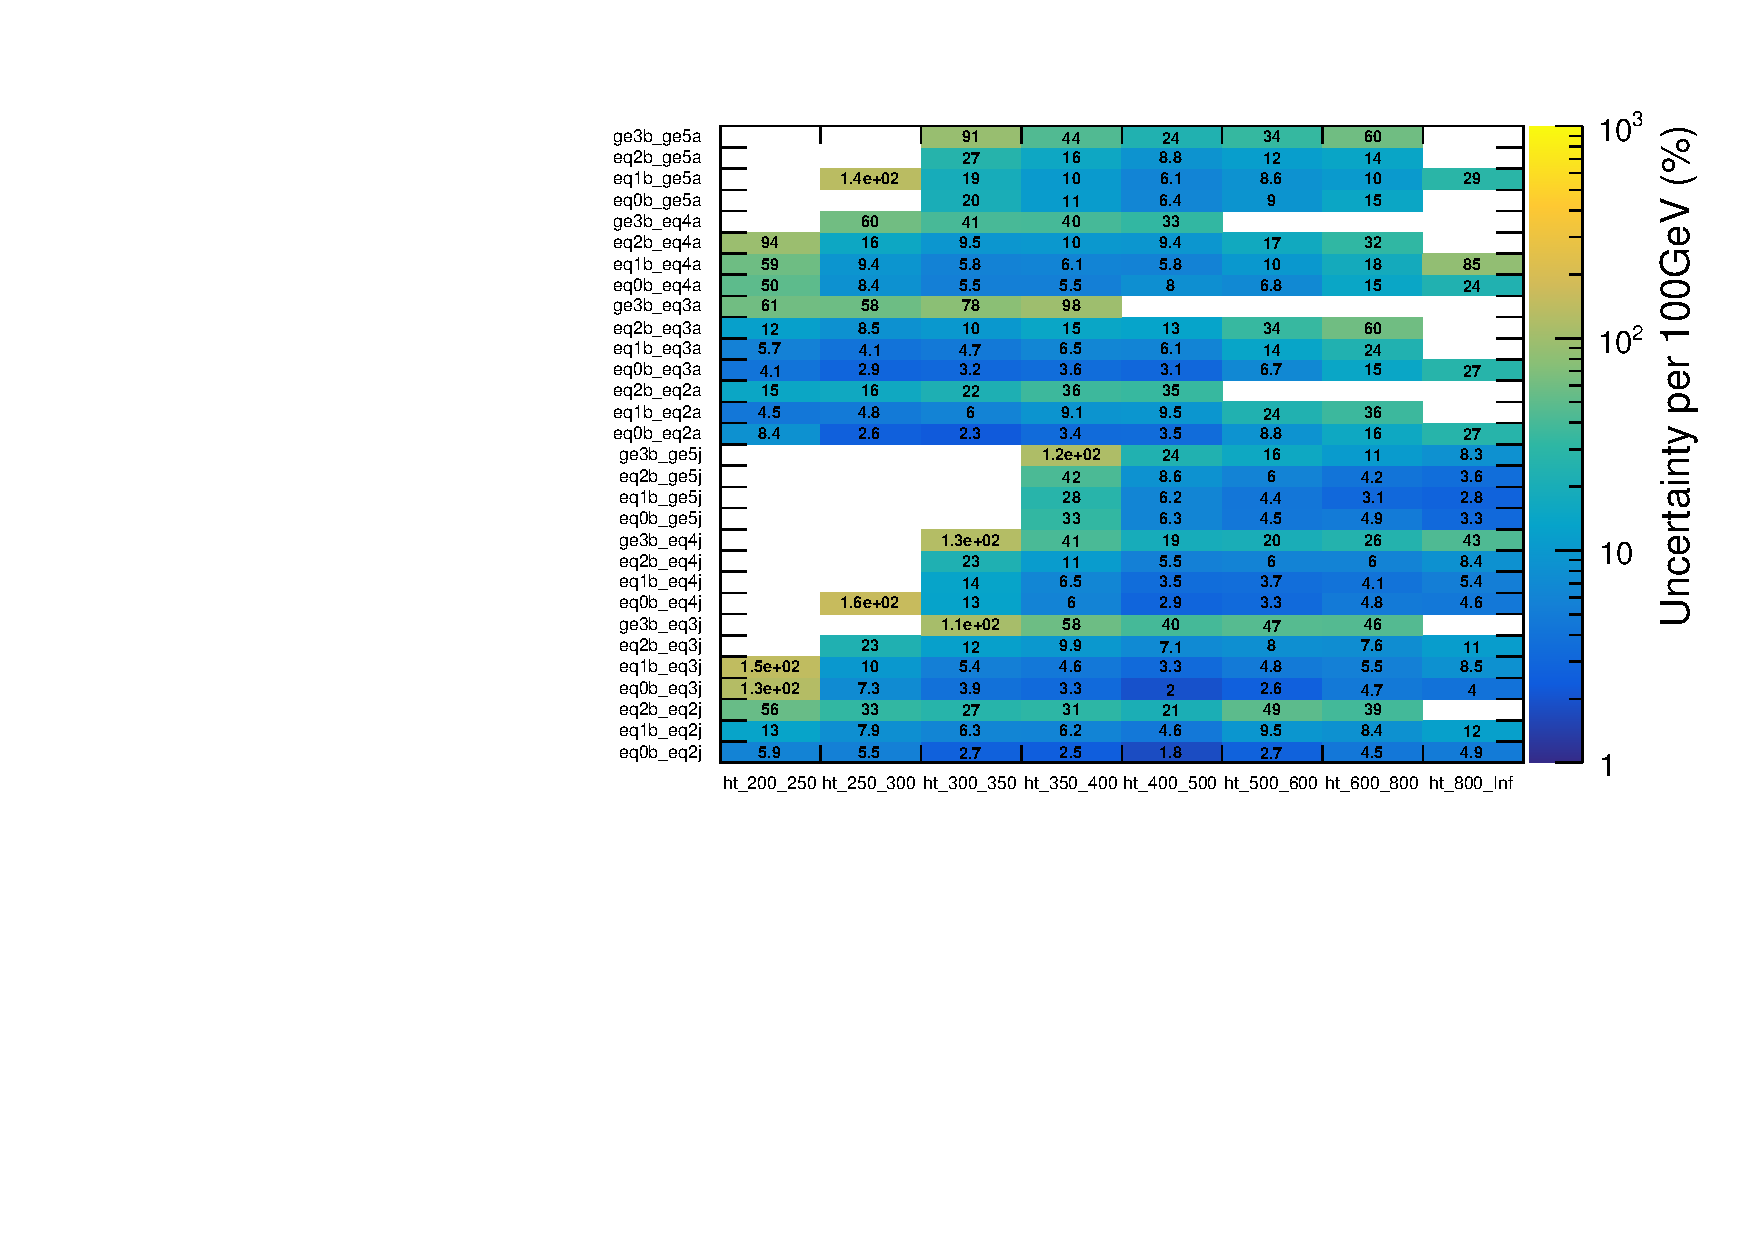
\includegraphics[width=0.45\textwidth]{Figures/backgroundPrediction/shapeOutput12FbMC/scale_ht_variable_mht/Ttw/fitOut/Linear2DShiftMean/frenchFlagErrComplete_Linear2DShiftMean_p1_Ttw.pdf}
  }~~
  \subfloat[\label{fig:observedTtw} Observed uncertainties]{
    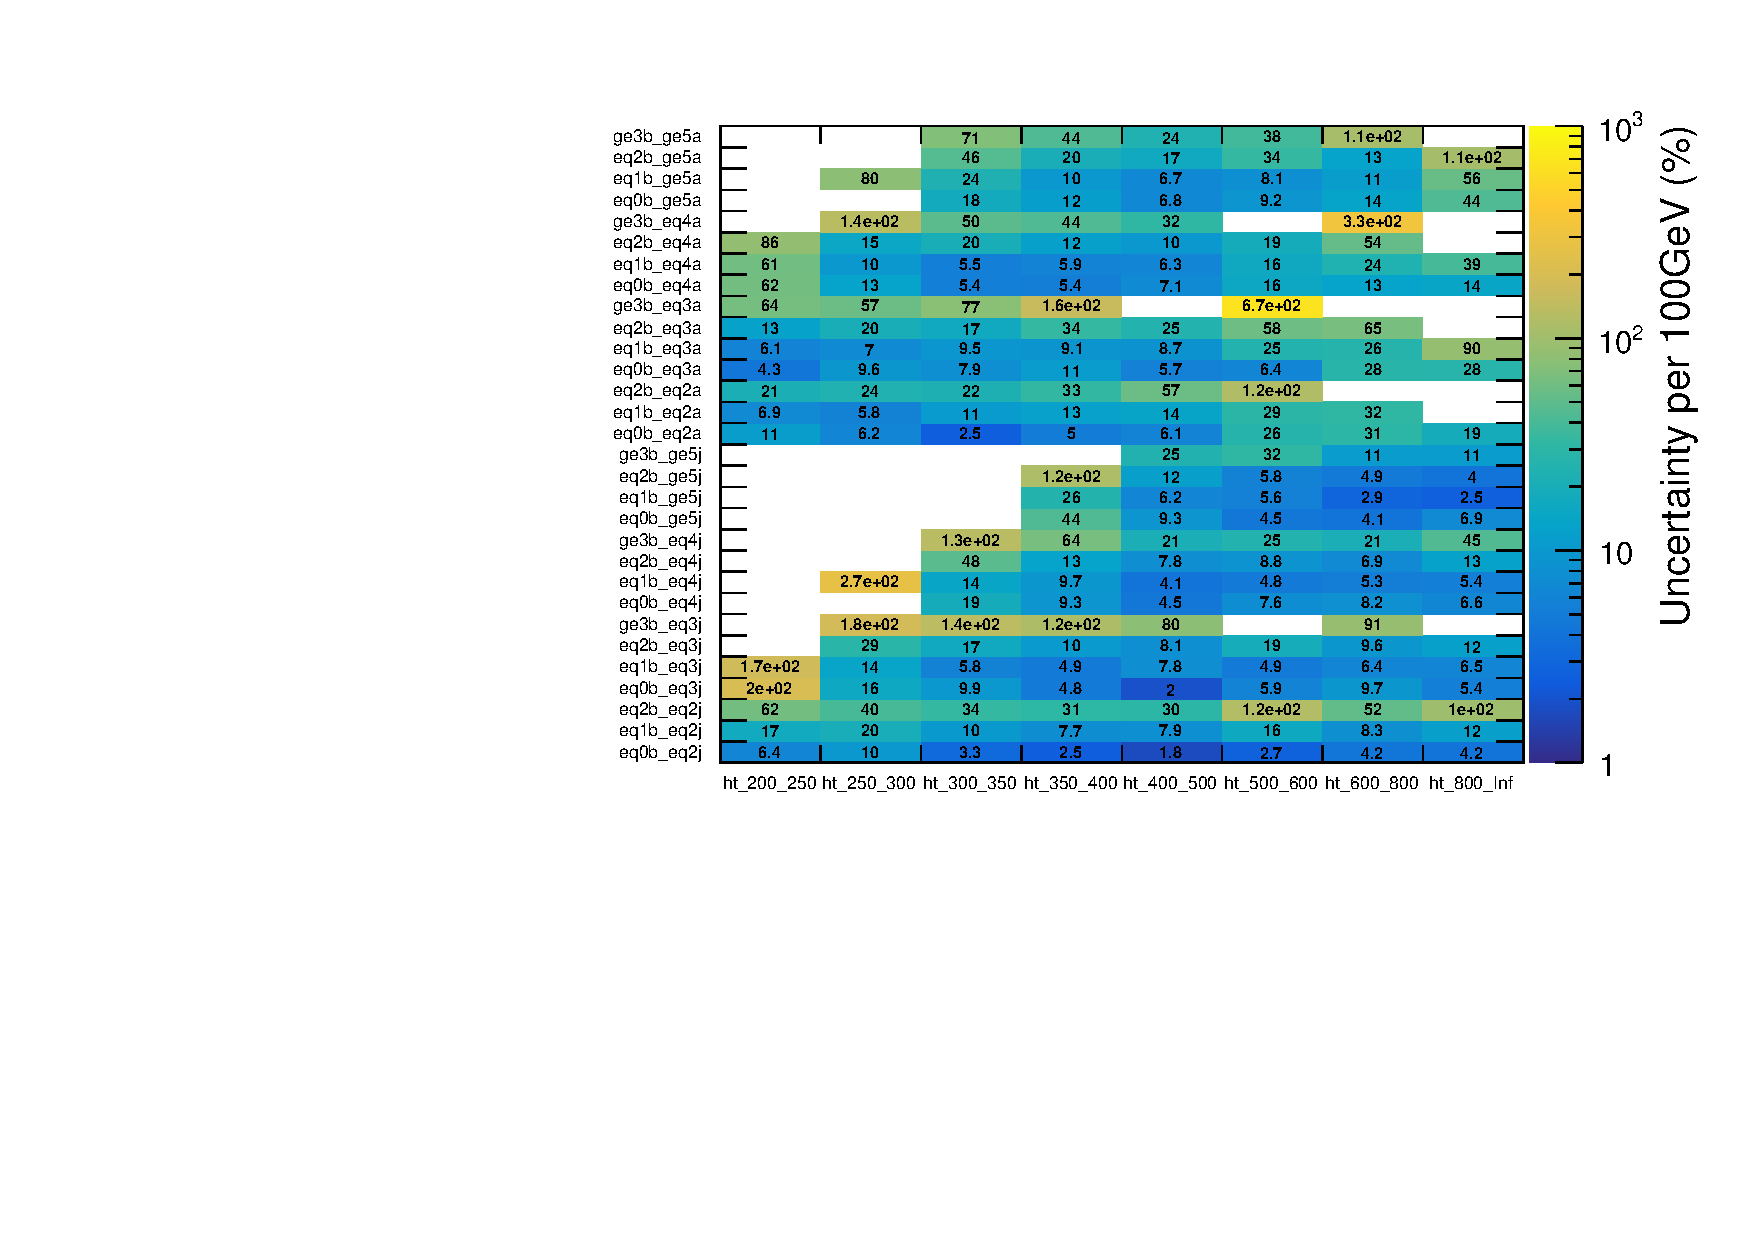
\includegraphics[width=0.45\textwidth]{Figures/backgroundPrediction/shapeOutput12Fb/scale_ht_variable_mht/Ttw/fitOut/Linear2DShiftMean/frenchFlagErrComplete_Linear2DShiftMean_p1_Ttw.pdf}
  }\\
  \caption{\label{fig:expectedObservedTtw} Expected relative uncertainties per 100 \GeV~shown for \ttbar/W in (a) are consistent
  with observed uncertainties shown in (b).}
\end{figure}

\begin{figure}[h!]
  \centering
  \subfloat[\label{fig:expectedZinv} Expected uncertainties]{
    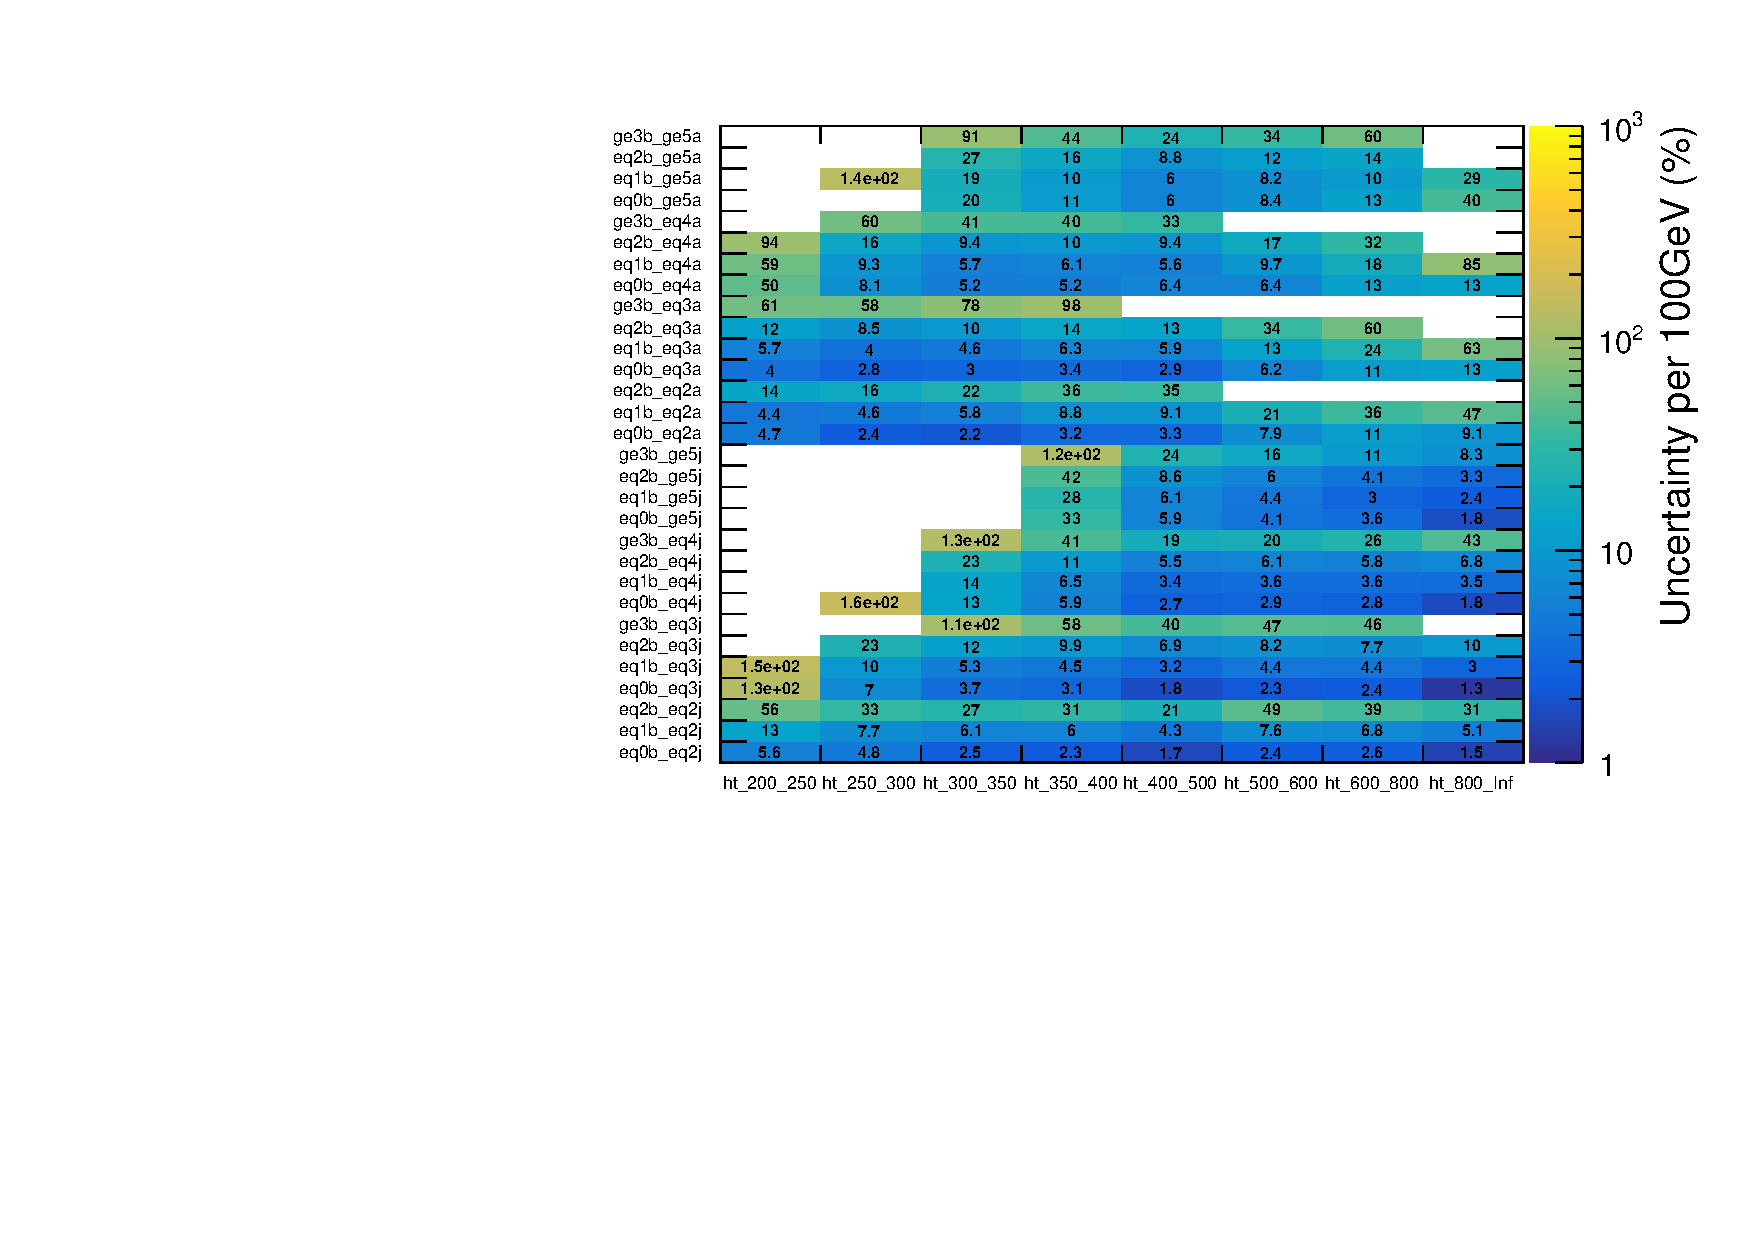
\includegraphics[width=0.45\textwidth]{Figures/backgroundPrediction/shapeOutput12FbMC/scale_ht_variable_mht/Zinv/fitOut/Linear2DShiftMean/frenchFlagErrComplete_Linear2DShiftMean_p1_Zinv.pdf}
  }~~
  \subfloat[\label{fig:observedZinv} Observed uncertainties]{
    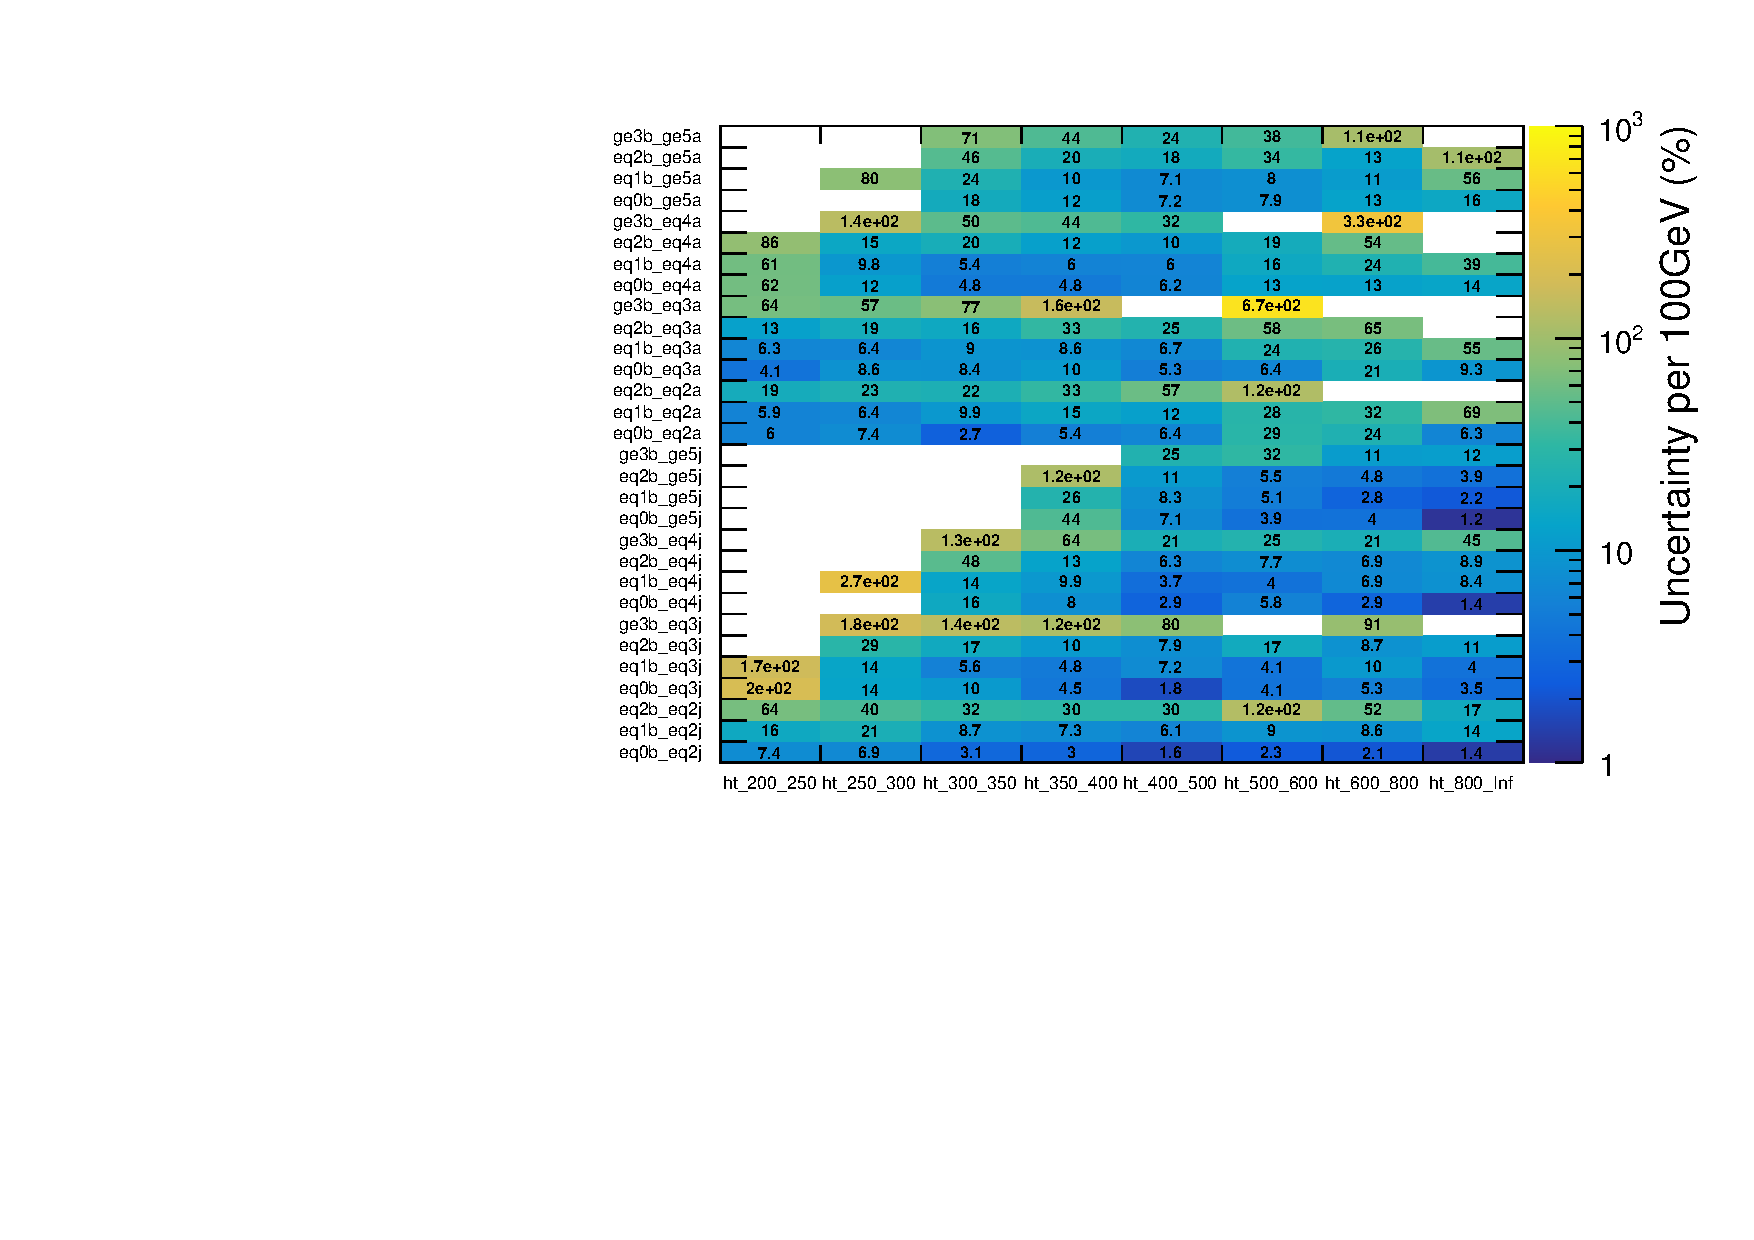
\includegraphics[width=0.45\textwidth]{Figures/backgroundPrediction/shapeOutput12Fb/scale_ht_variable_mht/Zinv/fitOut/Linear2DShiftMean/frenchFlagErrComplete_Linear2DShiftMean_p1_Zinv.pdf}
  }\\
  \caption{\label{fig:expectedObservedZinv}Expected relative uncertainties per 100 \GeV~shown for \zInv~ in (a) are consistent
  with observed uncertainties shown in (b).}
\end{figure}


\newpage
\subsection{Inclusion of systematic sources from simulation}
\label{sec:mcSystStudiesShape}

The effects on the \mht~shape of the uncertainties derived from variations in simulation 
(described in Section~\ref{sec:syst-uncs-var}) are included within the likelihood.
In this section, the size of the variation of the \mht~distribution under $\pm1\sigma$ shifts of the
sources of systematic uncertainty and the linear OP systematic uncertainty
described in \ref{sec:valid13} are compared. In the likelihood, the \mht~shape and transfer factors
are varied simultaneously for each source of uncertainty, as discussed in Section~\ref{sec:likelihood}.

To study the effect of the systematic variations on the \mht~shape, 
figure~\ref{fig:mcCompHighLow} shows the \mht~variations in two representative \scalht~bins 
and jet categories. The templates for each $\pm 1 \sigma$ variation are normalised to the
nominal template such that only the shape is varied.

% \begin{figure}[h!]
%   \centering
%   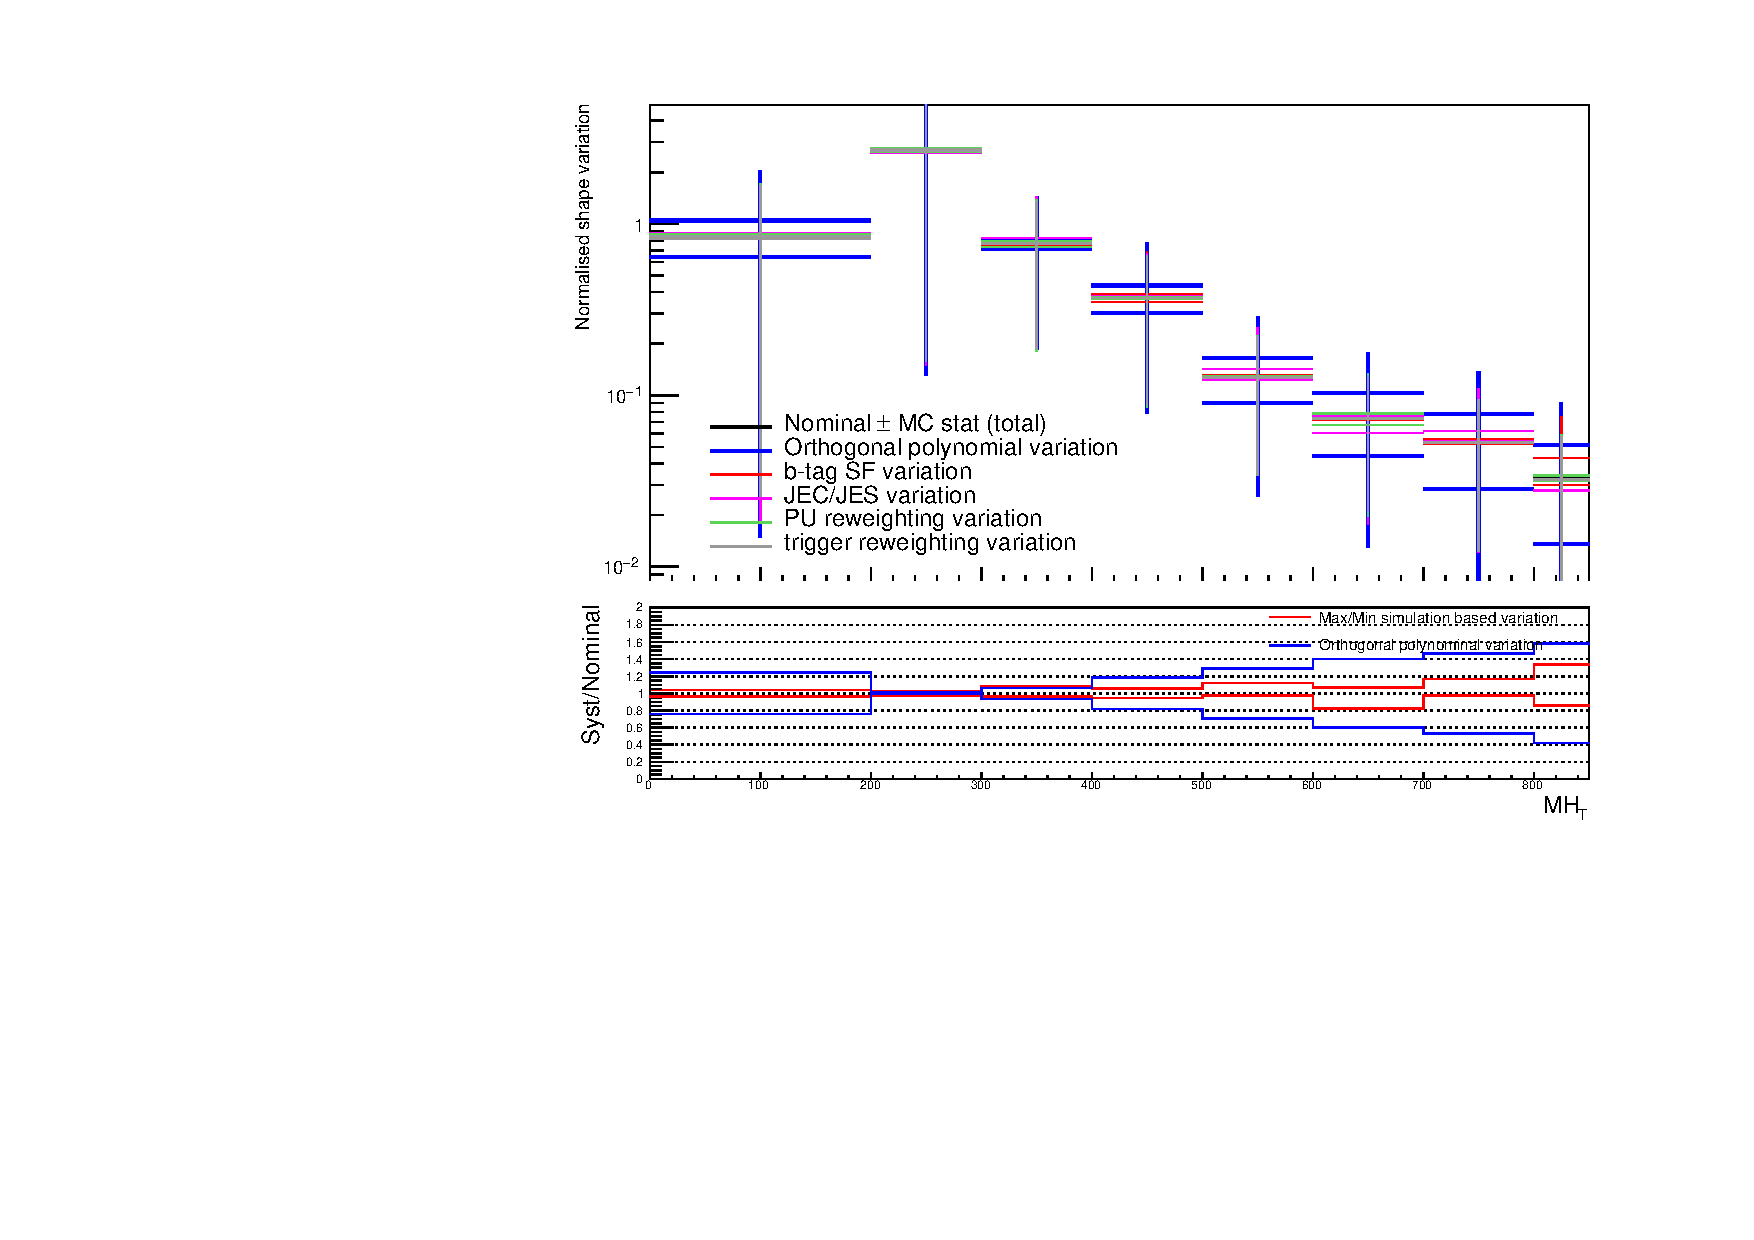
\includegraphics[width=0.6\textwidth]{Figures/backgroundPrediction/mcComparison6fb/totalSMS-T1tttt_mGluino-1000_mLSP-100_25ns_mht_ge5j_ge3b_800.pdf}
%   \caption{\label{fig:mcCompLow} Simulation derived systematic variations compared to the linear OP
%   data-driven systematic for an example bin \scalht $800-\infty$, \njet $\geq 5$, \nb $\geq 2$.}
% \end{figure}
% \begin{figure}[h!]
%   \centering
%   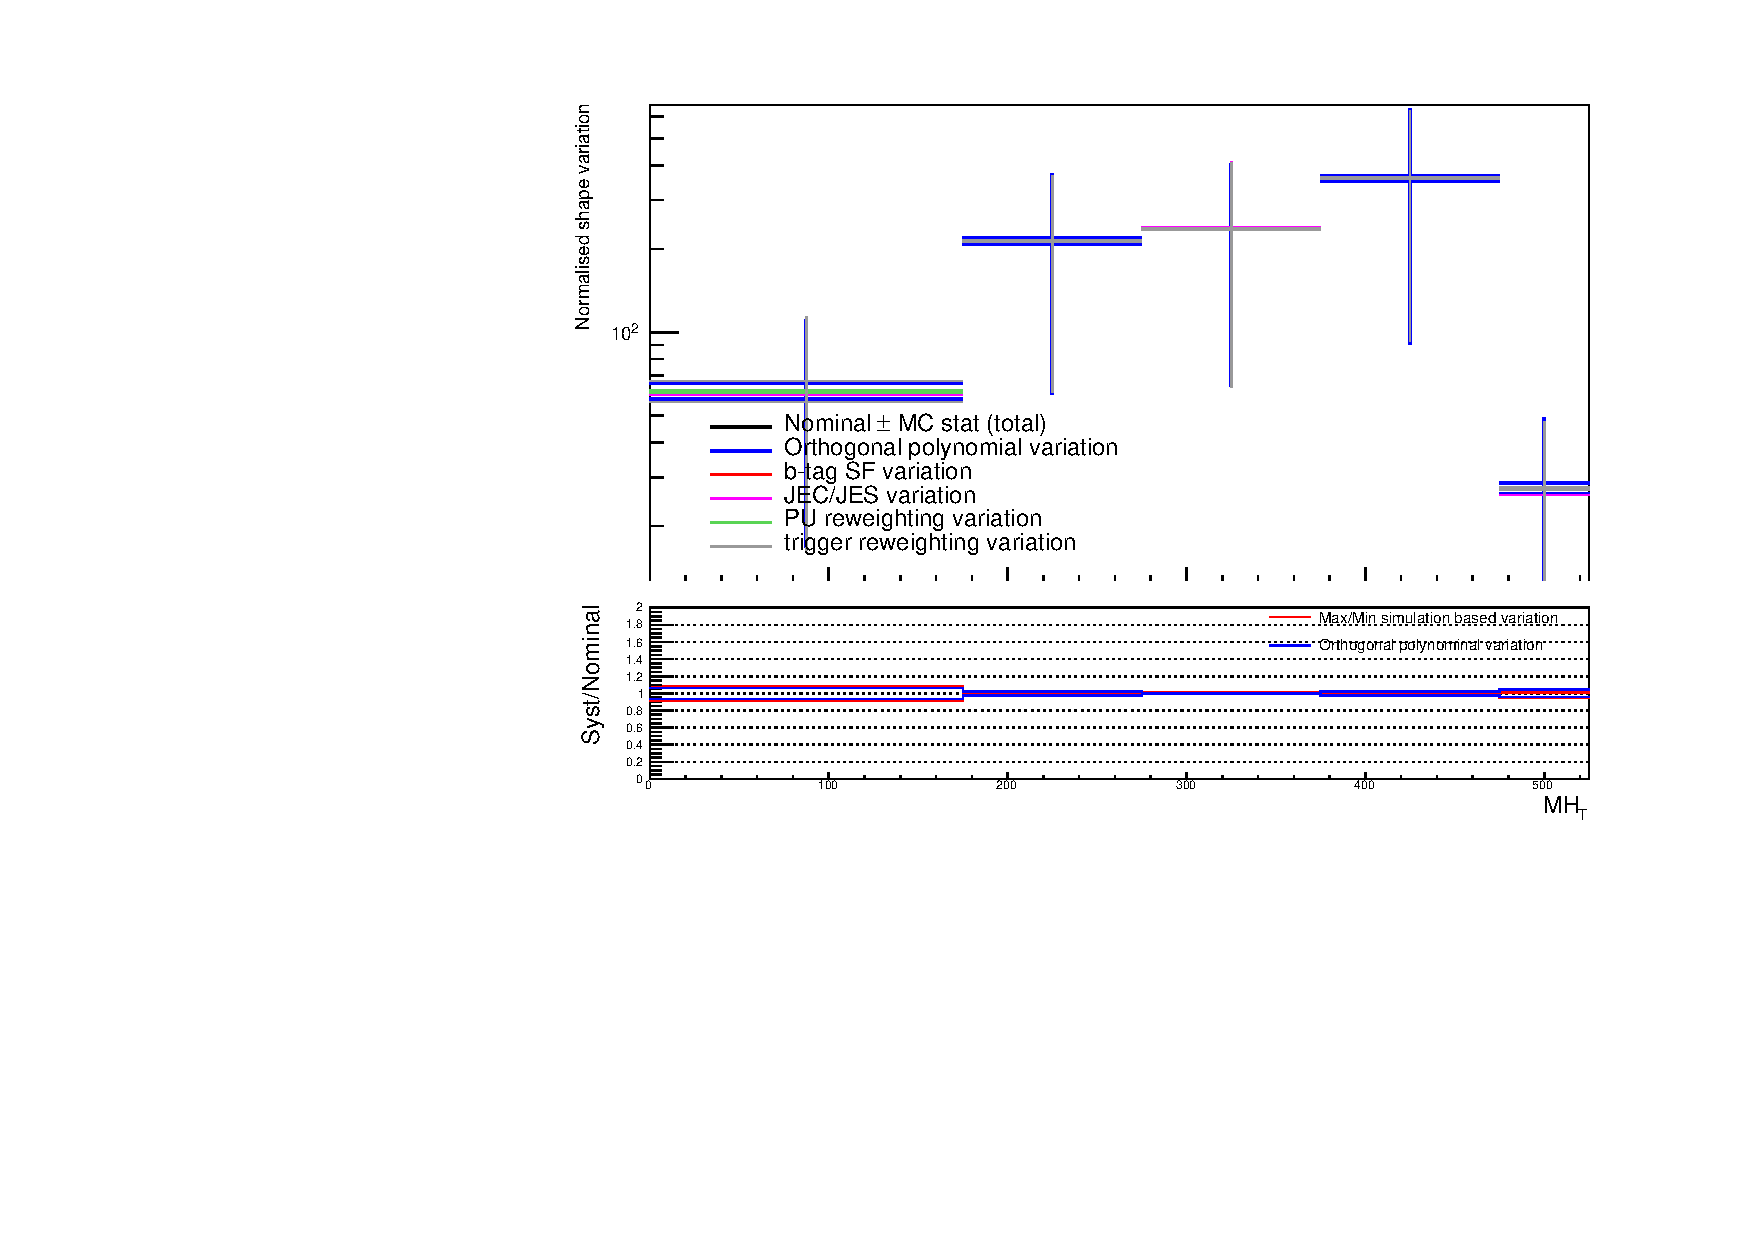
\includegraphics[width=0.6\textwidth]{Figures/backgroundPrediction/mcComparison6fb/totalSMS-T1tttt_mGluino-1000_mLSP-100_25ns_mht_eq2j_eq0b_400.pdf}
%   \caption{\label{fig:mcCompHigh} 
%   Simulation derived systematic variations compared to the 
% linear OP data-driven systematic for an example bin \scalht 400-500, \njet $= 2$, \nb $= 0$.}
% \end{figure}
\begin{figure}[h!]
  \centering
  \subfloat[\label{fig:mcCompLow} \scalht $800-\infty$, \njet $\geq 5$, \nb $\geq 2$]{
    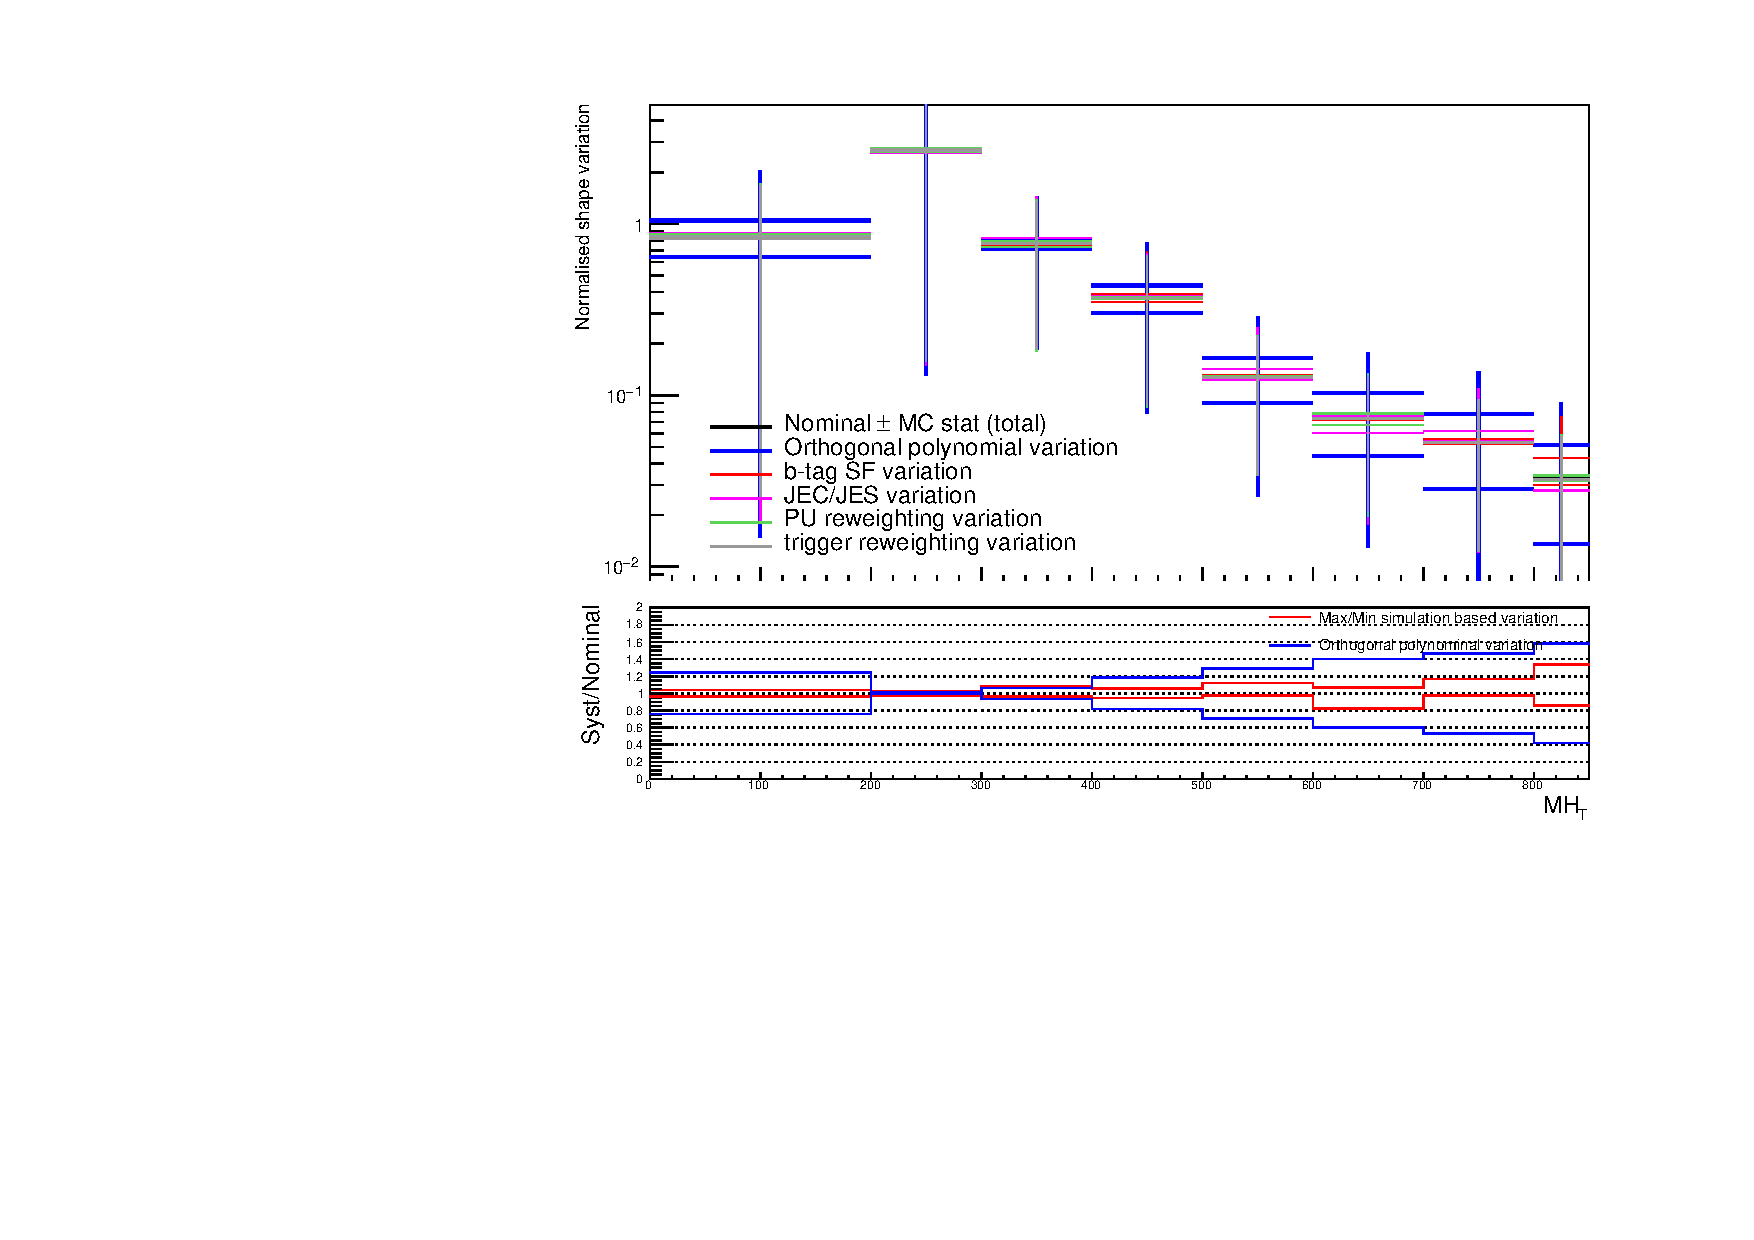
\includegraphics[width=0.45\textwidth]{Figures/backgroundPrediction/mcComparison6fb/totalSMS-T1tttt_mGluino-1000_mLSP-100_25ns_mht_ge5j_ge3b_800.pdf}
  }~~
  \subfloat[\label{fig:mcCompHigh}  \scalht 400-500, \njet $= 2$, \nb $= 0$]{
    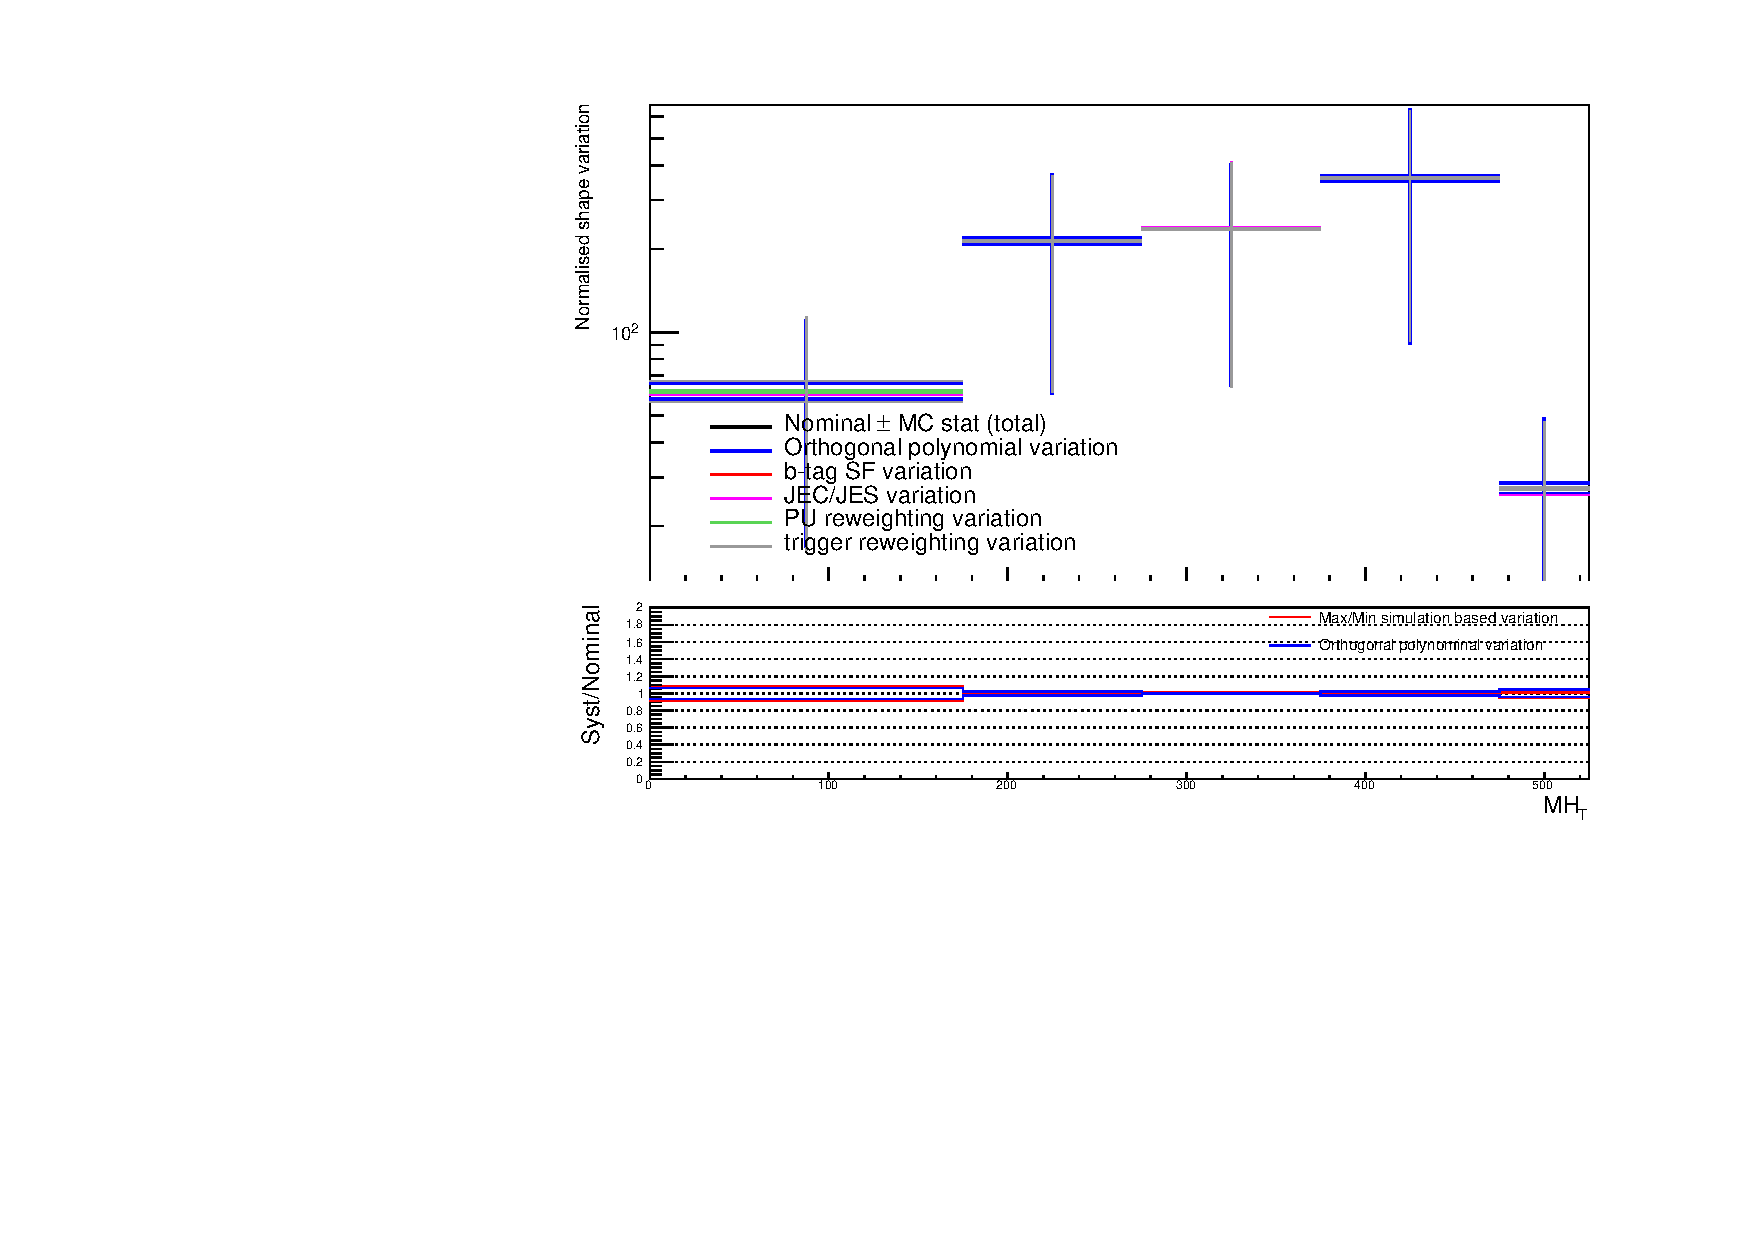
\includegraphics[width=0.45\textwidth]{Figures/backgroundPrediction/mcComparison6fb/totalSMS-T1tttt_mGluino-1000_mLSP-100_25ns_mht_eq2j_eq0b_400.pdf}
  }\\
  \caption{\label{fig:mcCompHighLow}
  Simulation derived systematic variations on the \mht distribution compared to the 
linear OP data-driven systematic for two representative categories.}
\end{figure}

\section{Summary}

The methods described in this section provide a robust estimation of the 
contributions from both electroweak and QCD multijet background sources
as well as the corresponding systematic uncertainties. These
predictions must be confronted with the observed data using the 
likelihood model described
in Chapter~\ref{cha:statisticalResults}.

% \begin{figure}[h!]
% \centering
% \subfloat[Upwards deviation]{
% \includegraphics[width=0.45\textwidth]{Figures/backgroundPrediction/mcComparison6fb/lastBinRatioMax.pdf}
% }
% \subfloat[Downwards deviation]{
% \includegraphics[width=0.45\textwidth]{Figures/backgroundPrediction/mcComparison6fb/lastBinRatioMin.pdf}
% }\\
% \caption{\label{fig:lastBinVar} Maximum upwards and downwards variations in the last \mht bin as a proportion of the orthogonal polynomial deviation}
% \end{figure}


